\documentclass[12pt,a4paper, twoside]{article}
\usepackage[utf8]{inputenc}
\usepackage{amsmath}
\usepackage{amsfonts}
\usepackage{amssymb}
\usepackage{graphicx}
\usepackage{enumitem}
\author{Marco Bertenghi}
\usepackage{amsthm}
\usepackage{xcolor}
\usepackage{mdframed}
\usepackage{centernot}
\date{}
\usepackage{subfiles}
\usepackage[centering, a4paper]{geometry}
\usepackage{fancyhdr}
\pagestyle{fancy}

\fancyhead[RE]{\rightmark}
\fancyhead[RO]{}
\fancyhead[LO]{\leftmark}
\fancyhead[LE]{}

\newtheorem{lem}{Lemma}[section]
\newtheorem{thm}{Theorem}[section]
\newtheorem{prop}{Proposition}[section]
\newtheorem{cor}{Corollary}[section]
\newtheorem{defn}{Definition}[section]
\newtheorem{exe}{Exercise}[section]
\newtheorem{exmp}{Example}[section]
\theoremstyle{definition}
\newtheorem{rem}{Remark}[section]


\usepackage{color}  
\usepackage{hyperref}
\hypersetup{
    colorlinks=false, %set true if you want colored links
    linktoc=all,     %set to all if you want both sections and subsections linked
    linkcolor=blue,  %choose some color if you want links to stand out
}

\newenvironment{rcases}
  {\left.\begin{aligned}}
  {\end{aligned}\right\rbrace}
  
\newcommand{\EE}{\mathbb{E}} %expectation
\newcommand{\PP}{\mathbb{P}} %probability
\newcommand{\teq}{\overset{\wedge}{=}}
\newcommand{\simple}{\textbf{\text{b}}\mathcal{E}}
\newcommand{\pred}{\textbf{\text{b}}\mathcal{P}}
\newcommand{\verysimple}{\textbf{\text{b}}\mathcal{E}_{\text{det}}}
\newcommand{\sign}{\text{sign}}
\newcommand{\MV}{\text{MV}}

\DeclareMathOperator*{\esssup}{ess\,sup}

\begin{document}
\begin{titlepage}
	\centering
	
	{\scshape\LARGE University of Zurich \par}

	\vspace{1cm}
	{\huge\bfseries Mathematical Finance\par}
		\vspace{2cm}
		\begin{mdframed}[backgroundcolor=blue!20, topline=true, linewidth=2.0pt]
\begin{flushleft}\textbf{Theorem} (Itô's formula): Let $(X_t)_{t \geq 0} = (X_t^1, \dots , X_t^d)_{t \geq 0}$ be an $\mathbb{R}^d$-valued semimartingale and let $F \in C^2 ( \mathbb{R}^d, \mathbb{R})$.  Denote $X_{s-}:= \lim_{u \nearrow s} X_u$, $\Delta X_s^j: = X_s^j-X_{s-}^j$ the associated jump-process and $[ X^j, X^k]^c$ denotes the quadratic variation of the continuous components of $X^j$ and $X^k$. \\ Then $(F(X_t))_{t \geq 0}$ is again a semimartingale and we have
\end{flushleft}
\begin{align*}
F(X_t)-F(X_0)= \sum_{j=1}^d \int_0^t \dfrac{\partial F}{\partial x_j} (X_{s-}) dX_s^j + \frac{1}{2} \sum_{j,k=1}^d \int_0^t \dfrac{\partial^2  F}{\partial x_j \partial x_k}(X_{s-}) d [ X^j, X^k ]_s^c \\
+ \sum_{0 < s \leq t} \left( F(X_s)-F(X_{s-}) - \sum_{j=1}^d \dfrac{\partial F}{\partial x_j} (X_{s-}) \Delta X_s^j \right). 
\end{align*}
\end{mdframed}
\par\vspace{1cm}
	\vspace{2cm}
	{\Large\itshape Transcribed by \par Marco Bertenghi\par}
	\vfill
	Based on the lecture notes of \par
	Prof. Martin \textsc{Schweizer} (ETHZ)

	\vfill

% Bottom of the page
	{\large \today\par}
\end{titlepage}
\newpage
\tableofcontents
\newpage
\section{Introduction and Preliminaries}
We start by recalling some important definitions and discuss the general setup we are working with in a heuristic manner. 
\begin{defn} Given a filtered probability space $(\Omega, \mathcal{F}, ( \mathcal{F}_n)_{n \in \mathbb{N}}, \mathbb{P})$ and a discrete-time stochastic process $(X_n)_{n \in \mathbb{N}}$. We say $(X_n)_{n \in \mathbb{N}}$ is predictable if $X_{n+1}$ is measurable with respect to the $\sigma$-algebra $\mathcal{F}_n$ for each $n \in \mathbb{N}$. 
\end{defn}

\begin{defn} Given a filtered probability space $(\Omega, \mathcal{F}, ( \mathcal{F}_n)_{n \in \mathbb{N}}, \mathbb{P})$, then a continuous-time stochastic process $(X_t)_{t \geq 0}$ is predictable if $X$, considered as a mapping from $\Omega \times \mathbb{R}_+$, is measurable with respect to the $\sigma$-algebra generated by all left-continuous adapted processes. This $\sigma$-algebra is also called the predictable $\sigma$-algebra. 
\end{defn}
\begin{exmp} The following are easy examples of predictable processes.
\begin{itemize}
\item Every deterministic process is a predictable process.
\item Every continuous-time adapted process that is left-continuous is predictable.
\end{itemize}
\end{exmp}
We will now start with basic ideas, not all will be defined in detail here, consult later sections of this script. 
\\\\
\textbf{Setup}: We are given a \textbf{time horizon} $T \in (0, \infty)$, \textbf{trading dates} $t \in [0,T],$ a filtered probability space $( \Omega, \mathcal{F}, ( \mathcal{F}_t)_{0 \leq t \leq T}, \mathbb{P})$ with the filtration satisfying the usual conditions (i.e. it is complete and right-continuous). Intuitively, $\mathcal{F}_t$ describes the information (events observable) up to time $t.$ 
\\\\
Typically we are given one reference asset with positive price, $\widetilde{S_t^0}>0$, for all $t$ which is adapted. Often called \textbf{bank account, bond, savings account} etc. Moreover, we are given $d$ \textbf{"risky" assets} with price process $\widetilde{S^i}=(\widetilde{S_t^i})_{0 \leq t \leq T}$, so $\widetilde{S}$ is a $\mathbb{R}^d$-valued stochastic process that is also adapted. Intuitively, $\widetilde{S_t^i}$ is the time-$t$ price (in some units) of one unit (share) of asset $i$.
\\\\
We agree on the following \textbf{simplifications}: express all prices in units of reference asset $\widetilde{S^0},$ so asset $0$ has (new) unit price of $1$ and $S^i:= \widetilde{S^i}/\widetilde{S^0}$ are prices (in units of asset $0$) of $d$ risky assets. Thus we usually start with model $(1,S)$ with $S$ being an adapted $\mathbb{R}^d$-valued stochastic process (almost always assume that $S$ is RCLL (\textbf{R}ight \textbf{C}ontinuous with \textbf{L}eft \textbf{L}imits) or in French càdlàg (\textbf{c}ontinue \textbf{à} \textbf{d}roite, \textbf{l}imite \textbf{à} \textbf{g}auche)), with $d+1$ assets where $d \geq 1$. 
\\\\
Common terminology for the above simplifications is to say that $S$ is \textbf{asset-0-discounted}.
\newpage
Here are two examples.

\begin{exmp}[Cox-Ross-Rubinstein/binomial model] This is a discrete-time model, described by $\widetilde{S_k^0 }=(1+r)^k$ and ($d=1$) $\widetilde{S_k^1}/\widetilde{S_{k-1}^1}$ i.i.d. with values $1+u,1+d$ with probability $p$ respectively $1-p$. In other words, a multiplicative random walk with drift. 
\end{exmp}

\begin{rem} We can naturally "transform" discrete into continuous-time models by taking the filtration $\mathbb{F}$ and processes to be piecewise constant. 
\end{rem}

\begin{exmp}[Black-Scholes model or Geometric Brownian Motion] Bank account with (continuous compounding) interest rate $r$, so $\widetilde{S_t^0}=e^{rt}$ and $(d=1)$ 
\begin{align*}
\widetilde{S_t^1} = \exp \left( \sigma W_t + \left( \mu - \frac{1}{2} \sigma^2 \right) t \right),
\end{align*}
where $W$ denotes a Brownian motion. Thus
\begin{align*}
S_t^1 = \frac{\widetilde{S_t^1}}{\widetilde{S_t^0}} = \exp \left( \sigma W_t + \left( \mu - r - \frac{1}{2} \sigma^2\right)t \right),
\end{align*}
which satisfies by Itô's formula the SDE 
\begin{align*}
d S_t^1 = S_t^1 (( \mu-r)dt + \sigma dW_t).
\end{align*}
More generally, we can discuss the Itô process model which has
\begin{align*}
dS_t^i = S_t^i \left( b_t^i dt + \sum_{j=1}^n \sigma_t^{ij} d W_t^j \right)_{i=1, \dots , d} 
\end{align*}
with $\mathbb{R}^n$-valued Brownian motion $W$ and predictable $b$ ($\mathbb{R}^d$-valued) and $\sigma$ ($\mathbb{R}^{d \times n}$-valued). 
\end{exmp}
\newpage
We will now introduce further terminology/concepts in the same heuristic manner as before. 
\\\\
A \textbf{trading strategy} (or \textbf{dynamic portfolio}) is a stochastic process $\varphi = (\varphi_t)_{0 \leq t \leq T}$, $\varphi=( \varphi^0 , \vartheta)$ with $\varphi^0$ being $\mathbb{R}$-valued and $\vartheta$ being $\mathbb{R}^d$-valued. We interpret this as follows: at time $t$, we hold $\varphi_t^0$ units of asset $0$ and $\vartheta_t^i$ units of asset $i$ where $i=1, \dots , d$. 
\\\\
A \textbf{value process} $V(\varphi)= ( V_t( \varphi))_{0 \leq t \leq T}$, in units of reference asset $0$ is given by 
\begin{align*}
V_t( \varphi) = \varphi_t^0 1 + \sum_{i=1}^d \vartheta_t^i S_t^i = \varphi_t^{\text{tr}} (1S_t)
\end{align*}
which is the time-$t$ value of time-$t$ portfolio. 
\begin{rem} \
\begin{enumerate}
\item For easy of notation, often think of $d=1$, (i.e. one risky asset), this is usually harmless. 
\item In original (tilde) units, value is given by 
\begin{align*}
\widetilde{V_t}( \varphi)= \varphi_t^{\text{tr}} \widetilde{S_t} = \varphi_t^0 \widetilde{S_t^0} + \sum_{i=1}^d \vartheta_t^i \widetilde{S_t^i}, \text{ where }  \widetilde{S_t^i}= S_t^i \widetilde{S_t^0}.
\end{align*}
So clearly,  $\widetilde{V}(\varphi)= \widetilde{S_0}V( \varphi)$. 
\end{enumerate}
\end{rem}
\noindent \textbf{The costs of the strategy}: if we keep $\varphi$ constant between $t$ and $t + \Delta t$ and only change it from $\varphi_t$ to $\varphi_{t + \Delta t}$ at $t + \Delta t$ this gives on $(t,t+ \Delta t]$ expenses or \textbf{cost-increment} 
\begin{align*}
C_{t + \Delta t} - C_t &= ( \varphi_{t + \Delta t } - \varphi_t)^{\text{tr}} (1 S_{t + \Delta t}) \\
&= \varphi_{t + \Delta t}^0 - \varphi_t^0 + ( \vartheta_{t + \Delta t} - \vartheta_t)^{\text{tr}} S_{t + \Delta t }  \\
&= \underbrace{\varphi_{t + \Delta t}^0 + \vartheta_{t + \Delta t}^{\text{tr}} S_{t + \Delta t}}_{= V_{t + \Delta t}} \underbrace{- \varphi_t^0 - \vartheta_t^{\text{tr}} S_t}_{= - V_t( \varphi)}- \varphi_t^{\text{tr}} S_{t+ \Delta t} + \vartheta_t^{\text{tr}} S_t  \\ 
&= V_{t + \Delta t} ( \varphi) - V_t( \varphi) - \vartheta^{\text{tr}}( S_{t + \Delta t} - S_t). 
\end{align*}
Adding up and letting $\Delta t \to 0$ suggests that the natural definition of total cost on $[0,t]$ of strategy $\varphi$ is given by 
\begin{align*}
C_t( \varphi) = V_t( \varphi)- \int_0^t \vartheta_u d S_u, \ 0 \leq t \leq T. 
\end{align*}
(Note: integrand $\vartheta$ is naturally evaluated at left end $t$ of interval $(t, t + \Delta t]$.)
\newpage
\begin{rem} In original units, costs on $[0,t]$ is 
\begin{align*}
\widetilde{V_t}( \varphi) = \widetilde{V_t}( \varphi) - \int_0^t  \vartheta_u d \widetilde{S_u},
\end{align*}
note that then $\widetilde{C}( \varphi) \neq S^0 C( \varphi)$. 
\end{rem}
In \textbf{discrete time}, $S$ is piecewise constant and the previous integral $\int \vartheta d S$ reduces to a sum. Only condition needed for $\vartheta$ , on economic grounds, is that stock holdings $\vartheta_{k+1}$ on $[k,k+1)$ must be determined at beginning $k$ of interval $[k,k+1)$, so $\vartheta_{k+1}$ must be $\mathcal{F}_k$-measurable for all $k$,  i.e. $\vartheta$ must be predictable (needed to exclude insiders or prophets). No extra conditions on $\varphi^0$, it can be adapted. 
\\\\
In \textbf{continuous time}, by analogy,  still impose that $\vartheta$ is predictable and $\varphi^0$ is adapted. But to have $\int \vartheta d S$ well-defined, need that $S$ is a \textbf{semimartingale} and $\vartheta$ is $S$-integrable, we will discuss this in more detail later; if $S$ happens to be a continuous semimartingale, then we know from Brownian Motion and Stochastic Calculus lectures what a sufficient condition for $S$-integrability is. 
\begin{rem} $V( \varphi), C( \varphi), \int \vartheta dS$ are always real valued (clear from the interpretation). If $\vartheta$ and $S$ are $\mathbb{R}^d$-valued, then $\int \vartheta dS$ denotes the vector stochastic integral 
\begin{align*}
" \int \sum \vartheta^i dS^i ";
\end{align*}
this may be different from 
\begin{align*}
\sum \int \vartheta^i d S^i. 
\end{align*}
The latter may fail to be well-defined. Here $d>1$ needs technical care. 
\end{rem}
\begin{defn} A strategy $\varphi = ( \varphi^0, \vartheta)$ is called \textbf{self-financing} if $C( \varphi)\equiv C_0( \varphi)$, i.e. $C_t( \varphi) = C_0( \varphi)$ $\mathbb{P}$-almost surely for all $t$. 
\end{defn}
We interpret the above definition as follows: after initial outlay of $C_0( \varphi)= V_0( \varphi)$ trading according to $\varphi$ generates neither expenses nor surplus. 
\newpage
\begin{lem} \label{L01} \
\begin{enumerate}
\item A strategy $\varphi=( \varphi^0, \vartheta)$ is self-financing if and only if  $V( \varphi) = V_0( \varphi) + \int \vartheta dS$. 
\item (Reparametrisation): There exists a bijection between self-financing strategies $\varphi = ( \varphi^0, \vartheta)$ and pairs $(v_0, \vartheta) \in L^0( \mathcal{F}_0) \times \{\text{predictable, $S$-integrable processes}\}$. Explicitly, $v_0= V_0( \varphi)$ and conversely $\varphi_0= v_0 + \int \vartheta dS - \vartheta^{\text{tr}}S$.
\item If $\varphi= ( \varphi^0, \vartheta)$ is self-financing, then $\varphi^0$ is predictable. 
\end{enumerate}
\end{lem}
\begin{rem} Part 2) of the above lemma is extremely useful: Can specify self-financing strategies by giving initial wealth/capital $v_0$ and prescribing arbitrary trading pattern (predictable, $S$-integrable) in the $d$ risky assets. Self-financing requirement then automatically determines what one must do in asset $0$. This is very often used in literature without explicit mention. Crucially needs existence of reference asset $\widetilde{S^0} >0$. 
\end{rem}
\begin{proof} \
\begin{enumerate}
\item 
\begin{align*}
V( \varphi)\overset{\text{def}}=C( \varphi) + \int \vartheta dS \overset{\text{self-fin.}}= C_0( \varphi) + \int \vartheta dS = V_0( \varphi) + \int \vartheta dS. 
\end{align*}
\item Mapping $(v_0, \vartheta) \mapsto ( \varphi^0, \vartheta)$ is injective and resulting $\varphi$ is self-financing, this is easy to check using 1) as 
\begin{align*}
V( \varphi) = \varphi^0 1 + \vartheta^{\text{tr}}S = v_0 + \int \vartheta dS = V_0( \varphi) + \int \vartheta dS. 
\end{align*}
Easy to check that mapping is surjective, using $v_0=V_0( \varphi)$ to recover a given $\varphi^0$. 
\item Needs one result from stochastic calculus. For any RCLL process $Y=(Y_t)_{0 \leq t \leq T}$ denote by $\Delta Y_t := Y_t -Y_{t^-} = Y_t - \lim_{s \to t, s <t} Y_s$ the jump of $Y$ at $t$. From stochastic integration theory, we need 
\begin{align*}
\Delta \left( \int \vartheta dS\right)_t = \vartheta_t^{\text{tr}} \Delta S_t = \vartheta_t^{\text{tr}}(S_t-S_{t^-}).
\end{align*}
So we get from 2) that 
\begin{align*}
\varphi_t^0 &= v_0 + \int_0^t \vartheta dS - \vartheta_t^{\text{tr}} S_t 
= v_0 + \int_0^{t^-} \vartheta_u dS_u + \Delta \left( \int \vartheta dS\right)_t - \vartheta_t^{\text{tr}} S_t \\
&= v_0 + \int_0^{t^-} \vartheta_u dS_u - \vartheta_t^{\text{tr}} S_{t^-}
\end{align*}
We have $v_0$ is $\mathcal{F}_0$-measurable and thus predictable, $\int_0^{t^-} \vartheta_u dS_u$ is LC, adapted and thus predictable, $\vartheta_t^{\text{tr}}$ is predictable by assumption, $S_{t^-}$ is LC and adopted, hence predictable, which concludes that $\varphi_t^0$ is predictable. 
\end{enumerate}
\end{proof}
The previous lemma establishes that in the model $(1,S)$, we can identify self-financing $\varphi$ with $(v_0, \vartheta) \in L^0( \mathcal{F}_0) \times \{$predictable, $S$-integrable processes$\}$, via $V( \varphi)= v_0 + \int \vartheta d S$. We use the notation
\begin{align*}
\varphi \teq (v_0, \vartheta).
\end{align*}
\begin{rem}[Important] Take $v_0=0$ and look at $\varphi \teq (0, \vartheta)$. Then 
\begin{align*}
G(\vartheta):= \int \vartheta dS = 0 + \int \vartheta dS = V((0, \vartheta))=V(\varphi)
\end{align*}
is value process of a self-financing strategy starting with zero initial wealth and trading according to $\vartheta$. In particular 
\begin{align*}
G_T( \vartheta) = \int_0^T \vartheta_u dS_u
\end{align*}
is final wealth one can generate via self-financing trading using $\vartheta$ from $0$ initial capital. This will come up very often. 
\end{rem}
\begin{rem} \ \begin{itemize}
\item Note that $\varphi \teq (0, \vartheta)$ and $\vartheta$ are different objects and will be distinguished - $\varphi$ is self-financing strategy, whereas $\vartheta$ is integrand for $S$. 
\item Also note that the identification needs the existence of $S^0 \equiv 1$. 
\end{itemize}
\end{rem}
\newpage
During our treatise so far we have made many \textbf{implicit assumptions}. Let us list them here for clarification:
\begin{itemize}
\item Can trade \textbf{continuously in time}.
\item All agents have \textbf{same information}.
\item Prices for buying and selling are both given by $S$: no \textbf{transaction costs}/\textbf{frictionless trading}.
\item The integrand $\vartheta$ is $\mathbb{R}^d$-valued, $\varphi^0$ is $\mathbb{R}$-valued, so $\vartheta_t^i, \varphi_t^0$ can take arbitrary values in $\mathbb{R}$, no \textbf{trading constraints} (like e.g. minimal lot size, integer number of units, short sales of stocks ($\vartheta_t^i < 0)$ and borrowing reference asset $( \varphi_t^0 < 0)$ allowed. 
\item Asset prices are exogenously given by fixed model $(1,S)$, do not react to trading strategies: \textbf{small investors/price takers}. In consequence, "book value" $V( \varphi)$ is also market/liquidation value.
\item Probability measure $\PP$ and hence law of $S$ are known, \textbf{no uncertainty about underlying probability model} (of course, the price evaluation $t \mapsto S_t( \omega)$ is still unknown, because $\omega \in \Omega$ is unknown). 
\end{itemize}
Self-financing strategies are a reasonable requirement. But one cannot allow \textbf{all} self-financing $\varphi$; some restrictions are needed as the next example demonstrates. 
\begin{exmp} Take $d=1$, and $S=W$ a standard Brownian motion. For ease of exposition, work on infinite time horizon $[0, \infty)$.
\begin{exe} Construct similar example on $[0,T]$ and with $S>0$. 
\end{exe}
Define $\tau:= \inf \{ t \geq 0 : W_t=1 \}$. This $\tau$ is a stopping time and (LIL: Law of Iterated Logarithm) $\tau < \infty$ $\PP$-a.s. Define 
\begin{align*}
\vartheta:= 1_{(\!(0, \tau]\!]}
\end{align*}
(notation $(\!(0, \tau ]\!] := \{ ( \omega, t) \in \Omega \times [0, \infty) : 0 < t \leq \tau (\omega) \})$. We notice that $\vartheta$ is adapted and left-continuous, hence predictable, moreover it is bounded. So $\vartheta$ is $S$-integrable, and $\varphi \teq (0, \vartheta)$ has wealth given by 
\begin{align*}
V(\varphi)= \int \vartheta dS = W^\tau - W_0 = W^\tau=W_{t \wedge \tau}
\end{align*}
and in particular final value given by 
\begin{align*}
V_\infty( \varphi)= W_\infty^\tau = W_{\tau \wedge \infty} = W_\tau \equiv 1.
\end{align*}
Thus $\varphi$ starts from $0$, is self-financing and ends up with wealth $1$, which is clearly a \textbf{money pump}!
\end{exmp}
\newpage
Let us discuss the \textbf{problem} that has become evident in the previous example: The value process $V( \varphi) = W^\tau$ is unbounded from below.
\begin{itemize}
\item Interpretation: must be able to \textbf{borrow unlimited} amounts!
\end{itemize}
Consequently we should probably impose lower bound on wealth for "good" self-financial strategies. 
\begin{itemize}
\item Why is $W^\tau$ unbounded from below?
\end{itemize}
Suppose for contradiction that $W^\tau \geq -a$ for some constant $a$. Then $W^\tau$ is a martingale (because BM $W$ is a martingale), hence a supermartingale and uniformly bounded from below by $a$. But then $W^\tau$ is closable on $[0, \infty]$ as super-martingale and so we can apply stopping theorem on $[0, \infty]$ to obtain 
\begin{align*}
1=\EE(W_\tau)=\EE( W_\infty^\tau) \leq \EE( W_0^\tau) = \EE(W_0)=0
\end{align*}
which gives a contradiction, hence $W^\tau = W_{t \wedge \tau}$ is indeed unbounded from below. 
\\\\
We conclude this introduction section by giving an overview of the \textbf{main topics} of this course:
\begin{enumerate}
\item \textbf{Arbitrage theory}: give precise mathematical description of idea that money pumps should be impossible, and characterize those models which satisfy this. Other models are not reasonable from economic/financial perspective.
\item \textbf{Pricing and hedging}: Start with reasonable model $(1,S)$. Fix $H \in L^0( \mathcal{F}_T)$ and view this as a random payoff to make at $T$ (due to financial contract. Can we find a self-financing $\varphi \teq = (v_0 \vartheta)$ with $V_T( \varphi)=H$ (or perhaps $ \geq H$, or close to $H$)? If yes, what is (perhaps minimal) required initial wealth $v_0$?
\item \textbf{Optimal investment}: Suppose again that $(1,S)$ is reasonable. Given initial wealth $v_0$, what is best investment strategy, i.e. which self-financing $\varphi \teq (v_0, \vartheta)$ produces "best" final wealth $V_T( \varphi) = v_0 +  \int_0^T \vartheta_u dS_u$? This is a control problem over variable $\vartheta$, and it requires (subject) criterion for comparing final wealths. 
\end{enumerate}
\newpage
\section{First ideas in arbitrage theory}
\textbf{Basic idea}: in a reasonable model of a financial market, money pumps should not exist. What is the mathematical formulation for this idea? How do we characterize such models?\\
\\
\textbf{Setup}: Given a filtered probability space $( \Omega, \mathcal{F}, \mathbb{F}, \PP)$ over $[0,T]$ with $S^0 \equiv 1$ and $S$ being $\mathbb{R}^d$-valued RCLL. 
\\\\
By Lemma \ref{L01} any $\mathbb{R}^d$-valued, predictable $\vartheta$ with $\int \vartheta dS$ well defined (which may need extra condition on $S$ and $\vartheta)$ induces self-financing $\varphi \teq (0, \vartheta)$ with wealth 
\begin{align*}
V_t( \varphi) = \int_0^t \vartheta_u dS_u = G_t( \vartheta), \ 0 \leq t \leq T.
\end{align*}
\begin{defn} Call strategy $\varphi$ \textbf{$a$-admissible} with $a \geq 0$ if $V( \varphi) \geq -a$, meaning $V_t( \varphi) \geq - a$ $\PP$-a.s. for all $t$ (if we can choose RCLL version for $V(\varphi)$ this is equivalent to $\mathbb{P}( V_t( \varphi) \geq - a, \forall t)=1)$. Call strategy $\varphi$ \textbf{admissible} if $a$-admissible for some $a \geq 0$. 
\end{defn}
\begin{itemize}
\item \textbf{Interpretation}: trader using $\varphi$ (admissible as above) has some bound on his wealth/debts. 
\end{itemize}
\begin{rem} \
\begin{itemize}
\item For $\varphi \teq (0, \vartheta)$, strategy $\varphi$ is $a$-admissible iff integrand $\vartheta$ is $a$-admissible, meaning that $\int \vartheta dS \geq -a$. Then write 
\begin{align*}
\vartheta \in \Theta_{\text{admin}}^a \text{ and } \Theta_{\text{adm}} = \bigcup_{a \geq 0 } \Theta_{\text{adm}}^a.
\end{align*}
\item For $\varphi \teq (v_0, \vartheta)$ only clear connection between admissibility for $\varphi$ and admissibility of $\vartheta$ is if $v_0$ is constant. In general, $v_0 \in L^0( \mathcal{F}_0)$ and so one cannot say much, unless $\mathcal{F}_0$ is trivial. 
\end{itemize} 
\end{rem}
\begin{defn} We say $\vartheta$ is a \textbf{simple integrand}, denoted by $\vartheta \in \simple$ if it is of the form 
\begin{align*}
\vartheta = \sum_{i=1}^n h_i 1_{(\!( \tau_{i-1}, \tau_i ]\!]}, \ n \in \mathbb{N}
\end{align*}
with stopping times $0 \leq \tau_0 \leq \tau_1 \leq \tau_n \leq T$ and $H_i \in L^\infty ( \mathcal{F}_{\tau_{i-1}}, \mathbb{R}^d)$, i.e. $h$ is $\mathbb{R}^d$-valued, $ \mathcal{F}_{\tau_{i-1}}$-measurable and bounded. If all $\tau_i$ (but not $h_i)$ are deterministic $t_i$, call $\vartheta$ \textbf{very simple} and write $\vartheta \in \verysimple$. 
\end{defn}
\newpage
\begin{rem} \
\begin{itemize}
\item If we take any $\vartheta \in \simple$, then for any $\mathbb{R}^d$-valued process $S$, the integral $ \int \vartheta dS$ is well-defined as 
\begin{align*}
G_\cdot ( \vartheta) = \int_0^\cdot \vartheta dS = \sum_{i=1}^n h_i^{\text{tr}}(S^{\tau_i}- S^{\tau_{i-1}}) 
\end{align*}
so that 
\begin{align*}
G_T( \vartheta) = \sum_{i=1}^n h_i^{\text{tr}} (S_{\tau_i}-S_{\tau_{i-1}}).
\end{align*}
If $S$ is adapted RCLL, then so is $G( \vartheta)$. 
\item For model with finite discrete time $k=0,1, \dots , T \in \mathbb{N}$, we have
\begin{align*}
\simple = \{\text{all bounded $\mathbb{R}^d$-valued predictable processes}\}.
\end{align*}
\end{itemize}
\end{rem}
Let us now come back to our discussion of arbitrage opportunities:
\begin{itemize}
\item For \textbf{general $S$, simple arbitrage opportunity} is $\vartheta \in \simple$, admissible, with $G_T( \vartheta) \in L_+^0\setminus \{0 \}$ i.e. $G_T( \vartheta) \geq 0$ $\PP$-a.s. with $\PP( G_T( \vartheta) >0)>0$, start from initial capital $v_0=0$, manage to keep debts bounded, trade via $\varphi \teq (0, \vartheta)$ in self-financing way, end up with final wealth $V_T( \varphi) = G_T( \vartheta) \geq 0$ and even positive $(>0)$ with positive probability. 
\item For \textbf{semimartingale $S$, (general) arbitrage opportunity} is integrand $\vartheta$ for $S$ ($\mathbb{R}^d$-valued, predictable, $S$-integrable, so that $\int \vartheta dS$ is well-defined) which is admissible, with $G_T( \vartheta) \in L_+^0 \setminus \{0\}$. 
\end{itemize}
\newpage
We now give mathematical sound definitions for the absence of arbitrage conditions. Let us introduce the notation $G_T( \Theta):= \{ G_T( \vartheta) : \vartheta \in \Theta\}$.
\begin{mdframed}[backgroundcolor=yellow!20, topline=true, linewidth=2.0pt] \textbf{Absense of arbitrage conditions:}\\
\\
For general $S$ we impose the following conditions:
\begin{itemize}
\item (NA$_{\text{elem}})$: $G_T(\simple) \cap L_+^0 = \{ 0 \}$. 
\item (NA$_{\text{elem}}^\text{adm}$): $G_T(\simple \cap \Theta_\text{adm}) \cap L_+^0 = \{0\}$. 
\item (NA$_\text{det}$): \ $G_T(\verysimple) \cap L_+^0 = \{0\}$.
\end{itemize}
For semimartingale $S$ we only impose:
\begin{itemize}
\item (NA) $G_T( \Theta_\text{adm}) \cap L_+^0 = \{0 \}$. 
\end{itemize}
\end{mdframed}
\begin{rem} Notice that a better notation for (NA) would be (NA$^\text{adm})$ because we insist on the integrand $\vartheta$ being admissible (i.e. $a$-admissible for some $a \geq 0$). But in literature this is never done, hence we do so here as well. 
\end{rem}
Giving a sufficient condition is easy, as described by the Lemma below: 
\begin{lem} \label{L21} Suppose $S$ is adapted $\mathbb{R}^d$-valued. If there exists a probability measure $Q \approx \PP$ such that $S$ is a local $Q$-martingale, then both (NA$_\text{elem}^\text{adm})$ and (NA) hold. However, (NA$_\text{det}$) (and hence also (NA$_\text{elem}$) can fail. 
\end{lem}
\begin{proof} \
\begin{exe} Counterexample for (NA$_\text{det}$). 
\end{exe}
\noindent Notice that (NA$_\text{elem}^\text{adm})$ follows from (NA), because $\simple \cap \Theta_\text{adm} \subset \Theta_\text{adm}$. \\
\\
We first show that $S$ is actually a semimartingale under the assumption of the Lemma. Indeed, $S$ is by assumption a $Q$-local martingale, and $Q \approx \PP$, so the claim follows from general \textbf{Girsanov Theorem}. Thus we can talk about (NA) (which is only defined for semimartingales).
\\\\
From stochastic calculus, if $S$ is a semimartingale and $\vartheta$ is predictable, $S$-integrable, then $G( \vartheta)= \int \vartheta dS$ is well-defined and again a semimartingale. But if $S$ is actually a local martingale,  then $\int \vartheta dS$ must \textbf{not} be a local martingale (counterexample by Emery, uses $S$ with jumps)
\newpage
However, if $S$ is a local martingale, $\vartheta$ is predictable, $S$-integrable and if $G( \vartheta)= \int \vartheta dS$ is uniformly bounded from below (i.e. if $\vartheta \in \Theta_\text{adm})$, then $\int \vartheta dS$ is again a local martingale (Ansel/Stricker). Then, of course, by Fatou $\int \vartheta dS$ is also a supermartingale. 
\\\\
We now argue (NA): $S \in \mathcal{M}_\text{loc}(Q)$ and $\vartheta \in \Theta_\text{adm}$ (this is same under $Q$ since $\PP \approx Q)$,  thus $\int \vartheta dS \geq -a$ almost surely by admissibility. By our excursion above this shows that $\int \vartheta dS$ is a $Q$-supermartingale. So
\begin{align*}
\EE_Q(G_T( \vartheta)) \leq \EE_Q(G_0( \vartheta))=0.
\end{align*}
If now also $G_T( \vartheta) \geq 0$ $\PP$-a.s., then also $Q$-a.s. (since $Q \approx \PP)$, so we must have $G_T( \vartheta)=0$ $Q$-a.s. hence $\PP$-a.s. and so (NA) holds. 
\end{proof}
\begin{rem} Above supermartingale argument will come up again several times. 
\end{rem}
\begin{defn} An equivalent (local) martingale measure for $S$ is a probability measure $Q \approx \PP$ such that $S$ is a $Q$-(local) martingale. $Q$ is then called an E(L)MM. (Sometimes only ask for $Q \approx \PP$ on $\mathcal{F}_T)$. 
\end{defn}
With this definition in mind, we can rephrase Lemma \ref{L21}:
\begin{lem}[Rephrasing of Lemma \ref{L21}] Suppose there exists an ELMM for $S$, then $S$ satisfies (NA). 
\end{lem}
A natural question is then to ask if this sufficient condition is also necessary?
\begin{itemize}
\item \textbf{Answer}: For \textbf{finite discrete time} yes, see later. In general, the answer however is \textbf{no}! To get necessary and sufficient condition need something stronger than (NA). 
\end{itemize}
We will now illustrate problems by giving two examples:
\subsection{A counterexample in infinite discrete time}
Take $(Y_n)_{n \in \mathbb{N}}$ under $\PP$-independent with values $\pm 1$ and $\PP(Y_n= \pm 1)= 1/2(1+ \alpha_n)$. Define $S_0=1, \Delta S_n= S_n-S_{n-1}= \beta_n Y_n$. So $S$ is a binary random walk with drift. Take $\mathbb{F}= \mathbb{F}^Y= \mathbb{F}^S$ and $\mathcal{F}= \mathcal{F}_\infty$ if needed. \\
\\
Since $\Delta S_n$ only takes values $\pm \beta_n$, the only way to get $S$ a $Q$-martingale is to set $Q(Y_{n+1}= +1 \mid \mathcal{F}_n)= 1/2$ for all $n \in \mathbb{N}$. So the sequence $(Y_n)_{n \in \mathbb{N}}$ must be i.i.d. under $Q$ with $Q(Y_n=+1)=1/2$. This is the only candidate for an EMM. 
\begin{thm}[Kakutani's dichotomy theorem] In the above setting, $Q \approx \PP$ if and only if $\sum_{n=1}^\infty \alpha_n^2 < \infty$, otherwise, $Q \perp \PP$. 
\end{thm}
(Note: $Q \overset{\text{loc}}\approx \PP$ in the sense that $Q \approx \PP$ on $\mathcal{F}_n$ for all $n \in \mathbb{N}$, thus we need an infinite horizon to create problems.)
\newpage
Thus if we choose $(\alpha_n)_{n \in \mathbb{N}}$ such that $\sum_{n=1}^\infty \alpha_n^2 = + \infty$, then there is EMM for $S$. The role of $\beta_n$ so far is not important, if we choose $\sum_{n=1}^\infty \beta_n < \infty$, then $S$ is bounded, and then $S \in \mathcal{M}_{\text{loc}}$ is the same as $S \in \mathcal{M}$. Hence EMM is the same as ELMM, and so there can also \textbf{exist no} ELMM for $S$. \\
\\
\textbf{Claim}: Although $S$ does not admit any ELMM, it still satisfies (NA$_\text{elem}$). 
\begin{itemize}
\item Why not look at (NA)? Infinite horizon means that we should look at $G_\infty ( \vartheta)$, this is complicated for it is an infinite sum! For $\vartheta \in \simple$, $G( \vartheta)$ is a finite sum and $G_\infty( \vartheta)$ is no problem. 
\end{itemize}
Before we prove the claim, we need:
\begin{exe} There exists an arbitrage opportunity in $\simple$ if and only if there exists an arbitrage opportunity with $\vartheta$ of the form $\vartheta = h 1_{(\!(\sigma, \tau ]\!]}$ with $\sigma \leq \tau$ stopping times and $h \in L^\infty ( \mathcal{F}_0)$ (no admissibility here). 
\end{exe}
Now choose $\beta_n = 3^{-n}$ so that for every $m$ we have $\sum_{k=m+1}^\infty \beta_k < \beta_m$. This ensures that for $n >m$ the both conditions below hold:
\begin{align*}
\begin{cases} \sign(S_n-S_m)&= \sign(Y_{m+1}) \\
\sign(g(S_n-S_m))&= \sign(gY_{m+1}), \text{ for any RV } g. 
\end{cases}
\end{align*}
(Write $S_n-S_m = \sum_{k=m+1}^\infty \beta_k Y_k$, since the terms of the sequence of the sum are decreasing, only the first term is responsible for the sign)\\
\\
Take $\vartheta = h 1_{(\!( \sigma, \tau ]\!]}$ and compute: 
\begin{align*}
G_\infty ( \vartheta) = \int_0^\infty \vartheta_u d S_u = h ( S_\tau-S_\sigma).  
\end{align*}
It is \textbf{our goal} to show that if $G_\infty( \vartheta) \geq 0$ $\PP$-a.s., then in fact $G_\infty( \vartheta)=0 \ \PP$-a.s., this then implies that we have (NA$_\text{elem}$). \\
\\
Define for any $m \in \mathbb{N}$ the set $A_m:= \{ \sigma = m, \tau > m \} \in \mathcal{F}_m$. We then have: 
\begin{align*}
\sign(G_\infty( \vartheta))= \sign(H(S_\tau-S_\sigma)) = \sign(hY_{m+1}) \text{ on } A_m. 
\end{align*}
So if $G_\infty ( \vartheta) \geq 0 \ \PP$-a.s., we have $1_{A_m} \sign(hY_{m+1}) \geq 0$ for all $m \in \mathbb{N}$. We \textbf{claim} that this implies $h=0$ $\PP$-a.s. and then of course $G_\infty ( \vartheta)=0 \ \PP$-a.s. \\
\\
Indeed, $h$ is $\mathcal{F}_0$-measurable and $\sigma=m$ on $A_m$ (it can be shown that) this implies $h1_{A_m}$ is $\mathcal{F}_m$-measurable. Now, $0 \leq 1_{A_m} \sign(h1_{A_m}Y_{m+1})$ and because $h1_{A_m}$ is $\mathcal{F}_m$-measurable and $A_m \in \mathcal{F}_m, \ h 1_{A_m} Y_{m+1}$ must have the same sign on both $A_m \cap \{Y_{m+1}=+1\}$ and $A_m \cap \{Y_{m+1}=-1\}.$ But product $h1_{A_m} Y_{m+1}$ has on $A_m$ a unique sign ($ \geq 0$) and so we must have $h1_{A_m}=0$ $\PP$-a.s., this holds for all $m$ so that $h=0$ $\PP$-a.s. $\hfill \Box$
\newpage
\subsection{A counterexample in continuous time}
Start with a Brownian motion $W=(W_t)_{0 \leq t \leq T}$ and take as $\mathbb{G}$ natural (augmented) filtration of $W$. For $k(t):= 1/\sqrt{T-t}$, define 
\begin{align*}
Z_t := \begin{cases} \mathcal{E} \left( - \int_0^t k dW \right), & \text{ on } [0,T) \\ Z_T:= 0, & \text{ for } t=T
\end{cases}
\end{align*}
so that 
\begin{align*}
Z_t = \exp \left( - \int_0^t k(s) dW_s - \frac{1}{2} \int_0^t k^2 (s) ds \right),  \ 0 \leq t < T.
\end{align*}
With $\tau := \inf \{ t \in [0,T] : Z_t \geq 2 \} \wedge T$, $Z^\tau$ is a bounded martingale starting at $1$, and 
\begin{align*}
\begin{cases} Z_ \tau = 2, & \text{ if } \tau < T \\
Z_\tau = Z_T=0, & \text{ if } \tau = T
\end{cases}
\end{align*}
so that by the stopping theorem we get $\EE(Z_\tau) = \EE(Z_0)=1$ which readily implies $\mathbb{P}( \tau < T)=1/2$, because $\EE(Z_\tau)= E(2\cdot 1_{\tau < T} + 0 \cdot 1_{ \tau = T})=1$. Now define $S=(S_t)_{0 \leq t \leq T}$ as 
\begin{align*}
S_t = \begin{cases} W_t + \int_0^t k(s) ds, & \text{ for } t \leq \tau \\ S_\tau, & \text{ for } t \geq \tau \end{cases}
\end{align*}
and take (augmented) filtration $\mathcal{F}_t:= \mathcal{G}_{t \wedge T}$, $0 \leq t \leq T$, so that (up to nullsets) $\mathbb{F}= \mathbb{F}^S = \mathbb{F}^{W^\tau}$. \\
\\
Now Brownian motion has a martingale representation in its own filtration. Using this for $W^\tau$, we can conclude that all $( \mathbb{F}, \PP)$-local martingales must be stochastic integrals of $W^\tau$. By \textbf{Girsanov's theorem}, the only $Q \ll \PP$ which makes $S= S^\tau$ into a local $Q$-martingale must remove drift $k$ and hence must have density process $Z^\tau$ and $ \frac{dQ}{d\PP}= Z_\tau$. \\
\\
But $Z_\tau = 0$ on $\{\tau = T\}$ which has probability $1/2$ so $\PP(Z_\tau =0)>0$ and thus $Q \not \approx \PP$ (only $Q \ll \PP$). Therefore there cannot exist any ELMM for $S$. 
\\\\
\textbf{Goal:} Want to show that $S$ satisfies (NA) under $\PP$. 
\begin{rem} \ \begin{itemize}
\item Note that $S$ is a local $Q$-martingale, so by supermartingale argument used in Lemma $\ref{L21}$, $S$ satisfies (NA) under $Q$. 
\item Note also that admissibility and $L^0$, hence also (NA), depend on underlying measure via its nullsets, so if $Q \not \approx \PP$, there are differences. 
\end{itemize}
\end{rem}
\newpage
Back to our goal: First note that if $\vartheta \in \Theta_\text{adm}(\PP)$ with $G_T( \vartheta) \geq 0 \ \PP$-a.s., then also $G_T( \vartheta) \geq 0$ $Q$-a.s. (by $Q \ll \PP$) and $\vartheta \in \Theta_\text{adm}(Q)$ (same reason). Due to NA(Q), this implies $G_T( \vartheta)=0 \ Q$-a.s.
\begin{itemize}
\item But how about NA($\PP)$?
\end{itemize}
Notice that 
\begin{align*}
\frac{dQ}{d \PP}\Big|_{ \mathcal{F}_t} = Z_t^\tau = Z_{t \wedge \tau} >0, \text{ for any } t < T
\end{align*}
by definition of $Z$. So this means that $Q \approx \PP$ on $\mathcal{F}_t$ for any $t < T$. \\
\\
Fix $\epsilon >0$, set $\sigma:= \inf \{ t  \in [0,T] : G_t( \vartheta) \geq \epsilon\} \wedge T$ and $\vartheta' := 1_{[\![0, \sigma]\!]} \vartheta$. Then $G( \vartheta')=( G( \vartheta))^\sigma$ so that $\vartheta' \in \Theta_\text{adm}(\PP) \cap \Theta_\text{adm}(Q)$ just like $\vartheta$.\\  Moreover $G_T( \vartheta') = G_\sigma( \vartheta') = \epsilon$ on $\{ \sigma < T \}$, hence, due to NA($Q$), we must have $Q( \sigma < T)=0$ which means that $Q$-a.s., we have $G_\cdot ( \vartheta) \leq \epsilon$. In particular, $G_t( \vartheta) \leq \epsilon \ Q$-a.s. for all $t<T$, hence also $G_t( \vartheta) \leq \epsilon \ \PP$-a.s. for all $t < T$, and because 
\begin{align*}
G( \vartheta) = \int \vartheta dS
\end{align*}
is ($\PP$-a.s.) continuous like $S=W$, we get $G_T( \vartheta) \leq \epsilon \ \PP$-a.s. \\
\\
Also we have by assumption $G_T( \vartheta) \geq 0 \ \PP$-a.s. and since $\epsilon >0$ was arbitrary we conclude that $G_T( \vartheta)=0 \ \PP$-a.s. In other words $G_T( \Theta_\text{adm}(\PP)) \cap L_+^0(\PP)= \{0 \}$ so we have NA$(\PP)$. $\hfill \Box$
\begin{rem} Details for counterexamples can be found in Dalbaen/Schachenmayer Proposition 1.7. and Example 9.7.7. 
\end{rem}
\newpage
\subsection{The case of finite discrete time}
\textbf{Goal}: Recapitulate version of FTAP (Fundamental Theorem of Asset Pricing) for finite discrete time, known from Introduction to Mathematical Finance (proofs been presented there), moreover we want to give an overview of the structure. 
\\\\
\textbf{Setup}: ($\Omega, \mathcal{F}, \mathbb{F}, \PP)$ with $\mathbb{F}= ( \mathcal{F}_k)_{k=0,1 , \dots , T}$ and $S^0=1, \ S=(S_k)_{k=0,1, \dots , T}$ being $\mathbb{R}^d$-valued and $\mathbb{F}$-adapted. 
\\\\
\textbf{Notation}: We introduce the following notation
\begin{itemize}
\item $\Theta := m \mathcal{P}:= \{ \vartheta = (\vartheta_k)_{k=1, \dots ,T}, \ \vartheta$ is $\mathbb{R}^d$-valued predictable$\}$.
\item 
\begin{align*}
G_\cdot (\vartheta):= \int_0^\cdot \vartheta dS = \sum_{k=1}^\cdot \vartheta_k^\text{tr} \delta S_k = \sum_{k=1}^\cdot \vartheta_k^\text{tr} (S_k-S_{k-1}). 
\end{align*}
\item $\mathcal{G}:= G_T( \Theta)= \{ G_T( \vartheta): \vartheta \in \Theta\}$. 
\item $\Theta_\text{adm} = \{ \vartheta \in \Theta : G_\cdot ( \vartheta) \geq -a \text{ for some } a \geq 0 \}$. 
\item $\mathcal{G}_\text{adm}= G_T( \Theta_\text{adm})$.  
\item $\mathcal{C}^0:= \mathcal{C}:= \mathcal{G}- L_+^0 = \{ H = G_T( \vartheta) - Y: \vartheta \in \Theta, Y \geq 0 \}$, all the payoffs one can dominate/superreplicate from zero initial wealth via self-financing trading. 
\item $\mathcal{C}_\text{adm}^0= \mathcal{G}_\text{adm}-L_+^0$ (analogous, with strategy even admissible). 
\end{itemize}
\textbf{Recall}: \begin{itemize}
\item Basic no-arbitrage condition (NA) is given by $\mathcal{G}_\text{adm} \cap L_+^0 = \{0 \}$. 
\item E(L)MM for $S$ is a probability measure $Q$ with $Q \approx \PP$ such that $S$ is a (local) $Q$-martingale. 
\end{itemize}
Let us denote by $\bar{\cdot}^{L^0}$ the closure in $L^0$, i.e. closure under convergence in probability. 
\newpage
\begin{thm} \label{T12} For financial markets in finite discrete time the following are equivalent:
\begin{enumerate}
\item (NA).
\item $\mathcal{C}_\text{adm}^0 \cap L_+^0 = \{0\}$.
\item $\mathcal{G} \cap L_+^0 = \{0\}$.
\item $\mathcal{C}^0 \cap L_+^0 = \{0 \}$.
\item $\mathcal{C}^0 \cap L_+^0 = \{0\}$ and $\mathcal{C}^0 = \overline{\mathcal{C}^0}^{L^0}$, i.e. $\mathcal{C}^0$ is closed in $L^0$. 
\item $\overline{\mathcal{C}^0}^{L^0} \cap L_+^0 = \{0\}$.
\item There exists an EMM $Q$ for $S$ with $\frac{dQ}{d \PP} \in L^\infty$.
\item There exists an EMM $Q$ for $S$.
\item There exists an ELMM Q for $S$.
\end{enumerate}
\end{thm}
\begin{cor}[Dalang-Morton-Willinger] \label{C13} In finite discrete time, a financial market is arbitrage free (in the sense that NA holds) if and only if it admits an equivalent martingale measure. 
\end{cor}
\noindent \textbf{Comments on the proof}: Obviously, Corollary \ref{C13} is just $1) \iff 8)$ from Theorem \ref{T12}. \\
\\
In the proof of Theorem \ref{T12}, many easy small steps, one argument and two main ideas plus steps;
\begin{itemize}
\item $1) \iff 2), \ 3) \iff 4)$ are elementary.
\item $1) \implies 3)$ needs argument (see IMF); \textbf{only works in finite discrete time}!
\item $4) \implies 5)$ one major argument, argues that the arbitrage (here (NA)) implies that $\mathcal{C}^0$ is closed (here in $L^0$). In that form, \textbf{only works in finite discrete time}.
\item $5 \implies 6, \ 7) \implies 8), \ 8) \implies 9)$ are all clear.
\item $9) \implies 1)$ standard supermartingale argument from \ref{L21}.
\newpage
\item $6) \implies 7)$ second major argument, proves existence of EMM via \textbf{separation argument}. First change from $\PP$ to $R \approx \PP$ such that all $S_k$ are in $L^1(R)$. Call $R$ again $\PP$, note that (NA) for $R$ equals (NA) for $\PP$, that is we can without loss of generality assume that we work in $L^1$.
\\\\
To verify (NA) for $\PP$, define $\mathcal{C}^1 := \mathcal{C}^0 \cap L^1$ to get $\mathcal{C}^1 \subset L^1$. $\mathcal{C}^1$ is a convex cone, $\mathcal{C}^1 \geq -L_+^1$ and $\mathcal{C}^1$ is closed in $L^1$ (for norm topology) hence by convexity also weakly closed in $L^1$. \\
\\
\textbf{Kreps-Yan theorem} gives the existence of a $Q \approx \PP$ with $\frac{dQ}{d \PP} \in L^\infty$ such that $\mathbb{E}_Q(Y) \leq 0$, for all $Y \in \mathcal{C}^1$ (see Appendix A on the lecture website). Take $\vartheta^{( \pm)} := \pm 1_Pe^i$ with $P:= A_k \times \{k\} \in \mathcal{P}$ (predictable set) for $A_k \in \mathcal{F}_{k-1}$, so $\vartheta^{( \pm)}$ is in $\Theta$. Then 
\begin{align*}
\mathcal{C}^1 \ni G_T( \vartheta^{(\pm)})= \pm 1_A( S_k^i-S_{k-1}^i).
\end{align*}
So $\EE_Q(1_A(S_k^i-S_{k-1}^i))=0$ for all $A \in \mathcal{F}_{k-1}$, for all $k$ and $i$ and so $S$ is a $Q$-martingale. We conclude that $Q$ is EMM with $\frac{dQ}{d \PP} \in L^\infty$. 
\end{itemize}
For a general model in continuous time, main ideas, results and arguments are similar, but more advanced.
\begin{itemize}
\item Do not work in $L^1$ (that depends on $\PP)$, but in $L^\infty$, so topology and closure change.
\item We need a stronger condition than (NA) or $\mathcal{C}_\text{adm}^0 \cap L_+^0 = \{0 \}$, namely
\begin{align*}
\overline{C_\text{adm}^0 \cap L^\infty}^{L^\infty} \cap L_+^\infty = \{0\},
\end{align*}
thus we must exclude not only "direct money pumps",  but also their limits. 
\item Again show that this no-arbitrage condition implies closedness of $\mathcal{C}_\text{adm}^0 \cap L^\infty$,  but for weak-$*$ topology on $L^\infty$. Because $\mathcal{C}_\text{adm}^0$, via $\mathcal{G}_\text{adm}$, involves stochastic integrals of $S$, things become more technical. 
\item Again use Kreps-Yan theorem,  now for $L^\infty$, to get $Q \approx \PP$, now just with $\frac{d Q}{d \PP} \in L^1( \PP)$ with $\EE_Q(Y) \leq 0$, for all $Y \in \mathcal{C}_\text{adm}^0 \cap L^\infty$. 
\item Need extra work to show that (even close to $Q$) there exists $Q' \approx Q \approx \PP$ such that $S$ is under $Q'$ a $\sigma$-martingale (i.e. $S-S_0 = \int \Psi dM$ for integrand $\Psi >0$ and some $M \in \mathcal{M}_\text{loc}(Q, \mathbb{R}^d)$. Also technically difficult (involves semimartingale characterisation).
\begin{itemize}
\item So we need semimartingales and stochastic integrals \textbf{first}!
\end{itemize}
\end{itemize}
\newpage
\section{Stochastic integration and semimartingales}
Start with $( \Omega, \mathcal{F}, \PP)$, $T \in (0, \infty)$, $\mathbb{F}=(\mathcal{F})_{0 \leq t \leq T}$ with usual conditions. For sub-/super-/ martingales, always choose RCLL version. 
\\\\
\textbf{Generic notations}: $S$ integrator or semimartingale, $H$ integrand, $X$ is a generic process. 
\begin{defn} A process $X=(X_t)_{0 \leq t \leq T}$ \textbf{satisfies property $\mathcal{E}$ locally} if there exists a sequence of $[0,T]$-valued stopping times $( \tau_n)_{n \in \mathbb{N}}$ with $\tau_n \nearrow T$ stationarily, and such that each $X^{\tau_n}= (X_{t \wedge \tau_n})_{0 \leq t \leq T}$ satisfies property $\mathcal{E}$. We say $\tau_n$ is a localising sequence. 
\end{defn}
\begin{rem} $\tau_n \nearrow T$ stationarily means $\tau_n \nearrow T \ \PP$-a.s. and $n \mapsto \tau_n( \omega)$ becomes constant ($\equiv T)$ for $n \geq n_0( \omega)$. Equivalently, $\tau_n \nearrow T \ \PP$-a.s. and $\PP( \tau_n=T) \to 0$ as $n \to \infty$. (For example, $\tau_n := T- \frac{1}{n}$ does not satisfy $\tau_n \nearrow T$ stationarily.) 
\end{rem}
\begin{defn} $S=(S_t)_{0 <leq t \leq T}$ is called a \textbf{semimartingale} if $S$ is adapted, RCLL and $S-S_0=M+A$ with $M$ a RCLL local martingale null at $0$ and $A$ adapted RCLL with FV (finite variation) trajectories, null at 0. 
\end{defn}
\textbf{Recall}: $H \in \simple$ means that $H$ is of the form 
\begin{align*}
H = \sum_{i=0}^n h_i 1_{(\!( \tau_i, \tau_{i+1} ]\!]},
\end{align*}
with $n \in \mathbb{N}$,  stopping times $0 \leq \tau_0 \leq \tau_1 \leq \dots \leq \tau_{n+1} \leq T$ and $h_i \in L^\infty ( \mathcal{F}_{\tau_i}, \mathbb{R}^d)$
\begin{defn} For any $\mathbb{R}^d$-valued $S= (S_t)_{0 \leq t \leq T}$, define (stochastic integrals) as map $I_S: \simple \to L^0$ by
\begin{align*}
I_S(H):= \sum_{i=0}^n h_i^\text{tr} (S_{\tau_{i+1}}-S_{\tau_i}) =: \int_0^T H_u dS_u =: H \cdot S_T
\end{align*} 
\end{defn}
\begin{defn} We say $S=(S_t)_{0 \leq t \leq T}$ is a \textbf{good integrator} if $S$ is adapted RCLL, $\mathbb{R}^d$-valued such that $I_S: ( \simple, \| \cdot \|_\infty) \to L^0$ is continuous. In other words, if $H^n \to H$ uniformly (in $(\omega, t)$) and $H^n, H$ are in $\simple$, then $I_S(H^n) \to I_S(H)$ in probability as $n \to \infty$. 
\end{defn}
\noindent \textbf{Interpretation}: think of $S$ as discounted asset price and of $(v_0, H)$ as a (simple) self-financing strategy with initial wealth $v_0$. Then final wealth is given by $v_0 + \int_0^T H_u dS_u = v_0 + I_S(H)$, and then continuity means that small changes in strategies only creates small changes in final wealth. 
\newpage
\noindent \textbf{First main goal}: prove that semimartingales and good integrators are the same thing (Bichteler-Dellacherie theorem), in full generality. 
\\\\
\textbf{Intuition}: martingales are constant on average and thus stochastic analogues of constant functions. Semimarintgales are stochastic analogues of FV functions, and thus it may be useful to look at processes whose variation on average is finite. These are so-called quasimartingales. 
\begin{defn} Let $X$ be integrable, i.e. $X_t \in L^1$ for all $0 \leq t \leq T$. For non-random partition $\pi = \{0 =t_0 \leq t_1 \leq \dots \leq t_{n+1} = T\}$ of $[0,T]$ define $\MV(X, \pi)$ by 
\begin{align*}
\MV(X, \pi) := \sum_{i=0}^n \EE[|\EE(X_{t_{i+1}}-X_{t_i} \mid \mathcal{F}_{t_i}) | ].
\end{align*}
Call $X$ \textbf{quasimartingale} if it is in addition adapted RCLL and if $\MV(X):= \sup_\pi \MV(X, \pi ) < \infty$. 
\end{defn} 
\begin{rem} \
\begin{enumerate}
\item If $\pi \subset \pi'$, then $\MV( X, \pi) \leq \MV(X, \pi')$ by triangle inequality, so $\pi \mapsto \MV(X, \pi)$ is increasing. 
\item Obvious examples of quasimartingales are: martingales, super/submartingales, process of integrable variation and linear combinations. 
\end{enumerate}
\end{rem}
\begin{prop} \label{P21} Suppose $S$ is a good integrator and bounded. Then for all $\epsilon >0$ there exists a stopping time $\rho \leq T$ with $\PP( \rho = T) \geq 1-3 \epsilon$ and such that $S^\rho$ is a quasimartingale. 
\end{prop}
\begin{rem} Consequentially, $S$ as above is locally a quasimartingale. 
\end{rem}
In order to proof Proposition \ref{P21} we need a $L^2$-version of \textbf{Komlós theorem}: 
\begin{lem} \label{L22} \
\begin{enumerate}[label=(\alph*)]
\item If $(g_n)_{n \in \mathbb{N}}$ is bounded in $L^2$, i.e. $\sup_{n \in \mathbb{N}} \|g_n\|_{L^2}< \infty$, then there exists a sequence $h_n \in \text{conv}(g_n,g_{n+1}, \dots )=:C_n$ (convex combination) such that $h_n \to h \ \PP$-a.s. and in $L^2$ for some $h \in L^2$. 
\item If $(f_n)_{n \in \mathbb{N}}$ is UI, then there exists a sequence $h_n \in \text{conv}(f_n, f_{n+1}, \dots )$ such that $h_n \to h$ in $L^1$ for some $h \in L^1$. 
\end{enumerate}
\end{lem}
\newpage
\begin{proof}[Proof of a)] For all $n \in \mathbb{N}, h_n \in C_N$ we have
\begin{align*}
\|h_n\|^2 \overset{\text{Jensen}}\leq \sup_{m \geq n } \|g_m\|^2 \leq \sup_{m \in \mathbb{N}} \|g_m\|^2 < \infty.
\end{align*}
Next, define $A_n:= \inf_{h \in C_n} \|h\|^2$ which is $\nearrow$ in $n$ because $C_n \searrow$ in $n$, and so 
\begin{align*}
A_n \nearrow A := \sup_{n \in \mathbb{N}} \inf_{h \in C_n} \|h\|^2 \leq \sup_{m \in \mathbb{N}} \|g_m\|^2 < \infty.
\end{align*}
For each $n$, choose $h_n \in C_n$ with 
\begin{align*}
\|h_n\| \leq A_n + \frac{1}{n} \leq A +\frac{1}{n}.
\end{align*}
For $\epsilon>0$, take $n$ large enough so that $A_n \geq A- \epsilon$. Then for $k,m \geq n$, $h_k \in C_k \subset C_n, h_m \in C_m \subset C_n$, so that $\frac{1}{2}(h_k+h_m) \in C_n$ (as a convex combination of elements of $C_n$) and hence (by definition of $A_n= \inf_{h \in C_n} \|h\|^2)$
\begin{align*}
\frac{1}{4} \|h_k + h_m\|^2 \geq A_n \geq A- \epsilon.
\end{align*}
So for $k,m \geq n$, we get 
\begin{align*}
\|h_k-h_m\|^2 &= 2 \|h_k\|^2 + 2 \|h_m\|^2 - \|h_k + h_m\|^2  \\
& \leq 4 A_n - 4(A- \epsilon) \leq 4\left(A+ \frac{1}{n}\right) -4(A- \epsilon) = 4 \left( \frac{1}{n} + \epsilon \right).
\end{align*}
So $(h_n)_{n \in \mathbb{N}}$ is a Cauchy sequence in $L^2$ (which is complete as any $L^p$ space) hence converges in $L^2$ to some limit $h \in L^2$, and we also get $\PP$-a.s. convergence along a subsequence. 
\\
\\
Proof of b) Beiglböck/Siorpaes.
\end{proof}
\begin{proof}[Proof of Proposition \ref{P21}] For any bounded RCLL $X$ 
\begin{align*}
\lim_{t \searrow s} \EE(X_t-X_s \mid \mathcal{F}_s)=0.
\end{align*}
Let us denote the $n$-th dyadic partition by $D_n:= 2^{-n} T \mathbb{N}_0 \cap [0,T]$. Then for any partition $\pi$ of $[0,T]$, we can approximate $\MV(X, \pi)$ by $\MV(X, D_N)$ and because $\MV(X) = \lim_{n \to \infty} \MV(X, D_n)$ it is enough to look at $X$ along $D_n$. 
\\
\\
1) $S$ is a good integrator, so $\forall \delta >0, \forall \epsilon>0, \exists \eta_0$ such that if $\|H\|_\infty \leq \eta \leq \eta_0$ implies $\PP(|I_S(H)| \geq \delta) \leq \epsilon$. Fix $\delta >0$ and choose $c:= \delta/ \eta_0 + 2 \|S\|_\infty$. Then for all $H \in \simple$ with $\|H\|_\infty \leq 1$, we get 
\begin{align*}
\PP(|I_S(H)| \geq c- 2 \|S\|_\infty) \leq \PP(|I_S(H \eta_0)| \geq \delta) \leq \epsilon. 
\end{align*}
\newpage
For each $n \in \mathbb{N}$, let us define
\begin{align*}
H^n &:= \sum_{t_i \in D_n} 1_{(t_i, t_{i+1}]} \sign( \EE[S_{t_{i+1}}-S_{t_i} \mid \mathcal{F}_{t_i}]) \in \simple \\
H \cdot S &:= \text{stochastic integral process of } H \in \simple. \\
\rho_n&:= \inf\{ t_i \in D_n : H^n \cdot S_{t_i} \geq c -2\|S\|_\infty \} \wedge T.
\end{align*}
Now $H^n \in \simple$ has $\|H^n\|_\infty \leq 1$ and $I_S(H^n 1_{(\!(0, \rho_n]\!]}) = (H^n \cdot S)_{\rho_n} \geq c-2\|S\|_\infty$ on $\{ \rho_n < T\}$. This implies that $\PP( \rho_n < T) \leq \epsilon$ so that $\PP( \rho_n = T) \geq 1- \epsilon$. Moreover, jumps of $S$ as well of $H^n \cdot S$ are bounded by $2 \|S\|_\infty$ so that definition of $\rho_n$ gives $(H^n \cdot S)_{\rho_n} \leq c$. Using the definition of $H^n$ yields 
\begin{align*}
c \geq \mathbb{E}((h^n \cdot S)_{\rho_n}) &= \sum_{t_i \in D_n} \EE (1_{\{t_i < \rho_n\}} | \EE(S_{t_{i+1}}-S_{t_i} \mid \mathcal{F}_{t_i}) | ) \tag{*} \\
&=: \MV ( S^{\rho_n+}, D_n) \geq \MV(S^{\rho_n}, D_n)
\end{align*}
The last inequality ($\geq$) requires an argument: 
\begin{align*}
\MV(S^\tau, D_n)- \MV(S^{\tau+}, D_n)= \sum_{t_i \in D_n} \mathbb{E}( | \EE( S_{t_{i+1}}^\tau- S_{t_i}^\tau \mid \mathcal{F}_{t_i}) | - 1_{\{t_i < \tau\}} | \EE(S_{t_{i+1}}- S_{t_i} \mid \mathcal{F}_{t_i}) |) 
\end{align*}
and 
\begin{align*}
\EE(S_{t_{i+1}}^\tau - S_{t_i}^\tau \mid \mathcal{F}_{t_i}) = 1_{\{t_i < \tau\}} ( \EE(S_{t_{i+1}}- S_{t_i} \mid \mathcal{F}_{t_i}) + \EE( S_{t_{i+1} \wedge \tau}- S_{t_i} \mid \mathcal{F}_{t_i}))
\end{align*}
so
\begin{align*}
\MV(S^\tau , D_n)- \MV(S^{\tau+}, D_n) \leq \sum_{t_i \in D_n} \EE(1_{\{t_i < \tau\}} | \EE( S_{t_{i+1} \wedge \tau} - S_{t_i} \mid \mathcal{F}_{t_i})|) \leq 2 \|S\|_\infty
\end{align*}
as there is at most one $i$ which gives a non zero summand. 
\\\\
\textbf{Problem}: $\rho_n$ still depends on $n$ !
\\\\
2) Now we get rid of dependence of $\rho_n$ on $n$ via using Lemma \ref{L22} a): For $g_n := 1_{\{ \rho_n = T \}}$ to get convex $\mu_j^n, j= 1 , \dots , N^n$ such that that 
\begin{align*}
h_n = \sum_{j=1}^{N^n} \mu_j^n g_{n_j}
\end{align*} 
(with $n_j \geq n)$ converges to some $h \ \PP$-a.s.
\newpage
Because $0 \leq h \leq 1$ and $\EE(g_n)= \PP( \rho_n=T) \geq 1- \epsilon$ we get (by Lebesgue) $\EE(h) \geq 1- \epsilon$, we must have $\PP(h < 2/3) < 3 \epsilon$ (substitute $y=1-h$, then $\EE(y) \leq \epsilon$ and by Markov's inequality $\PP(h<2/3)=\PP(y>1/3) \leq 3 \EE(y) \leq 3 \epsilon$). So $1-3 \epsilon < \PP ( \lim h_n = h \geq 2/3)$ and by \textbf{Egorov's theorem} (uniform convergence on large set) we must have $h_n \geq 1/2$ on $A$ for $n \geq n_0$ with $\PP(A) \geq 1- 3 \epsilon$. \\
\\
Now define
\begin{align*}
B_t^n := \sum_{j=1}^{N^n} \mu_j^n 1_{[\![ 0 , \rho_{n_j} ]\!]} (t).
\end{align*}
Each $B^n$ is decreasing, adapted LC with $B_T^n = h_n$ because $1_{[\![0 , \rho_{n_j} ]\!]}(T)= 1_{\{ \rho_{n_j}=T\}}$. Define stopping times $\sigma_n := \inf \{ t \in [0,T] : B_t^n < 1/2\} \wedge T$, $\rho := \inf_{n \geq n_0} \sigma_n$. Then $B_\cdot^n \geq 1/2$ on $[\![0 , \sigma_n ]\!]$ and that for all $n \geq n_0$ 
\begin{align*}
1_{[\![ 0 , \rho)\!)} \leq 1_{ [\![ 0 , \sigma_n )\!)} \leq 2B_\cdot^n = 2 \sum_{j=1}^{N^n} \mu_j^n 1_{[\![ 0 , \rho_{n_j})\!)} \tag{**}
\end{align*}
Moreover, $\PP( \rho = T) \geq 1- 3 \epsilon$ because $\{ \rho = T\} \supset A$, indeed, $\rho < T$ implies that for some $n \geq n_0$ we have $B_t^n < 1/2$ for some $t \in [0,T]$ and then $h_n= B_T^n \leq b_t^n < 1/2$ and we are in the complement of $A$. \\
\\
Now we compute 
\begin{align*}
\MV(S^\rho, D_n) -2 \|S\|_\infty \overset{*}\leq \MV(S^{\rho+}, D_n) = \sum_{t_i \in D_n} \EE(1_{\{t_i < \rho\}} | \EE(S_{t_{i+1}}-S_{t_i} \mid \mathcal{F}_{t_i})|) \\
\overset{**}\leq 2 \sum_{j=1}^{N^n} \sum_{t_i \in D_n} \mu_j^n \EE(1_{\{t_i < \rho_{n_j}\}} | \EE(S_{t_{i+1}}-S_{t_i} \mid \mathcal{F}_{t_i})|) = 2 \sum_{j=1}^{N^n} \mu_j^n \MV(S^{\rho_{n_j}+}, \underbrace{D_n}_{\subset D_{n_j}}) \\
\leq 2 \sum_{j=1}^{N^n} \mu_j^n \MV(S^{\rho_{n_j}+}, D_{n_j}) \leq 2 c
\end{align*}
So $\MV(S^\rho)= \lim_{n \to \infty} \MV(S^\rho, D_n) \leq 2 (c + \|S\|_\infty) < \infty$, we conclude that $\rho$ does the job. 
\end{proof}
\newpage
We've mentioned that, loosely speaking, quasimartingales are stochastic analogues of FV functions, which are differences of two increasing functions. Next result is stochastic analogue/version of said result: 
\begin{thm}[Rao] \label{T23} Every quasimartingale, can be written as a difference of two RCLL, nonnegative supermartingales. 
\end{thm}
\begin{proof}
For dyadic rationals $s \in D_n$, define 
\begin{align*}
Y_s^n &:= \EE \Big[ \sum_{\substack{ t_i \in D_n \\ t_i \geq s}} ( \EE [X_{t_i}-X_{t_{i+1}} \mid \mathcal{F}_{t_i}])^+ \mid \mathcal{F}_s \Big] \\
Z_s^n &:= \EE \Big[ \sum_{\substack{ t_i \in D_n \\ t_i \geq s}} ( \EE [X_{t_i}-X_{t_{i+1}} \mid \mathcal{F}_{t_i}])^- \mid \mathcal{F}_s \Big]
\end{align*}
Then $Y^n \geq 0, Z^n \geq 0$ and by telescopic sum $Y_s^n -Z_s^n = X_s - \EE(X_T \mid \mathcal{F}_s)$ for $s \in D_n$, and both $Y^n, Z^n$ are along $D_n$ supermartingales. Moreover for $v \geq r \geq u$, we have
\begin{align*}
\EE( X_v-X_u \mid \mathcal{F}_u)^\pm =2 \mathbb{E}\left( \frac{1}{2} \EE (X_v-X_r \mid \mathcal{F}_r) + \frac{1}{2} \EE( X_r-X_u \mid \mathcal{F}_u)  \mid \mathcal{F}_u) \right)^\pm 
\\
\overset{\pm \text{ convex}}\leq \EE[( \EE[X_v-X_r \mid \mathcal{F}_r])^\pm + ( \EE[X_r-X_u \mid \mathcal{F}_u])^\pm \mid \mathcal{F}_u].
\end{align*}
Use this with $v=t_{i+1} \in D_n$, $u = t_i \in D_n$ and $r= \frac{1}{2}(t_{i+1}+t_i) \in D_{n+1}$, sum up and condition on $\mathcal{F}_s$ to see that both $n \mapsto Y_s^n$ and $n \mapsto Z_s^n$ are increasing $\PP$-a.s. So define the $\PP$-a.s. limits 
\begin{align*}
Y_s&:= \lim_{n \to \infty} Y_s^n + \EE(X_T^+ \mid \mathcal{F}_s) \\
Z_s&:= \lim_{n \to \infty} Z_s^n + \EE(X_T^- \mid \mathcal{F}_s)
\end{align*}
on any $s \in \cup_{n \in \mathbb{N}} D_n =: D$. Since $\EE( Y_s^n + Z_s^n) \leq \MV(X,D_n) \leq MV(X) < \infty$, we can conclude by monotone convergence that $Y_s, Z_s \in L^1$ for $s \in D$. Finally, by Fatou, both $Y,Z$ are nonnegative supermartingales on the index set $D= \cup_{n \in \mathbb{N}} D_n$ and $X_s= Y_s-Z_s$ for $s \in D$. 
\\\\
Standard argument, using that $\mathbb{F}$ is RC, allows us to extend $Y,Z$ to RCLL nonnegative supermartingales on $[0,T]$, see DM VI 1-4.
\end{proof}
\newpage
\begin{defn} An adapted RCLL process $X=(X_t)_{0 \leq t \leq T}$ is said to be of \textbf{class (D)} if the family $\{ X_\tau : \tau \leq T$ is a stopping time$\}$ is UI.   
\end{defn}
\begin{thm}[Doob-Meyer] \label{T24} Any supermartingale $X$ of class (D) has a (unique) decomposition $X-X_0=M-A$ into RCLL martingale $M$ null at $0$ and RCLL $A$ null at $0$ which is increasing, integrable and predictable.
\end{thm}
\begin{proof} \textbf{Uniqueness} (not really needed later): Any FV local martingale which is continuous must be constant (see BMSC), and any local martingale which is predictable must be continuous. Indeed, to see the latter, we make use of the predictable stopping theorem, i.e., let $L$ be a local martingale and $\tau$ a predictable stopping time (i.e. $\{( \omega, t) \in \Omega \times \mathbb{R}_+ : \tau( \omega) >t \} \in \mathcal{P}$), then we have $\EE( \Delta L_\tau \mid \mathcal{F}_{\tau-})=0$. \\
\\
For $X$ predictable and $\tau$ and stopping time, $\Delta X_\tau$ is $\mathcal{F}_{\tau-}$-measurable. So if $L \in \mathcal{M}_\text{loc}$ is predictable, then jump times $\tau$ of $L$ are predictable and so 
\begin{align*}
\Delta L_\tau = \EE( \Delta L_\tau \mid \mathcal{F}_{\tau-})=0
\end{align*}
and we conclude that $L$ is continuous. 
\\
\\
\textbf{Existence}: 1) For any $n \in \mathbb{N}$, view $X$ along $D_n$ as discrete-time supermartingale and write its classic Doob-decomposition as $X-X_0=M^n-A^n$ on $D_n$, with 
\begin{align*}
A_{t_{i+1}}^n -A_{t_i}^n &= \EE( X_{t_i}-X_{t_{i+1}} \mid \mathcal{F}_{t_i}), \ t_i \in D_n \\
M_t^n &= X_t-X_0 + A_t^n, \ t  \in D_n
\end{align*}
We want to construct $M_T$ as "limit" and so we first argue that $(M_T^n)_{n \in \mathbb{N}}$ is UI, in order to then use Lemma \ref{L22} b). By replacing $X_t$ by $X_t- \EE(X_T \mid \mathcal{F}_t)$, we can assume that $X \geq 0$ and $X_T=0$. \\
\\
So $M_T^n = A_T^n -X_0$, and for any stopping time $\tau$ along $D_n$, using stopping theorem in finite discrete time gives $X_\tau = \EE(A_T^n \mid \mathcal{F}_\tau) - A_\tau^n$. 
\\\\
For $c>0$, define along $D_n$ stopping times $\tau_n(c):= \inf \{ t_i \in D_n : A_{t_{i+1}}^n > c \} \wedge T$ so that $A_{\tau_n(c)}^n \leq c$, hence $X_{\tau_n(c)} \geq \EE(A_T^n \mid \mathcal{F}_{\tau_n(c)}) -c$ and $\{ \tau_n(c) < T\} = \{ A_T^n > c\}$. So we get 
\begin{align*}
\EE(A_T^n 1_{\{A_T^n > c\}}) = \EE(\EE(A_T^n \mid \mathcal{F}_{\tau_n(c)}) 1_{\{ \tau_n(c) >T\}}) \leq \EE( X_{\tau_n(c)} 1_{\{ \tau_n(c) < T\}}) + c \PP( \tau_n(c) < T)
\end{align*}
But $\{\tau_n(c) > T\} \subset \{ \tau_n ( \frac{c}{2}) < T\}$ and thus 
\begin{align*}
\EE( X_{\tau_n( \frac{c}{2})} 1_{\{ \tau_n ( \frac{c}{2}) < T \}}) =  \EE[( A_T^n -\overbrace{A_{ \tau_n( \frac{c}{2})}^n}^{ \leq c/2}) 1_{\underbrace{\{ \tau_n (c/2) < T\}}_{ \supset \{ \tau_n(c) < T\}}}] \\
\geq \EE[( A_T^n - A_{\tau_n( \frac{c}{2})}^n) 1_{\{ \tau_n(c) < T\}}) \geq \frac{c}{2} \PP( \tau_n(c) < T)
\end{align*}
This yields 
\begin{align*}
\EE( A_T^n 1_{\{A_T^n >c\}}) \leq \EE( X_{\tau_n(c)} 1_{\{ \tau_n(c) < T\}}) + 2 \EE(X_{\tau_n( \frac{c}{2})} 1_{\{ \tau_n ( \frac{c}{2}) < T\}}) \tag{*}
\end{align*}
But
\begin{align*}
\PP( \tau_n(c) < T) = \PP(A_T^n >c) \overset{\text{Markov}}\leq \frac{\EE(A_T^n)}{c} = \frac{\EE(M_T^n + X_0)}{c} = \frac{\EE(X_0)}{c} \xrightarrow{c \to \infty} 0
\end{align*}
uniformly in $n \in \mathbb{N}$ (since RHS does not depend on $n$). Because $X$ is by assumption of class (D) we get 
\begin{align*}
\lim_{c \to \infty} \sup_{n \in \mathbb{N}} \EE( A_T^n 1_{\{ A_T^n > c\}}) = 0
\end{align*}
i.e. $(A_T^n)_{n \in \mathbb{N}}$ is UI, and then so is $(M_T^n)_{n \in \mathbb{N}}$ because $M_T^n = A_T^n -X_0$. 
\\\\
2) Now we use Lemma \ref{L22} b) to get "limit". More precisely, we get convex weights $\lambda_j^n, j=1, \dots , N$ and $n_j \geq n$ such that 
\begin{align*}
L_T^n := \sum_{j=1}^{N^n} \lambda_j^n M_T^{n_j} \to M_T \text{ in } L^1
\end{align*}
for some RV $M_T \in L^1$. Define associated RCLL martingales $L_t^n := \EE(L_T^n \mid \mathcal{F}_t), M_t:= \EE( M_T \mid \mathcal{F}_t)$, $0 \leq t \leq T$. Then $L_t^n \to M_t$ in $L^1$ for all $t$, by Jensen. Extend each $A^n$ to a process on $[0,T]$ by piecewise constant LCRL interpolation along $D_n$ and set 
\begin{align*}
B^n := \sum_{j=1}^{N^n} \lambda_j^n A^{n_j}, \text{ with same weights as above}. 
\end{align*}
Then $A:= M-X+X_0$ is RCLL and for all $t \in D$, $B_t^n = L_t^n-X_t + X_0 \to M_t-X_t + X_0 = A_t$ in $L^1$. Along a subsequence, we get $\PP$-a.s. convergence, simultaneously for all $t \in D$, and so $A$ is $\PP$-a.s. increasing on $D$ like all the $A^n, B^n$. But $A$ is RC, and so $A$ has $\PP$-a.s. increasing trajectories on $[0,T]$. 
\newpage
\noindent 3) It remains to show that $A$ is (indistinguishable from) a predictable process. 
\\\\
All the $A^n, B^n$ are predictable, because they are LC adapted, and so it is enough to show that 
\begin{align*}
A_t( \omega) = \limsup_{n \to \infty} B_t^n ( \omega), \text{ for all } t \in [0,T] \ \PP\text{-a.s.} \tag{**}
\end{align*}
If $f_n, f : [0,T] \to \mathbb{R}$ are increasing with $f$ RC and $f_n(t) \to f(t)$ for all $t \in D$, then $\limsup_{n \to \infty} f_n(t) \leq f(t)$ for all $t \in [0,T]$ and $\lim_{n \to \infty} f_n(t) = f(t)$ if $f$ is continuous at $t$. \\
\\
So (**) can only fail at discontinuous (jump) times of $A$, and because $A$ is adapted RCLL we can write 
\begin{align*}
\{ \Delta A_n \neq 0\} \subset \bigcup_{n=1}^\infty [\![ \tau_n ]\!]
\end{align*}
for a sequence of stopping times. So (**) will follow if we show that 
\begin{align*}
\limsup_{n \to \infty} B_\tau^n( \omega) = A_\tau ( \omega) \ \PP\text{-a.s. for every stopping time } \tau \tag{***}
\end{align*}
We know from above that $\limsup_{n \to \infty} B_\tau^n \leq A_\tau \ \PP$-a.s. and $B_\tau^n \leq B_1^n \to A_1$ in $L^1$. So we get 
\begin{align*}
\liminf \EE(A_\tau^n) \overset{\text{conv. comb}}\leq \limsup_{n \to \infty} \EE( B_\tau^n) \overset{\text{Fatou}}\leq \EE( \limsup_{n \to \infty} B_\tau^n) \leq \EE(A_\tau)
\end{align*}
thus (***) will follow if we can show that $\lim_{n \to \infty} \EE( A_\tau^n)= \EE(A_\tau)$. \\
\\
Define $\sigma_n:= \inf \{ t \in D_n : t \geq \tau \}$ so that $\sigma_n \searrow \tau$ and $A_{\sigma_n}^n = A_\tau^n$ by piecewise LCRL-construction of $A^n$. So we  get 
\begin{align*}
\EE(A_\tau^n) = \EE(A_{\sigma_n}^n) = \EE( M_{\sigma_n}^n - X_{\sigma_n} + X_0)  \\
= \EE( X_0 - \underbrace{X_{\sigma_n}}_{ \to X_\tau \text{ a.s. by RC}}) \xrightarrow{X \text{ of class (D)}} \EE(X_0-X_\tau)= \EE(M_\tau-X_\tau + X_0)= \EE( A_\tau) 
\end{align*}
\end{proof}
\newpage
Now we can show:
\begin{thm}\label{T25} Every good integrator is a semimartingale.
\end{thm}
\begin{proof}
For any adapted RCLL $S$ 
\begin{align*}
J_\cdot^1 := \sum_{0 < s \leq \cdot } \Delta_s 1_{\{ | \Delta S_s| > 1 \}}
\end{align*}
is adapted, RCLL and of FV, hence a good integrator and a semimartingale. Next, $S-J$ is adapted RCLL with bounded jumps, hence locally bounded, and like $J^1$ a good integrator if $S$ is. \\
\\
By Proposition \ref{P21}, $S-J$ is locally a quasimartingale and hence by Theorem \ref{T23} locally difference of two supermartingales. But every supermartingale is locally of class (D), indeed let $X=(X_t)_{0 \leq t \leq T}$ be a supermartingale, let $\tau_n := \inf \{ t \in [0,T]: |X_t| > n \} \wedge T$, this gives for every stopping time $\sigma \leq T$, 
\begin{align*}
|X_\sigma^{\tau_n}| \leq n + |X_{\tau_n}| \in L^1 \tag{*}
\end{align*}
which is true because, $-X$ and then $|X|$ is a submartingale and thus 
\begin{align*}
|X_{\tau_n}| \overset{\text{stopp. thm}}\leq \EE( |X_T| \mid \mathcal{F}_{\tau_n}) \in  L^1.
\end{align*}
So by (*) we conclude that $X^{\tau_n}$ is locally of class (D). So $S-J^1$ is by Theorem \ref{T24} locally difference of martingale and difference of two predictable,  increasing processes, thus $S-J^1$ is locally sum of martingale and a FV process, hence locally a semimartingale. 
\\\\
The same is then true for $S=S-J^1 + J^1$, and we are done because local semimartingales are semimartingales (see exercise below).
\end{proof}
\begin{exe}Local semimartingales are semimartingales.
\end{exe}
\begin{rem}Above proof shows us a bit more: any local-bounded semimartingale $S$ can be written as $S-S_0 = M +A$ with $M \in \mathcal{M}_{0, \text{loc}}$ and $A \in FV_=$ is even \textbf{predictable}. As in the proof of Theorem \ref{T24}, one can argue that this decomposition is in fact unique, we call this the \textbf{canonical decomposition of special semimartingales}. For general semimartingales decomposition is not unique and $J$ is not predictable. 
\end{rem}
\newpage
For converse of Theorem \ref{T25} we need an auxiliary result. For $Y$ RCLL, write $Y_t^* := \sup_{0 \leq s \leq T} | Y_s|$, where $ t \in [0,T]$ and for $h \in \simple$, write $H \cdot Y$ for (elementary) stochastic integral process (i.e. $I_Y(H)= H \cdot Y_T$).
\begin{lem}\label{L26} For any martingale $L$,  $H \in \simple$, $c >0$ we have
\begin{align*}
c \PP(  | I_L(H)| \geq c) \overset{(1)}\leq c \PP( ( H \cdot L)_T^* \geq c) \overset{(2)}\leq 34 \|H\|_{L^\infty} \|L_T\|_{L^1}
\end{align*}
\end{lem}
\begin{thm} \label{T27} Every semimartingale is a good integrator. 
\end{thm}
\begin{proof}
Sums of good integrators and local good integrators are good integrators, so it is enough to show that martingales and FV processes are good integrators. 
\\\\
For martingale $L$ and $H \in \simple$ 
\begin{align*}
\PP(|I_L(H)| \geq \delta) \overset{\text{L \ref{L26}}}\leq \frac{34}{\delta} \|H\|_{L^\infty} \|L_T\|_{L^1} \to 0, \text{ if } \|H\|_{L^\infty} \to 0.
\end{align*}
For FV process $A$ and $H \in \simple$, 
\begin{align*}
|I_A(H)| = \left| \int_0^T H_s dA_s \right| \leq \| H\|_{L^\infty} \underbrace{|A|_T}_{\text{Var of $A$ on $[0,T]$}} \to 0, \text{ even } \PP\text{-a.s. as} \|H\|_{L^\infty} \to 0.
\end{align*}
\end{proof}
\begin{rem} A variant of the above argument for martingales may have appeared in BMSC for square integrable martingales:
\begin{align*}
\| I_M(H)\|_{L^2} \overset{\text{Itô Isom.}} = \|H\|_{L^2(M)} = \left( \EE \left( \int_0 ^T H_u^2 d \langle M \rangle_u \right) \right)^{1/2} \leq \|H\|_{L^\infty} \|M_T\|_{L^2}. 
\end{align*}
\end{rem}
\begin{proof}[Proof of Lemma \ref{L26}] Part (1) is clear. For proving Theorem \ref{T27} we did not use (2), but only that LHS $\leq$ RHS. That can by proved by viewing $L$ as a martingale in discrete time, which makes things simpler. However (2) will be needed later, and this cannot be reduced to discrete-time arguments.
\\
\\
1) Suppose first that $L \geq 0$. Then $Z:= L \wedge c$ is a bounded, nonnegative supermartingale (since $\wedge$ is convex) and so Theorem \ref{T24} yields $Z=M-A$ with $M$ a martingale with $M_0=Z_0$ and $A$ predictable, increasing integrable RCLL with $A_0=0$. Then $M=Z+A \geq 0$ and we claim that $M$ is square-integrable. Since $M_T^2 \leq 2(Z_T^2 + A_T^2) \leq 2c^2 + A_T^2$ (equivalent to $(a-b)^2 \geq 0)$ and $M$ is a martingale it suffices, by Doobs $L^2$-inequality, to show that $A_T^2$ is integrable. 
\newpage
\noindent Look at 
\begin{align*}
A_T^2 \overset{\text{Itô}} = 2 \int_0^T A_{s-} dA_s + \sum_{0 < s \leq T} ( \Delta A_s)^2 = \int_0^T A_{s-} dA_s + \int_0^T A_s dA_s \leq 2 \int_0 ^T A_sdA_s.
\end{align*}
In the same way, using $A^n:= A \wedge n$, we get 
\begin{align*}
A_TA_T^n = \int_0 ^T A_{s-} dA_s^n + \int_0^T A_s^n dA_s,
\end{align*}
so we get  
\begin{align*}
\int_0^T A_s^n dA_s &= \int_0^T(A_T-A_{s-})dA_s^n \\
&= \int_0^T ( M_T-M_{s-}) dA_s^n- \int_0^T(\underbrace{Z_T}_{ \geq 0}-\underbrace{Z_{s-}}_{ \leq c})d\underbrace{A_s^n}_{\leq A_s}  \\
& \leq \underbrace{\int_0^T (M_T-M_{s-}) dA_s^n}_{=:Y_T} + cA_T \tag{*}
\end{align*}
Now $M \geq 0$ is a martingale and $A^n$ is increasing, predictable, null at $0$, so we have:
\begin{exe} 
\begin{align*}
\EE(M_TA_T^n)= \EE \left( \int_0^T M_{s-} dA_s^n \right). 
\end{align*}
\end{exe}
Since $A^n$ is bounded, so both expressions in the above are finite, and hence we can take differences to obtain $\mathbb{E}(Y_T)=0$ and then 
\begin{align*}
\EE \left( \int_0^T A_s^n dA_s \right) \overset{(*)}\leq c \EE(A_T).
\end{align*}
But $A^n \nearrow A$, so $\int_0^T A_s^n dA_s \nearrow \int_0^T A_s dA_s$ and therefore 
\begin{align*}
\EE(A_T^2) \leq 2 \EE \left( \int_0^T A_s d A_s \right) \overset{\text{mon. conv}}\leq 2c \EE(A_T) < \infty.
\end{align*}
So $A_T \in L^2$ and $M$ is square integrable. Moreover, we can compute 
\begin{align*}
\EE(A_T)= \EE(M_T-\underbrace{Z_T}_{ \geq 0}) \leq \EE(M_T)=\EE(M_0) = \EE(Z_0) \leq \EE(L_0)= \EE(L_T),
\end{align*}
and then 
\begin{align*}
\EE(M_T^2) \leq 2( \EE(Z_T^2) + \EE(A_T^2)) \leq 2(c \EE(L_T)+2c \EE(L_T)) = 6c \EE(L_T).
\end{align*}
\newpage
\noindent 2) Now take $H \in \simple$ and w.l.o.g. $\|H\|_\infty =1$- Then use that on $\{ L_T^* \leq c\}$, we have $Z=L$ and so 
\begin{align*}
\PP((H \cdot L)_T^* \geq c) \leq \PP(L_T^* > c) + \PP( ( H \cdot Z)_T^* \geq c)
\end{align*}
and because $L$ is a martingale, we get 
\begin{align*}
\PP(L_T^* >c) \overset{\text{Doob}}\leq \frac{1}{c} \EE(L_T).
\end{align*}
Next, $Z=M-A$ and $\|H\|_\infty \leq 1$ implies $H \cdot Z = H \cdot M - H \cdot M \leq H \cdot M + A$ and the latter is a submartingale. So we get
\begin{align*}
\PP((H \cdot Z)_T^* \geq c) \leq \PP((H \cdot M + A)_T^*)^2  \geq c^2 ) &\overset{\text{Doob}}\leq \frac{1}{c^2} \EE((H \cdot M_T + A_T)^2)  \\
&\leq \frac{2}{c^2} ( \EE((H \cdot M_T)^2 ) + \EE(A_T^2)). 
\end{align*}
Now $M$ is square-integrable, so Itô's isometry gives 
\begin{align*}
\EE(( H \cdot M_T)^2 ) \leq \|H\|_\infty^2 \|E(M_T^2) \leq \EE (M_T^2). 
\end{align*}
Bringing this all together, we find
\begin{align*}
\PP((H \cdot L)_T^* \geq c)& \leq \frac{1}{c} \EE(L_T) + \frac{2}{c^2}( \underbrace{\EE(M_T^2)}_{ \leq 6c \EE(L_T)} + \underbrace{\EE(A_T^2)}_{\leq 2c \EE(A_T) \leq 2c \EE(L_T)}) \\
& \leq \frac{1}{c} \EE(L_T)17.
\end{align*}
3) Any martingale can be written as difference of two nonnegative martingales (\textbf{Krickeberg}). This gives an extra factor $2$ and replaces $\EE(L_T)$ by $\|L_T\|_{L^1}$. 
\end{proof}
\newpage
\section{General stochastic integration}
\textbf{Second main goal}: extend stochastic integration from $\simple$ to a larger class of integrands $H$. 
\\\\
\textbf{Setup}: $( \Omega, \mathcal{F}, \PP), \ T \in (0, \infty), \ \mathbb{F}= ( \mathcal{F}_t)_{0 \leq t \leq T}$ with usual conditions. 
\\
\\
\textbf{Recall}: \
 \begin{enumerate}
\item $L^0$ is metric space for convergence in probability, metrized by 
\begin{align*}
d_{L^0} (X,Y) = \EE(1 \wedge |X-Y|).
\end{align*}
\item We also use that for $Z \geq 0 $ 
\begin{itemize}
\item $\PP(Z > \delta) \leq \frac{1}{\delta} \EE(1 \wedge Z)$ for $0 < \delta \leq 1$.
\item $\PP(Z > m ) \leq \EE(1 \wedge Z)$ for $m \geq 1$. 
\item $\EE(1 \wedge Z) \leq \PP(Z>c) + c$ (useful for small $c)$. 
\end{itemize}
\end{enumerate}
Introduce spaces $\mathbb{L}$ and $\mathbb{D}$ of $\mathbb{R}^d$-valued adapted LCRL and RCLL processes respectively, and define
\begin{align*}
d(X^1, X^2):= \EE( 1 \wedge (X^1-X^2)_T^*) = \EE(1 \wedge \sup_{0 \leq t \leq T} |X_t^1-X_t^2|).
\end{align*}
This $d$ is a metric, it metrices uniform (in $t$) convergence in probability. One can check that:
\begin{exe} Both $(\mathbb{L},d)$ and $( \mathbb{D},d)$ are complete metric spaces. (Uses the fact that $\mathbb{F}$ is complete). 
\end{exe}
Recall the space $\simple$ of simple predictable processes. Add to this all processes of the form $H=h_0 1_{\{0\}}$ with $h_0 \in L^\infty  ( \mathcal{F}_0, \mathbb{R}^d)$ and call the resulting space $\simple_0$ and define for $H$ as above $H \cdot X := h_0^\text{tr}X_0.$ Then define 
\begin{align*}
d_E(X^1,X^2)&:= \sup_{\substack{ H \in \simple_0 \\ \|H\|_\infty \leq 1}} \EE(1 \wedge ( H \cdot (X^1-X^2))_T) \\
&\leq d_E' (X^1,X^2):= \sup_{\substack{ H \in \simple_0  \\ \|H\|_\infty \leq 1}} \EE(1 \wedge (H \cdot (X^1-X^2)_T^*))
\end{align*}
Both $d_E$ and $d_E' $ are metrics and $d_E' \geq d$. It is sometimes easier to work with $d_E$, and we will now show that $d_E$ still controls $d$ and $d_E, d_E'$ are equivalent. 
\newpage
\begin{lem} \label{L31} If $(X^n)_{n \in \mathbb{N}} \subset \mathbb{D}$ satisfies $d_E(X^n, X) \to 0$, then also $d(X^n, X) \to 0$. 
\end{lem}
\begin{proof}
For $Y \in \mathbb{D}$ and $\delta >0$ set $\tau := \inf \{ t \in [0,T]: |Y_t| \geq \delta \} \wedge T$. Note that on $\{ \tau < T\}$, we have $|Y_\tau| \geq \delta$ by RC and so $\{ Y_T^* \geq \delta \} \subset \{ | Y_\tau| \geq \delta\}$. But $H:= 1_{[\![ 0 ,\tau ]\!]} \in \simple_0$ has $\|H\|_\infty \leq 1$ and $H \cdot Y_T = Y_\tau$. Thus we get 
\begin{align*}
\PP( Y_T^* \geq \delta) \leq \PP( |Y_\tau| \geq \delta) \leq \frac{1}{\delta} \EE( 1 \wedge | Y_\tau|)  = \frac{1}{\delta} \EE(1 \wedge | H \cdot Y_T|) \leq \frac{1}{\delta} d_E(Y,0).
\end{align*}
Apply this to $Y:= X^n-X$ and use that 
\begin{align*}
d(Y,0) \leq \PP( Y_T^* \geq \delta) + \delta
\end{align*}
this gives the result. 
\end{proof}
Next auxiliary result is used to connect $d_E$ and $d_E'$: 
\begin{lem}\label{L32} For $(X^n)_{n \in \mathbb{N}} \subset \mathbb{D}$, $X \in \mathbb{D}$, we have $d_E' (X^n, X) \to 0$ if and only if $(H^n \cdot (X^n-X))_T \to 0$ in $L^0$ (i.e. in Probability) for every sequence $(H^n)_{n \in \mathbb{N}} \subset \simple_0$, with $\|H^n \|_\infty \leq 1$. 
\end{lem}
\begin{proof}
"$\implies$" Take $(H^n)_{n \in \mathbb{N}} \subset \simple_0$, set $Y:= X^n-X$ and write 
\begin{align*}
\PP(|H^n \cdot Y_T| \geq \delta) \frac{1}{\delta} \EE(1 \wedge |H^n \cdot Y_T|) \leq \frac{1}{\delta}d_E(Y,0) \leq \frac{1}{\delta}d_E' (Y,0). 
\end{align*}
"$\Longleftarrow$" If $d_E' (X^n,X) \not\to 0$, then we can find $\delta_0>0$ and a sequence $(H^n)_{n \in \mathbb{N}} \subset \simple_0$, with $\|H^n\|_\infty \leq 1$ such that 
\begin{align*}
\PP((H^n \cdot (X^n-X))_T^* \geq \delta_0) \geq \delta_0, \text{ for all } n \in \mathbb{N}.
\end{align*}
Define $\tau_n:= \inf \{ t \in [0,T] : |H^n \cdot (X^n-X)_t| > \delta_0 \} \wedge T$. and $\tilde{H}^n := H^n 1_{ [\![ 0, \tau_n ]\!]}$.  Then $(\tilde{H}^n)_{n \in \mathbb{N}} \subset \simple_0$ with $\| \tilde{H}^n \|_\infty \leq 1$ and $\tilde{H}^n  \cdot (X^n-X)_T \not \to 0$ in $L^0$ by construction.  
\end{proof}
\begin{cor} \label{C33} For $(X^n)_{n \in \mathbb{N}} \subset \mathbb{D}$, $X \in \mathbb{D}$, we have $d_E'(X^n,X) \to 0$ if and only if $d_E(X^n,X) \to 0$.
\end{cor}
\begin{proof}
"$\implies$" This is clear from $d_E' \geq d_E$. 
\\
"$\Longleftarrow$" As in the proof of Lemma \ref{L32}, we have for $\delta \in (0,1]$ and any $H^n \in \simple_0$ with $\|H^n\|_\infty \leq 1$ that 
\begin{align*}
\PP(|H^n \cdot Y_T| \geq \delta) \leq \frac{1}{\delta} d_E(Y,0).
\end{align*}
Using this for $Y:= X^n-X$ shows that $d_E(X^n,X) \to 0$ implies $(H^n \cdot (X^n-X)_T)_{n \in \mathbb{N}} \to 0$ in $L^0$ for every sequence $(H^n)_{n \in \mathbb{N}} \subset \simple_0$ with $\|H^n\|_\infty \leq 1$. But then by Lemma \ref{L32} this implies that $d_E'(X^n,X) \to 0$. 
\end{proof}
\newpage
Denote by $\mathcal{S} \subset \mathbb{D}$ the space of $\mathbb{R}^d$-valued semimartingales. 
\begin{thm}\label{T34} With each of metric $d_E, d_E',$ $\mathcal{S}$ is complete (and a topological vector space).
\end{thm}
\begin{proof}
$\mathcal{S}$ equipped with $d_E$ or $d_E'$ is a metric space (and a topological vector space). If $(X^n)_{n \in \mathbb{N}} \subset \mathcal{S} \subset \mathbb{D}$ is Cauchy for $d_E$ or $d_E' \geq d_E$, then $(X^n)_{n \in \mathbb{N}} \subset \mathbb{D}$ is also Cauchy for $d$ by Lemma \ref{L31}. Because $( \mathbb{D},d)$ is complete, there exists $X \in \mathbb{D}$ with $d(X^n,X) \to 0$. 
\\\\
It remains to show that $X \in \mathcal{S}$ and $X^n \to X$ for $d_E$ or $d_E'$ respectively, as these two are equivalent by Corollary \ref{C33}. \\
\\
First we argue $d_E(X^m,X) \to 0$ as $m \to \infty$. Since $d(X^n, X) \to 0$ as $n \to \infty$ implies $X_\tau^n \to X_\tau$ in $L^0$ for any stopping time $\tau$ and hence $H \cdot X_T^n \to H \cdot X_T$ in $L^0$ for any $h \in \simple_0$ with $\|H\|_\infty \leq 1$. So for $H \in \simple_0$ with $\|H\|_\infty \leq 1$ we have 
\begin{align*}
\EE(1 \wedge | H \cdot (X^m-X)_T|) &= \lim_{n \to \infty} \EE(1 \wedge |H \cdot (X^m-X^n)_T|) \\ &\leq \limsup_{n \to \infty} d_E(X^m , X^n) \xrightarrow{m \to \infty} 0,
\end{align*}
because $(X^n)_{n \in \mathbb{N}}$ is $d_E$-Cauchy. Taking the sup over all $H \in \simple_0$ with $\|H\|_\infty \leq 1$ we get 
\begin{align*}
d_E(X^m, X) \leq \limsup_{n \to \infty} d_E(X^m,X^n) \to 0 \text{ as } m \to \infty. 
\end{align*}
To show that even $X \in \mathcal{S}$, we know that it is equivalent to show that $X$ is a good integrator, i.e. $I_X(\simple , \| \cdot \|_\infty) \to L^0$ is continuous. This is equivalent to show that 
\begin{exe} $X$ is a good integrator if and only if $\mathcal{X}_{(1)}:= \{ H \cdot X_T = I_X(H), \ H \in \simple, \|H\|_\infty \leq 1\}$ is bounded in $L^0$, i.e.
\begin{align*}
\lim_{m \to \infty} \sup_{Y \in \mathcal{X}_{(1)}} \PP( |Y| \geq m)=0
\end{align*}
\end{exe}
To prove taht this indeed holds, write
\begin{align*}
\PP(|I_X(H)| \geq 2m) &\leq \PP( |I_{X^n}(H)| \geq m) +  \PP( |(H \cdot (X-X^n))_T| \geq m) \\
& \leq \PP(|I_{X^n}(H) \geq m) + d_E(X^n,X).
\end{align*}
The second term is smaller than $\epsilon$ for large enough $n$ because $X^n \to X$ w.r.t. $d_E$. Moreover, for fixed $n \in \mathbb{N}$, $X^n$ is a semimartingale, so that $ \mathcal{X}_{(1)}^n$ is bounded in $L^0$. So the first term is also smaller than $\epsilon$ for $m$ large, uniformly over $H \in \simple$ with $\|H\|_\infty \leq 1$. So we get 
\begin{align*}
\sup_{\substack{H \in \simple \\ \|H\|_\infty \leq 1}} \PP( |I_X(H)| \geq 2m) \xrightarrow{m \to \infty} 0. 
\end{align*}
Thus $\mathcal{H}_{(1)}$ is bounded in $L^0$ (bounded in Probability), hence $X \in \mathcal{S}$ and the proof is complete. 
\end{proof}
We already know that $( \mathbb{L},d)$ is complete. 
\begin{exe} Any $H \in \mathbb{L}$ is adapted LC, hence locally bounded
\end{exe}
Moreover, any bounded adapted process can be approximated uniformly in $( \omega, t)$ by processes in $\simple_0$ (If $H_0=0$ for $H $ bounded adapted LC, then approximands are in $\simple$; this is w.l.o.g. if $H$ is to be an integrand). \\
\\
So $\simple_0$ is dense in $\mathbb{L}$ for $d$, and this allows us for each semimartingale $S$ to extend stochastic integration $I_S$ from $( \simple , \| \cdot \|_\infty)$ to $( \mathbb{L},d)$ and resulting mapping $I_S: \mathbb{L} \to L^0$, $H \mapsto I_S(H)=H \cdot S_T$ is continuous with respect to $d$, i.e. $d(H^n,  H) \to 0$ with $H^n, H \in \mathbb{L}$ implies that 
\begin{align*}
I_S(H^n)= H^n \cdot S_T \to H \cdot S_T = I_S(H) \text{ in probability.}
\end{align*}
We can define a stochastic integral process via  
\begin{align*}
H \cdot S_t := I_S(H 1_{[\![ 0,t]\!]}) \text{ for } H \in \mathbb{L}.
\end{align*}
This however does not give any path properties of $t \mapsto H \cdot S_t$. Our next result gives much more:
\begin{thm}\label{T35} For every semimartingale $S$, the mapping $I_S: \simple \to L^0$ can be extended to a continuous mapping $J_S:( \mathbb{L},d) \to ( \mathcal{S}, d_E')$. 
\end{thm}
\begin{rem} Two statements:
\begin{itemize}
\item For $H \in \mathbb{L}$, stochastic integral process $H \cdot S:= J_S(H)$ is well defined and a semimartingale (in particular adapted RCLL, hence we get path properties from the above theorem).
\item If $(H^n) \subset \mathbb{L},  H \in \mathbb{L}$ satisfy $d(H^n, H) \to 0$ then $H^n \cdot S \to H \cdot S$ for $d_E'$. 
\end{itemize}
\end{rem}
\newpage
\begin{proof}
As $\simple_0$ is dense in $\mathbb{L}$ for $d$, any $H \in \mathbb{L}$ admits $(H^n)_{n \in \mathbb{N}} \subset \simple_0$ with $d(H^n, H) \to 0$. Then $(H^n)_{n \in \mathbb{N}}$ is Cauchy for $d$ (as its convergent w.r.t. $d$), and $X`n := H^n \cdot S = J_S(H^n)$ is in $\mathcal{S}$. If we show that $(X^n)_{n \in \mathbb{N}}$ is Cauchy for $d_E'$, then Theorem \ref{T34} implies that there exists $X \in \mathcal{S}$ with $d_E'(X^n,X) \to 0$ and then we define $J_S(H):= X=: H \cdot S$. That this $J_S$ is continuous for $d$ and $d_E'$ follows by construction.
\\\\
So,  it only remains to show that $X^n = H^n \cdot S$, $n \in \mathbb{N}$ is Cauchy for $d_E'$. 
\\\\
If $S=A$ is of FV, then this follows from classical results (pathwise) for Lebesgue-Stieltjes integrals. So let us suppose that $S=M \in \mathcal{M}_{0, \text{loc}}$. 
\begin{exe} By localisation, we can assume w.l.o.g. that $M \in \mathcal{M}_{0, \text{loc}}$ is a (true) martingale. 
\end{exe}
It is enough to show that $(H^k) \subset \simple$ with $d(H^k,0) \to 0$ implies that \\ $d_E'( H^k \cdot M, 0) \to 0$. Take $K \in \simple_0$ with $\|K\|_\infty \leq 1$ and write 
\begin{align*}
H^k = H^k 1_{\{ (H^k)^* \leq b \}} + H^k1_{\{ (H^k)^* > b\}} =: H_k' + H_k'' \in \simple_0.
\end{align*}
Then look at $K \cdot (H^k \cdot M) = (KH^k) \cdot M$ and compute
\begin{align*}
\PP((K \cdot (H^k \cdot M))_T^* \geq c) &\leq \PP((H^k)_T^* > b) + \PP((KH_k') \cdot M)_T^* \geq c) \\
& \overset{L \ref{L26}}\leq \PP((H^k)_T^* > b) + \frac{34}{c} \|H_k'\|_\infty \|M_T\|_{L^1}.
\end{align*}
So we get
\begin{align*}
d_E' ( H^k \cdot M, 0 ) &= \sup_{\substack{ K \in \simple_0 \\ \|K\|_\infty \leq 1}} \EE(1 \wedge (K \cdot (H^k \cdot M))_T^*) \\
& \leq c + \PP((H^k)_T^* > b) + \frac{34b}{c}\|M_T\|_{L^1}.
\end{align*}
Due to $d(H^k, 0) \to 0$, the second term 2 goes to $0$ as $k \to \infty$ for and $b$. The terms 1 and 3 can be made arbitrary small by first making $c$, and then $b$ sufficiently small. So $d_E'(H^k \cdot M, 0) \to 0$. 
\end{proof}
\newpage
To extend class of integrands beyond $\mathbb{L}$, we need a different approximation concept and hence a new idea. One concept needed is known from BMSC, it is redone here for the sake of completeness. 
\\\\
For a semimartingale $S$, process $S_-$ is adapted LC (hence in $\mathbb{L}$) and so  $\int S_- dS = S_- \cdot S$ is well defined. We can approximate $S_-$ in $( \mathbb{L},d)$ by
\begin{align*}
\sum_{\tau_i} 1_{(\!( \tau_i, \tau_{i+1}]\!]} \text{ for } 0 \leq \tau_0 \leq \dots \leq \tau_{I^n} \leq T
\end{align*}
to obtain
\begin{align*}
\int S_- dS = \lim_{n \to \infty} \sum_{i=0}^{I^n-1} S_{\tau_i}( S^{\tau_{i+1}}- S^{\tau_i}) \text{ (for $d_E'$)}
\end{align*}
and in particular, this convergence holds uniformly over $t$, in probability (often abbreviated ucp). 
\begin{defn} For semimartingale $S$, define \textbf{optional quadratic variation}
\begin{align*}
[S]:= S^2-S_0^2-2 \int S_- dS = S^2-S_0^2- 2 J_S(S_-)
\end{align*} 
\end{defn}
\begin{rem} By definition, $[S]$ is adapted, RCLL, null at $0$. 
\end{rem}
\begin{lem} \label{L36} $[S]$ is $\PP$-a.s. increasing in $t$. 
\end{lem}
\begin{proof}
Take dyadic partiiton $D_n = 2^{-n} T \mathbb{N}_0 \cap [0,T]$ and write 
\begin{align*}
\int S_- dS = \lim_{n \to \infty} \sum_{t_i \in D_n} S_{t_i} ( S^{t_{i+1}}-S^{t_i}).
\end{align*}
Compute:
\begin{align*}
S^2-S_0^2- \sum S_{t_i} (S^{t_{i+1}}-S^{t_i}) &\overset{\text{tel. sum}}= \sum \left[ ((S^{t_{i+1}})^2-(S^{t_i})^2)-2 S_{t_i}(S^{t_{i+1}}-S^{t_i}) \right] \\
& = \sum_{t_i \in D_n} (S^{t_{i+1}}-S^{t_i})^2 =:V^n
\end{align*}
and conclude that $[S] = \lim_{n \to \infty} V^n$ ucp. \textbf{But} each $V^n$ is increasing on $D_n$. and so the limit is increasing on $D:= \cup_{n \in \mathbb{N}} D_n$ because $D_n \subset D_{n+1}$. But $D$ is dense in $[0,T]$, so $[S]$ is increasing on $D$ and $[S]$ is RC(LL),  hence $[S]$ is increasing on $[0,T] $ $\PP$-a.s.
\end{proof}
\newpage
\begin{defn} $\mathcal{H}_0^1:= \{ M \in \mathcal{M}_{0, \text{loc}} : M_T^* = \sup_{0 \leq s \leq T} |M_s| \in L^1\}.$ If we identity indistinguishable processes, then $\mathcal{H}_0^1$ is a Banach space with $\|M\|_{\mathcal{H}_0^1} := \| M_T^*\|_{L^1}$. 
\end{defn}
\begin{rem} Clearly, each $M \in \mathcal{H}_0^1$ is a (true) martingale and UI (even of class (D)). 
\end{rem}
\begin{exe}[Important] $\mathcal{M}_{0, \text{loc}} = \mathcal{H}_{0, \text{loc}}^1$ i.e. every local martingale null at $0$ is locally in $\mathcal{H}_0^1$. 
\end{exe}
The next result is crucial ingredient for the construction of stochastic integrals with respect to local martingales. 
\begin{thm}[Davis inequality] \label{T37} There exists constants $0 <c<C < \infty$ such that for all $M \in \mathcal{M}_{0, \text{loc}}$ 
\begin{align*}
c \EE(([M]_T)^{1/2})  \leq \EE(M_T^*) \leq C \EE(([M]_T)^{1/2})
\end{align*}
\end{thm}
\begin{rem} Davis inequality gives in particular that the maximal and the quadratic norms on $\mathcal{H}_0^1$ are equivalent.
\end{rem}
\begin{proof}
We can discuss a proof in two stages: 
\\
1) Show general results from result for discrete time martingale.
\\
2) Elementary argument for discrete time.
\\
\\
2) (See Beiglböck/Siorpaes (2015)). Define
\begin{align*}
x_n^*&:= \max_{k=0, 1 , \dots , n} |x_k|, \\
[x]_n &:= x_0^2 + \sum_{k=1}^n(x_k-x_{k-1})^2, \\
(h \cdot x)_n &:= \sum_{k=1}^n h_{k-1} (x_k-x_{k-1}).
\end{align*}
Then prove that for the special choice $h_k:= x_k / \sqrt{[x]_k + (x_k^*)^2} $ (bounded by one) we have:
\begin{align*}
([x]_N)^{1/2} &\leq 3 x_N^*-( h \cdot x)_N, \\
x_N^* & \leq 6([x]_N)^{1/2} + 2(h \cdot x)_N.
\end{align*}
(The statement is elementary analysis, but the proof needs work). Then apply this result to discrete-time martingale $M$ with $x_k:= M_{t_k}( \omega)$, then $H_{t_k}( \omega):= h_{k-1}$ is bounded, predictable, and so stochastic integral $(H \cdot M)_T( \omega) = ( h \cdot x)_N$ has expectation $0$. 
\newpage
\noindent 1) First, both $M^*$ and $[M]$ are increasing, so we can consider the stopped martingale process $M^{\tau_n}$ (later pass to the limit by monotone convergence). \\
\\
Next, $\Delta[M]= ( \Delta M)^2$ shows that $([M])^{1/2}$ is locally integrable iff $M$ is locally integrable (or $M^*$), and so, w.l.o.g., we can assume that all terms in the inequality of Theorem \ref{T37} are finite (after localisation). Now $M$, after localisation, is a martingale in $\mathcal{H}_0^1$ and 
\begin{align*}
[M]= \lim_{n \to \infty} Y^n = \lim_{n \to \infty} \sum_i ( M^{t_{i+1}}-M^{t_i})^2 \text{ ucp}.
\end{align*}
hence, along a subsequence $\PP$-a.s. uniformly over $[0,T]$. So $Y:= \sup_{n \in \mathbb{N}} Y^n$ is RCLL with jumps 
\begin{align*}
| \Delta Y_t| \leq \sup_{n \in \mathbb{N}} | \Delta Y_t^n| \leq 4(M_T^*)^2 
\end{align*}
and so $\sup_{0 \leq t \leq T} | \Delta Y_t^{1/2}| \in L^1$. Use discrete time result along $D_n$ to get 
\begin{figure}[hbtp]
\centering
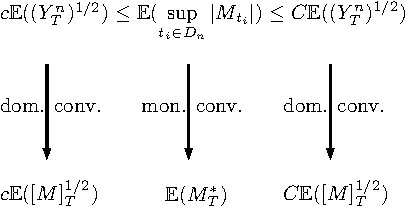
\includegraphics[scale=1.2]{conv.pdf}
\end{figure}
\end{proof}
Because $\mathcal{M}_{0, \text{loc}} = \mathcal{H}_{0, \text{loc}}^1$, we get as a direct consequence of Davis inequality
\begin{cor}\label{C38} If $M \in \mathcal{M}_{0, \text{loc}}$, then $[M]^{1/2}$ is locally integrable. 
\end{cor}
\newpage
\begin{defn} For $M \in \mathcal{M}_{0,\text{loc}},$ define $ \mathcal{L}^1(M)$ to be the space consisting of all predictable $H$ such that
\begin{align*}
\|H\|_{L^1(M)} := \EE \left[ \left( \int_0^T H_s^2 d[M]_s \right)^{1/2} \right] < \infty.
\end{align*}
Identifying $H, H'$ if $\|H-H'\|_{L^1(M)} =0$, yields space $L^1(M)$.  
\end{defn}
\begin{rem} \
\begin{enumerate}
\item Above definition is for $d=1$. For $d>1,$ $[M]$ is process with values in positive semidefinite $d\times d$-matrices, and 
\begin{align*}
\|H\|_{L^1 } = \EE \left[ \left( \int_0^T H_s^\text{tr} d[M]_sH_s \right)^{1/2} \right]. 
\end{align*}
\item If $M \in \mathcal{H}_0^1$, then $[M]^{1/2}$ is integrable and then $L^1 (M) \supset \pred:= \{$space of bounded predictable processes$\}$.
\item If $A$ is of FV, say $|A|$, define L$_\text{var}(A)$ as space of predictable $H$ with $\int_0^T |H_s| d |A|_s < \infty $ $\PP$-a.s. Notice that L$_\text{var}(A) \supset \pred_\text{loc}$. 
\end{enumerate}
\end{rem}
\begin{lem} \label{L39} If $M \in \mathcal{M}_{0, \text{loc}}$, then $\simple \cap L^1(M)$ is dense in $L^1(M)$ for $\| \cdot \|_{L^1(M)}. $
\end{lem}
\begin{proof}
By Corollary \ref{C38} we can take $\tau_m \nearrow T$ stationarily such that $( [M]^{\tau_m})^{1/2} = ([M^{\tau_m}])^{1/2}$ is integrable. If $H \in L^1(M)$, then 
\begin{align*}
H^m:= H1_{ [\![ 0, \tau_m]\!]} \to H \text{ in } L^1(M)
\end{align*}
and $H^m \in L^1( M^{\tau_m}).$ So w.l.o.g. assume $M \in \mathcal{H}_0^1$ and $H \in L^1(M)$. Then $H^k := h 1_{\{ |H| \leq k \}} \in \pred$ and $H^k \to H$ in $L^1(M)$ (by dominated convergence). \\
\\
Now suppose $M \in \mathcal{H}_0^1$ and $H \in \pred \subset L^1(M)$. Then we can find $H^j = \sum_k \lambda_k^j 1_{D_j^k}$ with $\lambda_k^j \in \mathbb{R}$, $D_j^k \in \mathcal{P}$ such that $\|H^j-H\|_\infty \to 0$ (and hence also in $L^1(M))$. Note however, that $H^j \notin \simple$ because $D_j^k \in \mathcal{P}$ does not need to be rectangular. \\
\\
But any $H$ of the form $H \lambda 1_D$ for $\lambda \in \mathbb{R}, D \in \mathcal{P}$ can be approximated in $L^1(M)$ by a sequence $(H^n)_{n \in \mathbb{N}} \subset \simple$ with $\|H^n\|_\infty \leq \|H\|_\infty = | \lambda|$. 
\begin{exe} Show that the claim in the previous phrase holds true by using a monotone class argument. 
\end{exe}
\noindent Putting all this together gives the result. 
\end{proof}
\newpage
We could now use Lemma \ref{L39} and completeness of $\mathcal{H}_0^1$ to exntend stochastic integrals for a local martingale, to $H \in L_\text{loc}^1(M)$ and in particular to $\pred_\text{loc}$. We want, however, a stronger continuity property and hence proceed differently. 
\begin{lem} \label{L310} Let $(M^n)_{n \in \mathbb{N}}, \ Y$ be martingales with $| \Delta M_\tau^n | \leq | \Delta Y_\tau |$ for all $n \in \mathbb{N}$ and for all stopping times $\tau$. If $\EE(1 \wedge [M^n]_T) \to 0$ i.e. $[M^n]_T \to 0$ in $L^0$, then $d_E' ( M^n,0 ) \to 0$. 
\end{lem}
\begin{proof}
Take $(H^n)_{n \in \mathbb{N}} \subset \simple_0$ with $\|H^n\|_\infty \leq 1$ and set $X^n:= H^n \cdot M^n$. Then $[X^n]_T \leq [M^n]_T \to 0$ in $L^0$, so that along a subsequence:
\begin{align*}
\PP([X^{n_k}]_T \geq 2^{-k}) \leq 2^{-k}, \text{ for all } k \in \mathbb{N}.
\end{align*}
By Borel-Cantelli $A:= \sum_{k=1}^\infty [X^{n_k}]$ is $\PP$-a.s. finite-valued and $[X^{n_k}]_T \to 0$ $\PP$-a.s. for $k \to \infty$. Let $\tau_m := \inf \{ t \in [0,T]: A_t \geq m \text{ or } |Y_t| \geq m \} \wedge T$ to get for all $k$
\begin{align*}
[X^{n_k}]_{\tau_m} \leq A_{\tau_m-} + ( \Delta X_{\tau_m}^{n_k})^2 \leq m + ( \Delta Y_{\tau_m})^2 \leq m + ((m+1) Y_{\tau_m}))^2.
\end{align*}
So we obtain $\sup_{k \in \mathbb{N}} ( [X^{n_k}]_{\tau_m})^{1/2} \in L^1$. Use now Theorem \ref{T37} and Lebesgue to get  
\begin{align*}
\EE( (X^{n_k})_{\tau_m}^*) \leq C \EE( [X^{n_k}]_{\tau_m}^{1/2}) \to 0 \text{ as } k \to \infty
\end{align*}
and of course $\PP( \tau_m = T) \to 1$ as $m \to \infty$. This implies that $(X^{n_k})_T^* = (H^{n_k} \cdot M^{n_k}) _T ^* \to 0$ in $L^0$ as $k \to \infty$. So every subsequence of $(H^n \cdot M^n)_{n \in \mathbb{N}}$ has a further subsequence which converges, uniformly on $[0,T]$, to $0$ in $L^0$. Thus the original sequence $(H^n \cdot M^n)_{n \in \mathbb{N}}$ already satisfies this convergence, and so we get 
\begin{align*}
\sup_{\substack{ H \in \simple_0 \\ \|H\|_\infty \leq 1}} \PP( (H \cdot M^n)_T^* \geq \epsilon) \xrightarrow{n \to \infty} 0, \text{ for all } \epsilon >0. 
\end{align*}
(If this fails, find sequence $(H^n)_{n \in \mathbb{N}}$ violating the above). We conclude that $d_E'(M^n,0) \to 0$ as $n \to \infty$. 
\end{proof}
\begin{cor}\label{C311} Let $M$ be a martingale and $(H^n)_{n \in \mathbb{N}} \subset \simple$ with $\|H^n\|_\infty \leq 1$. If $H^n \to 0$ pointwise, then $d_E' (H^n \cdot M, 0) \to 0$. 
\end{cor}
\begin{rem} The Lemma above gives a "nice and strong" convergence with respect to a "rich" topology.
\end{rem}
\begin{proof}
Let $M^n:= H^n \cdot M$ (which is a martingale) and $Y:= M$ to get $| \Delta M_\tau^n| = | H_\tau^n \Delta M_\tau | \leq | \Delta Y_\tau|$ for all $n \in \mathbb{N}$ and for all stopping times $\tau$. Moreover,
\begin{align*}
[M^n]_T = \underbrace{\int_0^T \underbrace{( H_s^n)^2}_{ \to 0, \text{ bdd. by $1$}} d[M]_s}_{ \text{bdd. by } [M]_T < \infty \ \PP\text{-a.s.}} \to 0 \ \PP\text{-a.s.}
\end{align*}
hence also in $L^0$. So Lemma \ref{L310} gives the desired conclusion.
\end{proof}
\newpage
\begin{thm}\label{T312} For any martingale $M \in \mathcal{H}_0^1$, the mapping $I_M( \simple, \| \cdot \|_\infty) \to ( \mathcal{S},  d_E')$ admits a unique linear extension to $J_M: \pred \to \mathcal{S}$ such that $H \cdot M := J_M(H)$ satisfies $[H \cdot M] = \int H^2 d [M]$ and $\Delta (H \cdot M) = H \Delta M$ and with dominated convergence property, i.e. that $(H^k) \subset \pred$ with $\|H^k\|_\infty \leq 1$ and $H^k \to 0$ pointwise implies $d_E'(H^k \cdot M, 0) \to 0$. Moreover, $J_M : ( \pred, \| \cdot \|_\infty) \to ( \mathcal{S}, d_E')$ is continuous. 
\end{thm}
\begin{proof}
Take $H \in \pred \subset L^1(M)$ and use Lemma $\ref{L39}$ to get $(H^n)_{n \in \mathbb{N}} \subset \simple$ with $\|H^n\|_\infty \leq \|H\|_\infty$ and $H^n \to H$ in $L^1(M)$-a.e. Then $H^n-H^m \to 0$ as $m,n \to \infty$ and hence $H^n-H^{m_n} \to 0$ as $n \to \infty$ for any $m_n \geq n$. So $d_E'((H^n-H^{m_n}) \cdot M, 0) \to 0$ as by Corollary \ref{C311} and so $d_E'(H^n \cdot M, H^m \cdot M) \to 0$ as $m,n \to \infty$. So $(H^n \cdot M)_{n \in \mathbb{N}}$ is Cauchy in $\mathcal{S}$ for $d_E'$, and so by Theorem \ref{T34} there exists limit in $\mathcal{S}$ for $d_E'$ and we define $H \cdot M:= d_E' \lim_{n \to \infty} H^n \cdot M$. \\
\\
Linearity, uniqueness are clear, and 
\begin{align*}
[H^n \cdot M] = \int(H^n) d[M], \ \Delta (H^n \cdot M) = H^n \Delta M, \text{ for all } n \in \mathbb{N}
\end{align*}
are easy because $H^n \in \simple.$ The result for $H$ then follows via limits. Dominated convergence property follows from Corollary \ref{C311} (plus its proof) for $M^k:= H^k \cdot M$ and continuity for $( \pred, \| \cdot \|_\infty)$ is then clear.
\end{proof}
Next we extend from $\mathcal{H}_0^1$-integrators to semimartingales $S$. If $S=A$ is of RV, we can define $H \cdot A = \int H_s dA_s$, for $H \in \pred \subset L_{\text{var}}(A)$ pathwise as usual Lebesgue-Stieltjes integral and check properties from known results. \\
\\
So we only need to argue for $S= M \in \mathcal{M}_{0, \text{loc}} = \mathcal{H}_{0, \text{loc}}^1$ and this is easy - use the following exercise: 
\begin{exe} $M^{\tau_m} \in \mathcal{H}_0^1$ for $\tau_m \nearrow T$ stationarily.
\end{exe}
One more localisation allows us to extend from $\pred$ to $\pred_\text{loc}$, and so $H \cdot S = \int H dS$ is well-defined and a semimartingale for any $S \in \mathcal{S}$ and any $H \in \pred_\text{loc}$.\\
\\
Now define on $\mathcal{S}$ two metrics 
\begin{align*}
\widetilde{d}_E(S^1,S^2)&:= \sup_{\substack{H \in \pred \\ \|H\|_\infty \leq 1}} \EE(1 \wedge |H \cdot (S^1-S^2)|_T) \geq d_E(S^1,S^2), \\
\widetilde{d}_E' (S^1,S^2)& := \sup_{ \substack{H \in \pred \\ \|H\|_\infty \leq1 }} \EE(1 \wedge (H \cdot (S^1-S^2))_T^*) \\
& \geq \max( d_E'(S^1,S`2), \widetilde{d}_E(S^1,S^2))
\end{align*}
Note that $\pred \supset \simple_0$. \newpage
One can argue as for Corollary \ref{C33} that $\widetilde{d}_E$ and $\widetilde{d}_E'$ are equivalent. Moreover, they are also equivalent to $d_E, d_E'$ (note that we already know that $d_E$ and $d_E'$ are equivalent). Indeed, $d_E' \leq \widetilde{d}_E'$ and for any $H \in \pred$ with $\|H\|_\infty \leq 1$, take $(H^n)_{n \in \mathbb{N}} \subset \simple$ with $\|H^n\|_\infty \leq 1$ and $H^n \to H$ a.e. Then write
\begin{align*}
\EE(1 \wedge | ( H \cdot (S^1-S^2))_T|) = d_{L^0} (H \cdot S_T^1, H \cdot S_T^2) \\
\leq d_{L^0} ( H \cdot S_T^1, H^n \cdot S_T^1) + d_{L^0} ( H^n \cdot (S_T^1-S_T^2) , 0) + d_{L^0} ( H^n \cdot S_T^1, H \cdot S_T^2) \\
 \leq d_E'((H-H^n) \cdot S_T^1) + d_E'( S^1, S^2) + d_E'( (H- H^n) \cdot S^2).
\end{align*}
Terms 1 and 3 converge to $0$ as $n \to \infty$ by the dominated convergence property (of Theorem \ref{T312}) and so taking sup over all $H \in \pred, \ \|H\|_\infty \leq 1$ gives $\widetilde{d}_E \leq d_E'$. This is enough. 
\\
\\
\textbf{Terminology}: $\widetilde{d}_E'$ ("strongest") is \textbf{Emery metric} on $\mathcal{S}$ and corresponding (metric) topology is \textbf{Emery topology}.
\\\\
We summarize our knowledge in the next theorem:
\begin{thm}\label{T313} For every semimartingale $S$ and every $H \in \pred$ stochastic integral $H \cdot S= \int H dS$ is well-defined and a semimartingale. Moreover  the mapping 
\begin{align*}
\begin{cases} ( \pred \times \mathcal{S}, \| \cdot \|_\infty \times \widetilde{d}_E') & \longrightarrow ( \mathcal{S}, \widetilde{d}_E') \\
(H, S) & \longmapsto H \cdot S
 \end{cases}
\end{align*}
is continuous. 
\end{thm}
\begin{proof}
Take $(H^n)_{n \in \mathbb{N}} \subset \pred$ with $\|H^n-H\|_\infty \to 0$ and $(S^n) \subset \mathcal{S}$ with $\widetilde{d}_E'(S^n,S) \to 0$. Then  
\begin{align*}
\widetilde{d}_E'(H^n \cdot S^n, H \cdot S) &\leq \widetilde{d}_E'(H^n \cdot S^n , H^n \cdot S) + \widetilde{d}_E'(H^n \cdot S, H \cdot S) \\
& = \sup_{ \substack{ K \in \pred \\ \|K\|_\infty \leq 1}} \EE(1 \wedge ((KH^n) \cdot (S^n-S))_T^*) + \widetilde{d}_E'((H^n-H) \cdot S, 0).
\end{align*}
The second term vanishes by dominated convergence property, and the first time goes to $0$ by definition of $\widetilde{d}_E'$ because $d_E'(S^n-S, 0) \to 0$ as $n \to \infty$ (uses $\|H^\|_\infty \leq 1)$. 
\end{proof}
\newpage
In Theorem \ref{T312} we have $H \cdot M$ for $M \in \mathcal{H}_0^1$ and $H \in \pred$. \textbf{But}: construction as limit in $\mathcal{S}$, so that  
\begin{align*}
H \cdot M = \int H dM \text{ is in } \mathcal{S}.
\end{align*}
Is $H \cdot M$ a martingale? More subtle than it looks: If $M$ is a martingale and $H$ is bounded, predictable, then $H \cdot M$ is a semimartingale - but it can fail to be a martingale (unlike in discrete time! striking difference here!) Counterexamples in Herdegem/Herrimann, in continuous time. Nevertheless, we have:
\begin{prop} \label{P314} If $M \in \mathcal{H}_0^1$ and $H \in \pred$, then $H \cdot M \in \mathcal{H}_0^1$. 
\end{prop}
\begin{proof}
As in Lemma \ref{L39}, take $(H^n)_{n \in \mathbb{N}} \subset \pred$ with $\|H^n\|_\infty \leq \|H\|_\infty$ and $H^n \to H$ $L^1(M)$ a.e. Then by Theorem \ref{T312}, $H^n \cdot M \to H \cdot M$ for $d_E'$. But better: by Theorem \ref{T37} (Davis inequality), $[M]_T^{1/2} \in L^1$ and so by Lebesgue dominated convergence 
\begin{align*}
\EE \left[ \left( \int_0^T (H_s^n-H_s)^2 d [M]_s \right)^{1/2} \right] \xrightarrow{n \to \infty} 0. 
\end{align*}
Again by Theorem \ref{T37} $(H^n \cdot M)_{n \in \mathbb{N}}$ is Cauchy for $\| \cdot \|_{ \mathcal{H}_0^1 }$, and so the limit is again $\mathcal{H}_0^1$. 
\end{proof}
Now comes the final extension of integrands (most general case). 
\begin{defn} Fix a semimartingale $S$. A predictable process $H$ is \textbf{$S$-integrable}, denoted as $H \in \mathcal{L}(S)$, if $(H^n \cdot S)_{n \in \mathbb{N}}$ is Cauchy in Emery topology (or for $d_E'$), where $H^n:= H 1_{\{ |H| \leq n\}} \in \pred$. Limit in $\mathcal{S}$ is called $H \cdot S$. 
\end{defn}
\begin{rem} \label{rem1} If $H,H'$ are in $\mathcal{L}(S)$ with $|H| \leq |H'|$, then $\widetilde{d}_E'(H \cdot S, 0) \leq \widetilde{d}_E'(H' \cdot S, 0)$. Indeed, $ \{ H \neq 0 \} \subset \{ H' \neq 0 \}$ implies for any $J \in \pred$ with $\|J\|_\infty \leq 1$, 
\begin{align*}
J \cdot (H \cdot S)= (JH) \cdot S = (JH 1_{\{ H \neq 0\}}) \cdot S =  \left( J \frac{H}{H'}1_{\{ H \neq 0 \}} H' \right) \cdot S = K \cdot (H' \cdot S),
\end{align*}
where $K:= J H/H' 1_{\{ H \neq 0\}} \in \pred$ with $\|K \|_\infty \leq 1$ due to $|H| \leq |H'|$. So definition of $\widetilde{d}_E'$ gives the desired result.
\end{rem}
\begin{rem}Some arguments above and in what follows assume $d=1$. If $H$ and $S$ are $\mathbb{R}^d$-valued, then $H \cdot S$ is $\mathbb{R}$-valued, but e.g. $[S]$ is $\mathbb{R}^{d \times d}$-valued and $[H \cdot S] = \int H^\text{tr} d[S]H.$ Moreover, $H \cdot S$ can be well defined even if not all $H^i \cdot S^i$ are. For details, see Cherny/Shiryaev. 
\end{rem}
\newpage
The next Proposition gives a characterisation of $\mathcal{L}(S)$. 
\begin{prop} \label{P315} Suppose $S$ is a semimartingale and $H$ is predictable. Then $H \in \mathcal{L}(S)$ iff for all sequences $(K^n)_{n \in \mathbb{N}} \subset \pred$ with $|K^n| \leq |H|$ and $K^n \to 0$ pointwise, we have $\widetilde{d}_E'(K^n \cdot S,0) \to 0$. 
\end{prop}
\begin{rem} This includes a dominated convergence property on $\pred$ with bound in $\mathcal{L}(S) \supset_{\neq} \pred$. 
\end{rem}
\begin{proof}
"$\implies$" Let $H^n:= H 1_{\{ |H| \leq n\}}$. Then $(H^n \cdot S)_{n \in \mathbb{N}}$ is Cauchy for $\widetilde{d}_E'$ and so 
\begin{align*}
\widetilde{d}_E' ((H 1_{\{ |H| > n \}}) \cdot S) = \widetilde{d}_E' (H \cdot S, H^n  \cdot S) \to 0.
\end{align*}
In consequence, by remark \ref{rem1}, $\widetilde{d}_E'((K^n 1_{\{ | H| > n\}} ) \cdot S, 0) \to 0$. Take $m \neq n$ and write  
\begin{align*}
(K^n 1_{\{ |H| \leq n\}} ) \cdot S = (K^n 1_{\{ |H| \leq n\}}) \cdot S + (K^n 1_{\{ m < |H| \leq n \}}) \cdot S.
\end{align*}
Recall $|K^n| \leq |H|$. For fixed $m$, the first term converges to $0$ for $\tilde{d}_E'$ by usual dominated convergence property for $\pred$. Next, 
\begin{align*}
\widetilde{d}_E' ( 2. \text{ term},0) \overset{\text{Rem \ref{rem1}}}\leq \widetilde{d}_E' (H 1_{\{ m < |H| \leq n \}} ) \cdot S, 0) = \widetilde{d}_E' (H^n \cdot S, H^m \cdot S) \xrightarrow{n,m \to \infty} 0
\end{align*}
by the Cauchy property. So we get $\widetilde{d}_E'((K^n 1_{\{ |H| \leq n\}}) \cdot S, 0) \to 0$ and hence \\ $\widetilde{d}_E' (K^n \cdot S, 0) \to 0$.  \\
\\
"$\Longleftarrow$" For any $m_n \geq n$, define $K^n:= H^{m_n}-H^n= H 1_{\{ n < |H| \leq m_n\}}$. So $|K^n| \leq |H|$ and $K^n \to 0$. So   
\begin{align*}
\widetilde{d}_E' ( H^{m_n} \cdot S, H^n \cdot S) = \widetilde{d}_E' ( K^n \cdot S, 0 ) \xrightarrow{n \to \infty} 0
\end{align*}
and as $m_n \geq n$ was arbitrary, we get $\widetilde{d}_E'(H^m \cdot S, H^n \cdot S) \to 0$ as $m,n \to \infty$. This is the Cauchy property for $(H^n \cdot S)_{n \in \mathbb{N}}$ and so $H \in \mathcal{L}(S)$. 
\end{proof}
Later, we need for the space of all stochastic integrals $\{ H \cdot S : H \in \mathcal{L}(S) \}$ closedness result: Fix $S$ and define $d_S(H,H'):= \widetilde{d}_E'(H \cdot S , H \cdot S')$ for $H,H' \in \mathcal{L}(S)$, so integrands are close for $d_s$ iff their stochastic integrals are close for Emery metric. 
\\\\
Identify $H, H'$ if $d_S(H,H')=0$ (gives equivalence classes) resulting space $L(S)$ is then metric space with metric $d_S$. 
\newpage
\begin{thm}[Mémin] \label{T317} Let $S=(S_t)_{0 \leq t \leq T}$ be a $\mathbb{R}^d$-valued semimartingale. Then $(L(S), d_S)$ is a complete metric space. Equivalently, space of all stochastic integrals of $S$ 
\begin{align*}
\left\{ X= \int H dS = H \cdot S, H \in L(S) \right\}
\end{align*}
is closed for Emery topology (i.e. for $\widetilde{d}_E')$. 
\end{thm}
\begin{rem} We have seen in IMF that in \textbf{finite discrete} time, the space of all \textbf{final values} of stochastic integrals 
\begin{align*}
G_T( \Theta) = \{ G_T( \vartheta) : \vartheta \in \Theta\} = \left\{ \int_0^T \vartheta_u dS_u : \vartheta \ \mathbb{R}^d\text{-valued predictable} \right\} \subset L^0
\end{align*}
is closed in $L^0$. So we can ask: Is in general $\{ H \cdot S_T : H \in L(S) \}$ closed in $L^0$? 
\\
This is \textbf{not true} - in general, unlike in finite discrete time, a control on \textbf{final value} $H \cdot S_T$ does not give any control on the process $H \cdot S$, and so we cannot work. 
\end{rem}
Before we prove Theorem \ref{T317} we need an auxiliary result:
\begin{lem}\label{L316} Suppose $( \gamma_k)_{k \in \mathbb{N}} \subset \pred$ satisfy $\sum_{k=1}^\infty d_s( \gamma_k,0) < \infty$ and define $[0,+ \infty]$-valued process $G:= \sum_{k=1}^\infty | \gamma_k|$. Then 
\begin{enumerate}
\item For each $t \in [0,T]$, $ \{ \int_0^t H_u dS_u : H \in \pred , |H| \leq G \}$ is bounded in $L^0$. 
\item If $(K^n)_{n \in \mathbb{N}} \subset \pred$ satisfies $K^n \to 0$ pointwise and $|K^n| \leq G$, then \\ $\widetilde{d}_E'( K^n \cdot S,0) \to 0$. 
\begin{itemize}
\item Does not follow from Proposition \ref{P315} because maybe $G \notin \mathcal{L}(S)$.
\end{itemize}
\item For any $H \in \pred$, $ \int H 1_{\{ G = \infty\}} dS =0$. 
\end{enumerate}
\end{lem}
\begin{proof}
We start with general considerations. Take $K \in \pred$ with $|K | \leq G$, set 
\begin{align*}
G^m:= \sum_{k=1}^m | \gamma_k| \nearrow G \text{ and } K^m:= (K \wedge G^m) \vee (- G^m).
\end{align*}
Then $|K^m| \leq |K| \in \pred$ and $K^m \to K$ pointwise,  so that $d_S( \lambda K^m,0) \to d_S( \lambda K,0)$ as $m \to \infty$ for any $\lambda \geq 0$, by Theorem \ref{T312} (dominated convergence property). Moreoever, $|K^m| \leq \sum_{k=1}^m ( |K| \wedge | \gamma^k|)$ implies for fixed $\lambda >0$, that 
\begin{align*}
d_S( \lambda K,0) = \lim_{m \to 0} d_S( \lambda K^m, 0) \leq \lim_{m \to \infty} \sum_{k=1}^m d_S( \lambda  (|K| \wedge |\gamma_k|),0) =  \sum_{k=1}^m d_S( \lambda ( |K| \wedge | \gamma_k|,0).
\end{align*}
\newpage
We can take $( \lambda_n) \subset [0,1]$ and $(K^n)_{n \in \mathbb{N}} \subset \pred$ to get analogous estimate for $d_S( \lambda_n K^n,0)$. If $\lambda_n \to 0$ or $K^n \to 0$ pointwise, then for each $k \in \mathbb{N}$ we have $\lim_{n \to \infty} d_S( \lambda_n ( |K^n| \wedge | \gamma_k|),0)=0$  by Theorem \ref{T312}. 
\\\\
Moreover, $d_S( \lambda_n( |K^n| \wedge | \gamma_k|,0) \leq d_S( \gamma_k,0)$ which is summable over $k \in \mathbb{N}$ by assumption, so applying Lebesgue dominated convergence to the sum above yields
\begin{align*}
\lim_{n \to \infty} d_S( \lambda_n K^n,0) &\leq \lim_{n \to \infty} \sum_{k=1}^\infty d_S( \lambda ( |K^n| \wedge | \lambda_k|,0) \\ &\overset{\text{Lebesgue}}= \sum_{k=0}^\infty \lim_{n \to \infty} d_S( \lambda_n ( |K^n| \wedge | \lambda_k|),0) =0, \text{ if } \begin{cases} \lambda_n \xrightarrow{\text{pointwise}} 0 \\ \text{or} \\ K^n \xrightarrow{\text{pointwise}} 0 \end{cases}
\end{align*}
We will now use the above derived general result, in order to conclude 1)-3).
\\
\\
1) Take any $(K^n)_{n \in \mathbb{N}} \subset \pred$ with $|K^n| \leq G$ and $\lambda_n \to 0$. Then $\lambda_n \int_0^t K_u^n dS_u \to 0$ in $L^0$, for each $t \in \mathbb{R}_+$ 
\begin{exe} The setting as in 1) above ensures that 
\begin{align*}
\left\{ \int_0^t K_u dS_u : K \in \pred , |K | \leq G \right\} \text{ is bounded in } L^0.
\end{align*}
\end{exe}
\noindent 2) Take $\lambda_n \equiv 1$. Then by definition 
\begin{align*}
\widetilde{d}_E'( K^n \cdot S, 0) = d_S(K^n,0) \to 0. 
\end{align*}
3) $G$ is predictable, and so $H1_{\{ G = \infty\}} \in \pred$ if $H \in \pred$. For $c_n \to 0$, $H^n:= c_n H 1_{\{ G = \infty\}}$ satisfies $|H^n| \leq |G|$ because $G= \infty$ on $\{ G= \infty\}$. By 1) we get 
\begin{align*}
\left( c_n \int_0^t H_u 1_{\{ G= \infty\}} dS_u \right)_{n \in \mathbb{N}} \text{ is bounded in } L^0.
\end{align*}
This is only possible if $\int_0^t H_u 1_{\{ G= \infty\}} dS_u =0$ and $t$ was arbitrary. 
\end{proof}
\newpage
\begin{proof}[Proof of Theorem \ref{T317}] Equivalence is clear from the definition of $d_S$ from $\widetilde{d}_E'$ and the fact that $( \mathcal{S}, \widetilde{d}_E')$ is complete. \\
\\
Take $(\widetilde{H}^n)_{n \in \mathbb{N}} \subset L(S)$ which is Cauchy for $d_S$. We need to show that there exists $\widetilde{H} \in L(S)$ with $d_S( \widetilde{H}^n, \widetilde{H}) \to 0$. Approximate each $\widetilde{H}^n$ by $H^n \in \pred$ (use definition of $L(S)$ and $d_S$) in $d_S$. Choose subsequence, again called $(H^n)_{n \in \mathbb{N}}$, with $d_S(H^n, H^{n-1}) \leq 2^{-n}$ (using Cauchy property plus $H^n \approx \widetilde{H}^n$). Then it is enough to find some $H \in L(S)$ with $H^n \cdot S \to H \cdot S$ for $\widetilde{d}_E'$. \\
\\
Define $\gamma_n := H^{n+1}-H^n \in \pred$ and $G:= \sum_{n=1}^\infty | \gamma_n|$. For any $(K^n)_{n \in \mathbb{N}} \subset \pred$ with $|K^n| \leq G1_{\{ G < \infty \}}$ and $K^n \to 0$, we get $\widetilde{d}_E'(K^n \cdot S,0) \to 0$ by Lemma \ref{L316}, 2). So $G1_{\{ G < \infty \}} \in L(S)$ by Proposition \ref{P315} on $\{G < \infty\}$. \\
\\
$\overline{H}:= \sum_{n=1}^\infty \gamma_n = \sum_{n=1}^\infty (H^{n+1}-H^n)$ is well-defined and $\overline{H}1_{\{ G < \infty\}}$ is predictable with $| \overline{H} 1_{\{ G < \infty\}} | \leq G$. So we can first use (for any test $(K^n)_{n \in \mathbb{N}}$) Lemma \ref{L316} 2) and then again Proposition \ref{P315} to obtain that $\overline{H}1_{\{ G < \infty\}}$ is in $L(S)$. So is then $H:= (\overline{H}+H^1)1_{\{ G < \infty\}}$ because $H^1 \in \pred \subset L(S)$. \\
\\
But $H^1 + \overline{H}-H^n = \sum_{k=n}^\infty \gamma_k$ implies that 
\begin{align*}
d_S(H, H^n 1_{\{ G < \infty\}}) \leq \sum_{k=n}^\infty d_S( \gamma_k,0) \xrightarrow{n \to \infty} 0,
\end{align*}
because $\sum_{k=1}^\infty d_S( \gamma_k, 0) < \infty$.  Finally, $H^n \in \pred$, so by Lemma \ref{L316} 3) 
\begin{align*}
\int H^n 1_{\{ G < \infty\}} dS = H^n \cdot S
\end{align*}
and thus 
\begin{align*}
\widetilde{d}_E' ( H \cdot S, H^n \cdot S) = d_S( H, H^n) \xrightarrow{n \to \infty} 0
\end{align*}
and so we have found our $H$. 
\end{proof}
\newpage
\section{The fundamental theorem of asset pricing (FTAP)}
\textbf{Goal}: Precise formulation for equivalence between "absence of arbitrage" and "existence of an EMM" in general continuous time model. 
\\\\
\textbf{Setup}: $( \Omega, \mathcal{F}, \mathbb{F}, \PP)$ with $\mathbb{F}= ( \mathcal{F}_t)_{0 \leq t \leq T}$ satisfying the usual conditions. Moreover, $B=1$, $S$ adapted RCLL $\mathbb{R}^d$-valued and also assume $S$ is a \textbf{semimartingale}.\\
\\
Recall space $L(S)$ of $\mathbb{R}^d$-valued predictable $S$-integrable $\vartheta$, define $G( \vartheta):= \int \vartheta dS = \vartheta \cdot S$, and call $\vartheta$ \textbf{$a$-admissible} for $a \geq 0$ if $G_\cdot ( \vartheta) \geq -a \ \PP$-a.s. Call $\Theta^a$ all $a$-admissible $\vartheta \in L(S)$, $\Theta_\text{adm} = \cup_{a \geq 0 } \Theta^a$ and introduce 
\begin{align*}
\mathcal{G}^a &:= G_T( \Theta^a) = \left\{ G_T( \vartheta) = \int_0^T \vartheta_u dS_u : \vartheta \in \Theta^a \right\} \\
\mathcal{G}_\text{adm}&:= G_T( \Theta_\text{adm}) = \bigcup_{a \geq 0} \mathcal{G}^a.
\end{align*}
\textbf{Interpretation}: any $g \in \mathcal{G}^A$ represents the final wealth of some self-financing trading strategy $\varphi \teq ( 0, \vartheta)$ starting from $0$ initial wealth and with wealth bounded from below by $-a$. 
\\
\\
\textbf{No arbitrage}: (NA) is defined to be the condition $\mathcal{G}_\text{adm} \cap L_+^0 = \{0 \}$.
\\\\
Recall that $Q \approx \PP$ is an ELMM for $S$ if $S \in \mathcal{M}_\text{loc}(Q)$. The next Lemma we've already discussed in section 2, we now have the tools to rigorously prove it. 
\begin{lem}\label{L41} Suppose $S$ is adapted RCLL. If $S$ admits an ELMM, say $Q$, then $S$ satisfies (NA), i.e. $G_T( \Theta_\text{adm}) \cap L_+^0 = \{0 \}$. 
\end{lem}
For a complete proof, we need an auxiliary result: 
\begin{prop}[Ansel-Stricker] \label{P41} Suppose $M$ is a local martingale and $\vartheta \in L(M)$. If $\int \vartheta dM \geq -b$ for some $b \geq 0$, then also $\int \vartheta dM$ is a local martingale and a supermartingale. 
\end{prop}
We first prove a more general result, due to De Donno/Pratelli.
\begin{lem} \label{L42} Suppose $X$ is adapted RCLL. Let $( \gamma_n)_{n \in \mathbb{N}} \subset L^1$ and $( \tau_n)_{n \in \mathbb{N}}$ a localising sequence (increasing to $T$ stationarily) be such that $X^{\tau_n} \geq \gamma_n$ for all $n \in \mathbb{N}$. Let $(M^n)_{n \in \mathbb{N}}$ be a sequence of martingales with $d(M^n,X) \to 0$ as $n \to \infty$ (i.e. $M^n \to X$ uniformly in $t \in [0,T]$ in $L^0$) and $( \Delta M_\sigma^n)^\pm \leq ( \Delta X_\sigma)^\pm$ for all $n \in \mathbb{N}$ and for all stopping times $\sigma$. Then $X$ is a local martingale. 
\end{lem}
\newpage
\begin{proof}
\textbf{Idea}: Construct a good sequence $(\sigma_m)_{m \in \mathbb{N}}$ of stopping times, then $M_{t \wedge \sigma_m}^n \xrightarrow{n \to \infty} X_{t \wedge \sigma_m}$ in $L^0$ for all $m \in \mathbb{N}$, argue that convergence even takes place in $L^1$ and that $X_{t \wedge \sigma_m} \in L^1$. Then $X^{\sigma_m}$ is a martingale, i.e. $X$ is a local martingale. 
\\\\
Assume $M_0^n \equiv X_0 =0$. Define stopping times 
\begin{align*}
\rho_n := \inf \{ t \in [0,T]: X_t >n \text{ or } M_t^n > X_t+1 \text{ or } M_t^n < X_t-1 \} \wedge T.
\end{align*}
By passing to a subsequence, we may assume that $\sum_{n=1}^\infty \PP( \rho_n < T)  <\infty$. Then $\PP( \inf_{n \geq m} \rho_n =T) \xrightarrow{m \to \infty} 1$ because 
\begin{align*}
\PP( \inf_{n \geq m} \rho_n = T)= 1- \PP \left( \bigcup_{n \geq m } \{ \rho_n < T \} \right) \geq 1 - \underbrace{\sum_{n = m}^\infty \PP( \rho_n < T)}_{ \xrightarrow{m \to \infty}0 } \xrightarrow{m \to \infty} 1.
\end{align*}
Thus $\sigma_m := \tau_m \wedge \inf_{n \geq m} \rho_n \nearrow T$ stationarily as $m \to \infty$. 
\\\\
\textbf{Claim}: $X^{\sigma_m}$ is a martingale. 
\\\\
To see this, start with 
\begin{align*}
( \Delta M_{t \wedge \sigma_m}^n)^- \leq ( \Delta X_{t \wedge \sigma_m})^- \overset{X^{\tau_m} \geq \gamma_m, X_{\rho_m^-} \leq m } \leq m- \gamma_m.
\end{align*}
Moreover, for $n \geq m$ and $t < \sigma_m$, we have $M_{t \wedge \sigma_m}^n = M_t^n \geq X_t-1 \geq \gamma-1$, and so for all $n \geq m$ and all $t \in \mathbb{R}_0^+$, $M_{t \wedge \sigma_m}^n \geq \gamma_m-1-(m-\gamma_m) \in L^1$. So we obtain 
\begin{align*}
\EE( X_{t \wedge \sigma_m}) = \EE( \lim_{n \to \infty} M_{t \wedge \sigma_m}^n) \overset{\text{Fatou}} \leq \liminf_{n \to \infty} \underbrace{\EE( M_{t \wedge \sigma_m}^n)}_{=0,\ (\text{mart.})}=0
\end{align*}
and $X_{t \wedge \sigma_m}^- \in L^1$ because $X_{t \wedge \sigma_m} \geq \gamma_m \in L^1$. Hence $\EE( X_{t \wedge \sigma_m}^+) \leq \EE( X_{t \wedge \sigma_m}^-) < \infty$ and so $X_{t \wedge \sigma_m} \in L^1$ for all $t$. Then also $\Delta X_{t \wedge \sigma_m} \in L^1$ because $X_{( t \wedge \sigma_m)^-} \leq m$.  \\
By an analog argument, we get 
\begin{align*}
M_{t \wedge \sigma_m}^n \leq m+1 + ( \Delta M_{t \wedge \sigma_m}^n)^+ \leq m+1 + | \Delta X_{t \wedge \sigma_m}| \in L^1, \text{ for all } n \in \mathbb{N}.
\end{align*}
Moreover, $M_{t \wedge \sigma_m}^n \xrightarrow{n \to \infty} X_{t \wedge \sigma_m}$ in $L^0$, hence in $L^1$ and so $X^{\sigma_m}$ is a martingale because all $(M^n)^{\sigma_m}$ are. 
\end{proof}
\newpage
\begin{proof}[Proof of Proposition \ref{P41}] Since $\mathcal{M}_{0, \text{loc}} = \mathcal{H}_{0, \text{loc}}^1$ allows us by stopping to assume that $M \in \mathcal{H}^1$. Take $\vartheta \in L(M)$ and $\vartheta_\cdot^n := \vartheta_\cdot 1_{\{ | \vartheta \leq n \}}$ and set $M^n:= \int \vartheta^n d M$. By definition, $M^n \to \int \vartheta dM =: X$ for Emery metric $\widetilde{d}_E' \geq d$, and each $M^n \in \mathcal{H}^1$ by Proposition \ref{P314}. Because $X \geq -b$, all assumptions of Lemma \ref{L42} are satisfied and so $X= \int \vartheta dM$ is a local martingale. Moreover, as $X \geq -b$ it is also a supermartingale by Fatou. 
\end{proof}
\begin{rem} From the proof above: conclusion still holds if instead of $\int \vartheta dM \geq -b$, we only have that all large jumps of $\int \vartheta dM$ (say $\geq C$) have lower bounded in $L^1$. 
\end{rem}
We now prove Lemma \ref{L41}
\begin{proof}[Proof of Lemma \ref{L41}] We first argue that $S$ is a $\PP$-semimartingale: Indeed, by Theorem \ref{T25} and Theorem \ref{T27} semimartingales are the same as good integrators and like $L^0$, this concept is the same for $\PP$ and for any $R \approx \PP$. Now $S \in \mathcal{M}_\text{loc}(Q)$, so $S$ is a $Q$-seminmartingale and as $Q \approx \PP$, $S$ is also a $\PP$-seminmartingale. So $L(S)$, $\Theta_\text{adm}$ (NA) all make sense under $\PP$. 
\\\\
Suppose $\vartheta \in \Theta_\text{adm}$. Then $ \int \vartheta dS \geq$ constant a.s. and $S \in \mathcal{M}_\text{loc}(Q)$; so $\int \vartheta dS$ is a $Q$-local martingale and $Q$-supermartingale by Proposition \ref{P41} (Ansel-Stricker). Hence $\EE_Q(G_T( \vartheta)) \leq 0$, if also $G_T( \vartheta) \in L_+^0$, i.e. nonnegative a.s., we must have that $G_T( \vartheta)=0$ a.s. and so we get (NA).
\end{proof}
So, the existence of a ELMM $\implies $(NA), and we have seen from counterexample that $\centernot\Longleftarrow$. So we need to strengthen (NA). 
\\\\
\textbf{Recall}: $\mathcal{C}^\infty := ( G_T( \Theta_\text{adm})-L_+^0) \cap L^\infty$ is set of all bounded payoffs which can be dominated/superreplicated by final wealth of some admissible self-financing strategy with $0$ initial wealth. 
\begin{exe} (NA) $\mathcal{G}_T( \Theta_\text{adm}) \cap L_+^0 = \{0\}$ is equivalent to (NA) $\mathcal{C}^\infty \cap L_+^\infty = \{0 \}$. 
\end{exe}
\begin{mdframed}[backgroundcolor=yellow!20, topline=true, linewidth=2.0pt]
\begin{defn}
A semimartingale $S=(S_t)_{0 \leq t \leq T}$ satisfies \textbf{no free lunch with vanishing risk} if 
\begin{itemize}
\item (NFLVR): $\overline{\mathcal{C}^\infty}^{L^\infty} \cap L_+^\infty = \{0 \}$. 
\end{itemize}
where $\overline{\cdot}^{L^\infty}$ is (norm) closure in $L^\infty$. 
\end{defn}
\end{mdframed}
\newpage
\begin{rem} \ \begin{itemize}
\item By definition, (NFLVR) $\implies$ (NA). Moreover, (NFLVR) forbids not only, like (NA), generating profits directly from $0$, but also asymptotically (i.e. as limits in $L^\infty$).
\item Later, we want to use Kreps-Yan theorem, for $p= \infty$. Then we need to use on $L^\infty$ weak* topology $\sigma( L^\infty, L^1)$ and we have $\overline{\cdot}^{L^\infty} \subset \overline{\cdot}^{\sigma(L^\infty, L^1)}$. We also need in Kreps-Yan theorem closedness for $\sigma(L^\infty, L^1)$. On economic grounds, using in (NFLVR) $\overline{\cdot}^{L^\infty}$ is much more natural than it would be using $\overline{\cdot}^{\sigma(L^\infty, L^1)}$ (NFL). This is at the root of later technical difficulties. 
\end{itemize}
\end{rem}
\begin{prop} \label{P43} For a semimartingale $S=(S_t)_{0 \leq t \leq T}$ the following are equivalent: 
\begin{enumerate}
\item $S$ satisfies (NFLVR) 
\item Any sequence $g_n= G_T( \vartheta^n)$ in $\mathcal{G}_\text{adm}$ for $n \in \mathbb{N}$ with $G_T^-( \vartheta^n) \to 0$ in $L^\infty$ converges to $0$ in $L^0$.
\begin{itemize}
\item That is, if losses go to $0$ uniformly, then wealth or gains go to $0$ in $L^0$. 
\end{itemize}
\item $S$ satisfies (NA) plus \textbf{no unbounded profit with bounded risk}, \\
(NUPBR): $\mathcal{G}^1 = G_T( \Theta^1)= \{ G_T( \vartheta): \vartheta \text{ is $1$-admissible}\}$ is bounded in $L^0$ (i.e. $\sup_{g \in \mathcal{G}^1} \PP( |g| \geq n) \to 0$ as $n \to \infty$).
\end{enumerate}
\end{prop}
\begin{rem} In brief: (NFLVR)=(NA)+(NUPBR).
\end{rem}
\begin{proof}
"2)$\implies$3)": Any $f \in \mathcal{C}^\infty \cap L_+^\infty$ has form $0 \leq f= g-Y$ with $g \in G_T( \Theta_\text{adm})$, $Y \geq 0$. So $g \geq 0$ and by taking $g_n \equiv g$ in 2) gives $g \equiv 0$ and thus $f \equiv 0$, so we have (NA). \\
\\
If (NUPBR) fails, then $\mathcal{G}^1$ is not bounded in $L^0$ and so there exists $ \gamma_n \nearrow + \infty$ with $\PP(g_n \geq \gamma_n) \geq \delta >0$ for some sequence $(g_n)_{n \in \mathbb{N}} \subset \mathcal{G}^1$. But $g_n = G_T( \vartheta^n)$ with $\vartheta^n$ $1$-admissible means that  
\begin{align*}
\widetilde{g}_n:= \frac{1}{\gamma_n}g_n
\end{align*}
is in $\mathcal{G}_\text{adm}$ with $\widetilde{g}_n^- \to 0$ in $L^\infty$ because $\| \widetilde{g}_n \|_{L^\infty} \leq \frac{1}{\gamma_n}$. \\ But we also have $\PP( \widetilde{g}_n \geq 1) = \PP(g_n \geq \gamma_n) \centernot\to 0$, so $\widetilde{g}_n \centernot\to 0$ in $L^0$ and this contradicts 2). 
\newpage
In order to continue the proof we need an auxiliary result from probability theory which is extremely useful
\begin{lem}\label{L44} For any sequence $(X_n)_{n \in \mathbb{N}} \subset L_+^0$, there exists convex combinations $\widetilde{X}_n \in \text{conv}(X_n,X_{n+1}, \dots )$, $n \in \mathbb{N}$ such that $(\widetilde{X}_n)_{n \in \mathbb{N}}$ converges $\PP$-a.s. to some $\widetilde{X}_\infty$ taking values in $[0, + \infty]$. Moreover, if $\PP( X_n \geq \alpha) \geq \delta > 0$ for some $\alpha >0$, then $\PP( \widetilde{X}_\infty >0 ) >0$. If conv($X_1, X_2, \dots )$ is bounded in $L^0$, then $\widetilde{X}_\infty < \infty$ $\PP$-a.s. 
\end{lem}
For a proof of Lemma \ref{L44} see Appendix B.
\\
\\
"3)$\implies$1)": Suppose (NA) holds but (NFLVR) fails, then we claim that (NUPBR) fails as well and the result follows. To see this: (NFLVR) fails means there exists a sequence $(f_n)_{n \in \mathbb{N}} \subset \mathcal{C}^\infty$ and $f \in L_+^\infty \setminus \{0\}$ with $\|f-f_n\|_\infty \leq \frac{1}{n}$. \\
\\
Now $f_n \leq g_n$ for some $g_n \in \mathcal{G}_\text{adm}$ (by Definition of $\mathcal{C}^\infty$), so $\|g_n^-\|_\infty \leq \|f_n^-\|_\infty \leq \frac{1}{n},$ and due to (NA), $g_n = G_T( \vartheta^n)$ with $\vartheta^n \in \Theta_\text{adm}$ and $g_n \geq - \frac{1}{n}$ implies that $G_\cdot ( \vartheta^n) \geq - \frac{1}{n}$. 
\begin{exe} Verify that the statement in the previous paragraph holds.
\end{exe}
\noindent This means that $n \vartheta^n$ is $1$-admissible and so $n g_n \in \mathcal{G}^1$. Using Lemma \ref{L44} gives $\widetilde{g}_n \in \text{conv}(g_n, g_{n+1}, \dots )$ with $\widetilde{g}_n \to \widetilde{g}_\infty \ \PP$-a.s., and $g_n \geq f_n$ gives $\widetilde{g}_\infty \geq f$ so that $\PP( \widetilde{g}_\infty > 0)>0$. But now $(n \widetilde{g}_n)_{n \in \mathbb{N}} \subset \mathcal{G}^1$ has $\frac{1}{n}n \widetilde{g}_n = \widetilde{g}_n$ not converging to $0$ in $L^0$. So $\mathcal{G}^1$ is not bounded in $L^0$ and thus (NUPBR) fails. 
\\\\
"1)$\implies$2)": Take $(g_n)_{n \in \mathbb{N}} \subset \mathcal{G}_\text{adm}$ with $g_n^- \to 0$ in $L^\infty$ and suppose $g_n \centernot\to 0$ in $L^0$. Then along a subsequence, again called $(g_n)_{n \in \mathbb{N}}$, we get $\PP( g_n \geq \alpha) \geq \delta >0$ for some $\alpha >0$. \\\\
Look at $f_n:= g_n \wedge 1 = g_n-(g_n-g_n \wedge 1) \in \mathcal{G}_\text{adm}-L_+^0$. Then $f_n^- = g_n^- \to 0$ in $L^0$ so that we can assume $f_n \geq - a$ for some $a >0$ (and $a$ can be arbitrarily small). So $f_n \in L^\infty$, hence $f_n \in \mathcal{C}^\infty$. \\
\\
Take $\widetilde{f}_n \in \text{conv}(f_n, f_{n+1}, \dots ) \subset \mathcal{C}^\infty$ (subset since $\mathcal{C}^\infty$ is convex set itself) with $\widetilde{f}_n \to \widetilde{f}_\infty \ \PP$-a.s. and also $\widetilde{f}_\infty \geq -a $ $\PP$-a.s. and $\PP( \widetilde{f}_\infty >0)=: \beta >0$. As we can take $a$ to be arbitrarily small, this gives $\widetilde{f}_\infty \in L_+^\infty \setminus \{0\}$. \\
\\
Now $\widetilde{f}_n \to \widetilde{f}_\infty \ \PP$-a.s. and $(\widetilde{f}_n)_{n \in \mathbb{N}} \subset \mathcal{C}^\infty$. By \textbf{Egorov's theorem}, $\PP$-a.s. convergence implies uniform convergence (i.e. in $L^\infty$) on subsets of large measure. So there exists $B \in \mathcal{F}$ with $\PP(B) \geq 1- \frac{\beta}{2}$ and $\widetilde{f}_n 1_b \to \widetilde{f}_\infty 1_B$ in $L^\infty$. But then $\widetilde{f}_n 1_b - \widetilde{f}_n^- 1_{B^c}= \widetilde{f}_n-\widetilde{f}_n^+ 1_{B^c}$ is a sequence in $\mathcal{C}^\infty$ which converges in $L^\infty$ because $f_n^- \to 0$ in $L^\infty$ like $g_n^-=f_n^-$.  So $\widetilde{f}_\infty 1_B \in \overline{C^\infty}^{L^\infty} \cap L_+^\infty$, but 
\begin{align*}
\PP( \widetilde{f}_\infty 1_B > 0) \geq \PP( \widetilde{f}_\infty >0)- \PP(B^c) \geq \beta - \frac{\beta}{2}= \frac{\beta}{2} >0
\end{align*}
and this contradicts (NFLVR). So we are done. 
\end{proof}
Main results needs one more concept. 
\begin{defn} An adapted $\mathbb{R}^d$-valued RCLL process $X=(X_t)_{0 \leq t \leq T}$ is called a ($\PP$-)\textbf{$\sigma$-martingale} if $X-X_0 = \int \Psi dM$ for an $\mathbb{R}^d$-valued local ($\PP$-) martingale $M$ and a one-dimensional integrand $\Psi \in L(M)$ (meaning $\Psi \in L(M^i)$ for all $i=1, \dots , d$) with $\Psi >0$. 
\end{defn}
\begin{rem}Loosely speaking, $dX= \Psi dM$ with $\Psi >0$, so $dX$ and $dM$ go in the same direction. 
\end{rem}
\begin{defn} \textbf{Equivalent $\sigma$-martingale measure} (E$\sigma$M) for $S$ is a probability measure $Q \approx \PP$ (on $\mathcal{F}_T)$ such that $S$ is a $Q$-$\sigma$-martingale. 
\end{defn}
\begin{defn} \textbf{Equivalent separating measure} (ESM) for $S$ is a probability measure $Q \approx \PP$ (on $\mathcal{F}_T)$ with $\EE_Q(G_T( \vartheta)) \leq 0$ for all $\vartheta \in \Theta_\text{adm}$. 
\end{defn}
\begin{rem} \label{R55} \
\begin{enumerate}
\item We have the following chain of implications: Martingale $\implies$ local martingale $\implies$ $\sigma$-martingale (take $\Psi \equiv 1)$, converses are not true in general. 
\item $X$ $\sigma$-martingale and $X-X_0 \geq $ const, means that $X$ is a local martingale by Ansel-Stricker (Proposition \ref{P41}); useful for $X \geq 0$ and $X_0$ non random. More generally, using Lemma \ref{L42} a $\sigma$-martingale which is locally bounded from below (e.g. continuous) is a local martingale. 
\item If $S$ is a $Q$-$\sigma$-martingale and $\vartheta \in \Theta_\text{adm}$. Then
\begin{align*}
G( \vartheta) = \int \vartheta dS = \int \Psi \vartheta dM \geq - a
\end{align*}
is a local $Q$-martingale and $Q$-supermartingale by Ansel-Stricker. 
\begin{itemize}
\item So EMM$\implies$ELMM$\implies$E$\sigma$MM$\implies$ESM.
\end{itemize}
\begin{exe} Conversely: if $S$ is (locally) bounded, then ESM $\implies$ E(L)MM. 
\end{exe}
\end{enumerate}
\end{rem}
\newpage
\begin{exmp}[Emery] Let $\tau \sim $Exp$(1)$ and $Z$ independent of $\tau$ taking values $\pm 1$ with probability $1/2$ each. Set $M_t:= Z 1_{\{ t \geq \tau\}}$ for $t \geq 0$ and use $\mathbb{F}:= \mathbb{F}^M$. Then $M_t-M_s$ for $t > s$ is different from $0$ iff $s < \tau \leq t$. This implies that for $u \leq s$ and on $\{ \tau >s\}$ we have $M_u = Z 1_{\{u \geq \tau\}}=0$, so $\mathcal{F}_s^M \cap \{ \tau >s \}= \{ A \cap \{ \tau >s\}: A \in \mathcal{F}_s^M\}$ is trivial and so anything $\mathcal{F}_s^M$-measurable must be constant almost surely on $\{ \tau > s\}$. Therefore, for $A \in \mathcal{F}_s^M$ and $t >s$ we have
\begin{align*}
\EE((M_t-M_s)1_A)=\EE(1_{\{s < \tau \leq t\}} Z 1_A) \overset{Z \text{ indep. } \tau}{=} \text{const} \cdot \EE(Z) \PP( s < \tau \leq T) =0, 
\end{align*}
(since $\tau \sim \text{Exp}(1)$ and $\PP(s < \tau \leq T) < 1$ and since the $\sigma$ algebra is trivial we must have $\PP(s < \tau \leq T)=0$). So $M$ is  a martingale, and of course it is of FV.
\\\\
Define $\Psi(t):= \frac{1}{t}$, this is predictable (it is non-random) and positive on $(0, \infty)$, and it is also in $L(M)$. The martingale $M$ is constant except for single jump at $\tau$, and so for any $t >0$ 
\begin{align*}
\int_0^t \Psi(u) dM_u = \Psi( \tau) \Delta M_\tau 1_{\{ t \geq \tau\}} = \frac{Z}{\tau}1_{\{ t \geq \tau\}}.
\end{align*}
Of course $\int \Psi dM$ is a $\sigma$-martingale. 
\\\\
\textbf{Claim}: $\int \Psi dM$ is \textbf{not} a local martingale!
\\\\
\textbf{Problem}: $( \Psi \cdot M)_\sigma \notin L^1$ for all stopping times $\sigma \not\equiv 0$, so one cannot make $\Psi \cdot M$ integrable by any localisation and thus it cannot be a local martingale. 
\\\\
Indeed, if $\sigma$ is any stopping time w.r.t. $\mathbb{F}^M$, then on $\{ \sigma < \tau\}$, $\sigma$ must be constant (similar argument as above) and if $\sigma \not\equiv 0$, then $\sigma \geq \tau$ on $\{\tau \leq \epsilon\}$ for some $\epsilon >0$. So
\begin{align*}
\left| ( \Psi \cdot M )_\sigma \right| = \left| \int_0^\sigma \Psi(u) dM_u \right| = \left| \frac{Z}{\tau}1_{\{ \sigma \geq \tau\}} \right| \overset{Z \in \{\pm 1\}}= \frac{1}{\tau} 1_{\{ \sigma \geq \tau\}} \geq \frac{1}{\tau}1_{\{ \tau \leq \epsilon\}} \notin L^1,
\end{align*}
because
\begin{align*}
\EE \left( \frac{1}{\tau}1_{\{ \tau \leq \epsilon\}} \right) = \int_0^\epsilon \frac{1}{u}e^{-u} du = + \infty.
\end{align*}
This ends the example.
\end{exmp}
\newpage
We now come to our main result (a kind of converse to Lemma \ref{L41}):
\begin{thm}[FTAP, Delbaen-Schachermayer] \label{T45} Suppose $S=(S_t)_{0 \leq t \leq T}$ is a $\mathbb{R}^d$-valued semimartingale. Then the following are equivalent:
\begin{enumerate}
\item $S$ satisfies (NFLVR).
\item $S$ admits an equivalent separating measure.
\item $S$ admits an equivalent $\sigma$-martingale measure. 
\end{enumerate}
\end{thm}
\noindent \textbf{Outline of  the proof}:
\begin{exe} "3)$\implies$1) is easy and goes essentially like the proof of Lemma \ref{L41}.
\end{exe}
\noindent "1)$\implies$2)" is conceptually similar to proof of \ref{T12} (DMW). We want to use Kreps-Yan Theorem for $p= \infty$, and so first step (which is hard) shows that if we have (NFLVR), then $\mathcal{C}^\infty \subset L^\infty$ is weak* closed in $L^\infty$. This is both difficult and remarkable,  see later. \\
\\
Second step applies Kreps-Yan to $\mathcal{C}^\infty$ to get $Q \approx \PP$ on $\mathcal{F}_T$ with $\EE_Q(Y) \leq 0$, for all $Y \in \mathcal{C}^\infty$. We want $\EE_Q(g) \leq 0$ for all $g= g_T( \vartheta) \in \mathcal{G}_\text{adm}$. For that, take $g \in \mathcal{G}_\text{adm}$ and write 
\begin{align*}
L^\infty \ni g \wedge n = g-(g-g \wedge n) \in \mathcal{G}_\text{adm}-L_+^0
\end{align*}
to see that $g \wedge n \in \mathcal{C}^\infty$. So $\EE_Q(g \wedge n) \leq 0$ for all $n \in \mathbb{N}$ and $g \geq$ constant, so that Fatou gives $\EE_Q(G) \leq 0$ for all $g \in \mathcal{G}_\text{adm}$. Thus $Q$ is an ESM. 
\\\\
"2)$\implies$3)" If $S$ is locally bounded, any ESM is an ELMM, hence an E$\sigma$MM, as remarked (Remark \ref{R55}) But if $S$ is unbounded, an ESM need not be an E$\sigma$MM, and we can even have $\mathcal{G}_\text{adm}= \{0\}$. So $\EE_Q(g) \leq 0$ for all $g \in \mathcal{G}_\text{adm}$ does not give a lot of information. \\
\\
\textbf{But}, one can show that the set of all E$\sigma$MM is dense in set of ESM if the latter is not the empty set. This is quite technical, uses semimartingale characterisation. See Delbaen-Schachermayer Section 8.3. (outline) and Sections 14.3 and 14.4 (details). 
\newpage
Key step in proof "$1)\implies 2)$" is
\begin{thm} \label{T46} If $S$ satisfies (NFLVR), then $\mathcal{C}^\infty = ( \mathcal{G}_\text{adm}-L_+^0) \cap L^\infty$ is weak*-closed in $L^\infty$. 
\end{thm}
\begin{rem}Obviously we have the following inclusions 
\begin{align*}
\mathcal{C}^\infty \subset \overline{\mathcal{C}^\infty}^{L^\infty} \subset \overline{\mathcal{C}^\infty}^{ \sigma( L^\infty, L^1)},
\end{align*}
and as a consequence of Theorem \ref{T46} we get equality throughout. 
\end{rem}
Outline of main steps proving Theorem \ref{T46}.
\\\\
\textbf{Notation}: Write $\mathcal{C}_\text{adm}^0 := \mathcal{G}_\text{adm}-L_+^0$, so that $\mathcal{C}^\infty = \mathcal{C}_\text{adm}^0 \cap L^\infty$. \\
\\
\textbf{Step 1}: A result from functional analysis says that a convex set $C \subset L^\infty$ is weak*-closed iff for any uniformly bounded sequence in $C$ which converges $\PP$-a.s, the limit is still in $C$ (Uses the Krein-Smulian theorem).
\\\\
\textbf{So}: it is enough to show that any uniformly bounded sequence in $\mathcal{C}_\text{adm}^0$ which converges $\PP$-a.s. has its limit still in $\mathcal{C}_\text{adm}^0.$
\begin{defn} $A \subset L^0$ is said to be \textbf{Fatou-closed} if any sequence $A$ which is uniformly bounded from below and $\PP$-a.s. convergent has its limit still in $A$. If $A$ is a cone, it is enough to check this for the uniform lower bound $-1$. 
\end{defn}
\noindent \textbf{Step 2}: \textbf{Goal}: Show that $\mathcal{C}_\text{adm}^0$ is Fatou-closed.  We know that $\mathcal{C}_\text{adm}^0$ is a convex cone. Take $(f_n)_{n \in \mathbb{N}} \subset \mathcal{C}_\text{adm}^0$ with $f_n \geq -1$ and $f_n \to f$ $\PP$-a.s. Then $-1 \leq f_n \leq g_n$ with $g_n = G_T( \vartheta^n)$ where $\vartheta^n \in \Theta_\text{adm}$. \\
\\
We have (NFLVR), hence by Proposition \ref{P43} also (NA) and so $G_\cdot( \vartheta^n) \geq -$const. plus we know that $G_T( \vartheta^n) \geq -1$, so using (NA) implies $G_\cdot ( \vartheta^n) \geq -1$, so that $\vartheta^n \in \Theta^1$ and $g_n \in \mathcal{G}^1$. Use Lemma \ref{L44} (Komlos) to get $\widetilde{g}_n \in \text{conv}(g_n, g_{n+1}, \dots ) \subset \mathcal{G}^1$ with $\widetilde{g}_n \to \widetilde{g}_\infty$ $\PP$-a.s. and of course $\widetilde{g}_\infty \geq -1$. Moreover, $g_n \geq f_n$ and $f_n \to f$ $\PP$-a.s. implies that also $\widetilde{g}_\infty \geq f$. So we conclude that
\begin{align*}
\widetilde{g}_\infty \in \mathcal{D}_f:= \{ g \in L^0: g \geq f\} \cap \overline{\mathcal{G}^1}^{L^0}.
\end{align*}
\textbf{If} $\mathcal{G}^1$ were closed in $L^0$, or \textbf{if} we could show $\widetilde{g}_\infty = G_T( \vartheta)$ for some $\vartheta \in \Theta_\text{adm}$ then we should have 
\begin{align*}
f= G_T( \vartheta)- ( \widetilde{g}_\infty -f) \in \mathcal{G}_\text{adm}-L_+^0= \mathcal{C}_\text{adm}^0.
\end{align*}
\textbf{But}, above properties are not true in general. We only have $\widetilde{g}_n = G_T( \widetilde{\vartheta}^n)$ with $\widetilde{\vartheta}^n \in \Theta_\text{adm}$ and $\widetilde{g}_n \to \widetilde{g}_\infty$ $\PP$-a.s., and this gives no information on asymptotics of $( \widetilde{\vartheta}^n)_{n \in \mathbb{N}}$ or $G_\cdot ( \widetilde{\vartheta}^n)$. So we need to do more work. 
\newpage
\begin{defn} An element $a \in A \subset L^0$ is said to be \textbf{maximal in $A$} if $h \in H$ and $h \geq a$ ($\PP$-a.s.), then $h=a$ ($\PP$-a.s.).
\end{defn}
\noindent \textbf{Step 3}: We have $\mathcal{D}_f = \{ g \in L^0: g \geq f \} \cap \overline{ \mathcal{G}^1}^{L^0} \neq \emptyset$. Moreover, by Proposition \ref{P43}, (NFLVR) implies (NUPBR) i.e. $\mathcal{G}^1$ is bounded in $L^0$. 
\begin{exe} Show that if $\mathcal{G}^1$ is bounded in $L^0$, then $\overline{\mathcal{G}^1}^{L^0}$ is also bounded in $L^0$.
\end{exe}
\noindent So by the above exercise $\mathcal{D}_f$ is also bounded in $L^0$. Moreover, $\mathcal{D}_f$ is also closed in $L^0$. Indeed, suppose $h_n \to h$ in $L^0$ with $(h_n)_{n \in \mathbb{N}} \subset \mathcal{D}_f$. Take subsequence $h_{n_k} \to h$ $\PP$-a.s. as $k \to \infty$ (convergence in probability implies convergence on a subsequence almost surely). Such $h_{n_k} \in \overline{\mathcal{G}^1}^{L^0}$ has form $h_{n_k} = \lim_{m \to \infty} g_{k_m}$ $\PP$-a.s. with $g_{k_m} \in \mathcal{G}^1$. Use diagonal argument to get $h = \lim_{l \to \infty} g_l'$ $\PP$-a.s. with $g_l' \in \mathcal{G}^1$, so $h \in \overline{\mathcal{G}^1}$ and of course $h \geq f$. Thus $h \in \mathcal{D}_f$ and $\mathcal{D}_f$ is closed in $L^0$. 
\\\\
\textbf{But now}: every closed bounded $\emptyset \neq A \subset L^0$ has a maximal element by Zorn's lemma: if $B \subset A$ is totally ordered, then esssup$A$ is majorant for $B$ and finite $\PP$-a.s. because $A$ is bounded in $L^0$, and it is in $A$ because $A$ is closed in $L^0$. Thus Zorn's lemma applies. 
\\\\
Now take maximal element $h_0 \in \mathcal{D}_f$. Then $h_0 \geq f$ and $h_0 = \lim_{n \to \infty} G_T( \vartheta^n)$ in $L^0$ for sequence $( \vartheta^n)_{n \in \mathbb{N}}$ of $1$-admissible integrands, i.e. $( \vartheta^n)_{n \in \mathbb{N}} \subset \Theta^1$. Then $f=h_0-(h_0-f)$ yields $f \in \mathcal{C}_\text{adm}^0$, \textbf{if} we can show that $h_0 \in \mathcal{G}_\text{adm}$ i.e. $h_0  = G_T( \vartheta)$ for some $\vartheta \in \Theta_\text{adm}$.
\\\\
\textbf{Note}: In contrast to $\widetilde{g}_\infty$ from before, $h_0$ is also \textbf{maximal} in $\mathcal{D}_f$. \\
\\
\textbf{Step 4}: If $h_0$ is maximal in $\mathcal{D}_f$ and $h_0 = \lim_{n \to \infty} G_T( \vartheta^n)$ in $L^0$ with $( \vartheta^n)_{n \in \mathbb{N}} \subset \Theta^1$, then $G_T^*( \vartheta^n) = \sup_{0 \leq t \leq T} | G_t( \vartheta^n)|$, $n \in \mathbb{N}$ is Cauchy in $L^0$. Therefore $( G_\cdot ( \vartheta^n))_{n \in \mathbb{N}} \subset \mathbb{D}$ is Cauchy for $d$ (see Section 4) and hence has limit for $d$. \\
\\
\textbf{Indirect argument}: Let us denote $\widetilde{Y}_t^*:= \sup_{0 \leq s \leq t} Y_s$. Suppose there are $i_k, j_k \to \infty$ for $k \to \infty$ with $\PP(G_T^*( \vartheta^{i_k}- \vartheta^{j_k}) > \alpha) \geq \delta >0$ for some $\alpha >0$. Then $\tau_k := \inf \{ t \in [0,T] : G_t( \vartheta^{i_k}- \vartheta^{j_k}) > \alpha  \} \wedge T$. has $\PP( \tau_k > T) \geq \delta$ and let us consider  $\widetilde{\vartheta}^k:= \vartheta^{i_k} 1_{[ \![ 0, \tau_k ]\!]} + \vartheta^{j_k} 1_{(\!( \tau_k, T]\!]}$, then we have $\widetilde{\vartheta}^k \in \Theta^1$. Indeed, $G_\cdot ( \widetilde{\vartheta}^k) = G_\cdot ( \vartheta^{i_k}) \geq -1$ on $[\![0, \tau_k ]\!]$ and for $t > \tau_k$ we have  
\begin{align*}
G_t( \widetilde{\vartheta}^k) &= G_{\tau_k} ( \vartheta^{i_k}) + ( G_t( \vartheta^{j_k}) - G_{\tau_k} ( \vartheta^{j_k})) \\
&= \underbrace{G_t( \vartheta^{j_k})}_{ \geq -1} + \underbrace{( G_{\tau_k} ( \vartheta^{i_k})- G_{\tau_k} ( \vartheta^{j_k}))}_{ \geq \alpha >0}.
\end{align*}
So $\widetilde{\vartheta}^k \in \Theta^1$ as claimed.
\newpage Moreover, 
\begin{align*}
G_T( \widetilde{\vartheta}^*) = 1_{\{ \tau_k = T\}} G_T( \vartheta^{i_k}) + 1_{\{ \tau_k < T\}} G_T( \vartheta^{j_k}) + \xi_k
\end{align*}
 with $\xi_k = 1_{\{ \tau_k < T\}} ( G_{\tau_k} ( \vartheta^{i_k}) - G_{\tau_k} ( \vartheta^{j_k})) \geq 0$ having $\PP( \xi_k \geq \alpha) \geq \delta > 0$ for all $k \in \mathbb{N}$. Then use Lemma \ref{L44} (Komlos) plus convexity of $\mathcal{G}^1$ to get in $\mathcal{D}_f$ an element $h_0 + \eta$ with $\eta = \lim_{k \to 0} \widetilde{ \xi_k}$ in $L_+^0 \setminus \{0\}$. So $h_0 + \eta$ is in $\mathcal{D}_f$ and $h_0 + \eta \geq h_0$ and $h_0 + \eta \neq h_0$ which contradicts the maximality of $h_0$. 
 \\\\
 To finish the proof, we need a recent result by Cuchiero/Teichmann ($\approx$ 2016):
\begin{thm}[Cuchiero/Teichmann] \label{T47} Suppose $S$ satisfies (NUPBR). Assume $( \vartheta^n)_{n \in \mathbb{N}} \subset \Theta^1$ is such that $(G_\cdot ( \vartheta^n))_{n \in \mathbb{N}}$ converges for $d$ to some process $X \in \mathbb{D}$ such that $X_T$ is maximal in $\overline{\mathcal{G}}^{L^0}$. Then $(G_\cdot ( \vartheta^n))_{n \in \mathbb{N}} \to X$ for Emery metric $\widetilde{d}_E'$. As a consequence, $X= G( \vartheta)$ for some $\vartheta \in \Theta^1$ and so $X_T \in \mathcal{G}^1$. 
\end{thm}
\noindent \textbf{How does that imply Theorem \ref{T46}}? We need $h_0 \in \mathcal{G}^1$.\\
\\
From Step 4, $(G( \vartheta^n))_{n \in \mathbb{N}} \subset \mathbb{D}$ with $( \vartheta^n)_{n \in \mathbb{N}} \subset \Theta^1$ is Cauchy for $d$, hence convergent for $d$ to some $X \in \mathbb{D}$. Moreover,  $ X_T= \lim_{n \to \infty} G_T( \vartheta^n)=h_0 \geq f$ and is maximal in $\overline{\mathcal{G}^1}^{L^0}$. By Theorem \ref{T47}, then $G( \vartheta^n) \to X$ for $\widetilde{d}_E'$. But by Theorem \ref{T317} (Mémin) space of all Stochastic Integrals of $S$ is closed for $\widetilde{d}_E'$, so $X=G ( \vartheta)$ for some $\vartheta \in L(S)$. 
\\\\
But $( \vartheta^n)_{n \in \mathbb{N}} \subset \Theta^1$ gives $G_\cdot ( \vartheta^n) \geq -1$, and $G_\cdot ( \vartheta^n) \to X_\cdot = G_\cdot ( \vartheta)$ for $d$, i.e. uniformly in $t$ in probability. Hence also $G_\cdot ( \vartheta) \geq -1$, meaning $\vartheta \in \Theta^1$, and so $h_0 = X_T = G_T( \vartheta)$ is in $\mathcal{G}^1$. This is exactly what we need to conclude that $\mathcal{C}_\text{adm}^0$ is Fatou-closed. \hfill $\Box$
\begin{proof}[Proof of Theorem \ref{T47}] Also needs more work, omitted here. The main steps can be summarized as follows:
\\\\
1) Show that (NUPBR) implies that $( \mathcal{G}( \vartheta^n))_{n \in \mathbb{N}}$ satisfies property called (P-UT); this is a kind of boundedness for Emery topology and can be used to control convergence of all parts from decomposition of $\mathcal{G}( \vartheta^n)$ except FV parts.
\\\\
2) Use maximality to show that also convergence of FV parts holds. 
\end{proof}
\newpage
\section{No-arbitrage properties in some model classes}
\subsection{(NUPBR) and related results}
\textbf{Goal}: Study what can be said about models that satisfy (NUPBR).
\\\\
\textbf{Recall}: $( \Omega, \mathcal{F}, \mathbb{F}, \PP)$ is a filtered probability space with filtration $\mathbb{F}$ satisfying the usual conditions, $S=(S_t)_{0 \leq t \leq T}$ is an $\mathbb{R}^d$-valued semimartingale. 
\begin{align*}
\theta^1:= \left\{ \vartheta \in L(S): G_\cdot ( \vartheta) = \vartheta \cdot S = \int \vartheta dS \geq -1 \right\}
\end{align*}
define
\begin{align*}
\mathcal{X}^1 := 1 + G( \Theta^n) = \left\{ X = 1 + \int \vartheta dS \geq 0 : \vartheta \in L(S) \right\}. 
\end{align*}
This is the space of all wealth processes of self-financing strategies with initial wealth $1$ and nonnegative running health. This also gives $\mathcal{X}_T^1 = 1 + G_T( \Theta^1) = 1 + \mathcal{G}^1$. Also recall that (NUPBR) means that $\mathcal{G}^1$ is bounded in $L^0$. We also need 
\begin{align*}
\mathcal{X}_{++}^1:= \{ X \in \mathcal{X}^1 : X >0 \text{ and } X_- >0 \}
\end{align*}
Also recall that by definition $\mathcal{G}^1= G_T( \Theta^1) = \mathcal{H}_T^1-1$ is bounded in $L^0$ iff $S$ satisfies (NUPBR). 
\begin{defn} \textbf{Equivalent $\sigma$-martingale density} (E$\sigma$DM) for $S$ is a local martingale $Z >0$ with $Z_0 = 1$ such that $ZS$ is a $(\PP$-) $\sigma$-martingale. If ZS is even a local martingale we say that $Z$ is ELMD. 
\end{defn}
\begin{rem} \
\begin{enumerate}
\item Suppose $Q \approx \PP$ is E$\sigma$MM or ELMM for $S$. Denote by $Z = Z^{Q; \PP}$ density process of $Q$ with respect to $\PP$. Then $Z >0$ is ($\PP$-) martingale and by Bayes, $ZS$ is ($\PP$-) $\sigma$-(respectively local) martingale. We have $Z_0=1$ iff $Q= \PP$ on $\mathcal{F}_0$ (e.g. if $\mathcal{F}_0$ is trivial). 
\textbf{So}: E$\sigma$MD or ELMD generalises E$\sigma$MM respectively ELMM because $Z$ only needs to be a local martingale. 
\item We have the following
\begin{exe} Any ELMD is of course an E$\sigma$MD. If $S$ is also continuous, the converse holds as well. 
\end{exe}
\end{enumerate}
\end{rem}
\newpage
\begin{defn} A \textbf{Numéraire portfolio} is an element $X^\text{np} \in \mathcal{X}_{++}^1$ such that $X/X^\text{np}$ is a $\PP$-supermartingale for all $X \in \mathcal{X}_{++}^1$. 
\end{defn}
\noindent \textbf{Intuition}: A supermartingale is decreasing on average, so $X/X^\text{np}$ supermartingale means loosely that $X^\text{np}$ has "better performance" then any other $X \in \mathcal{X}_{++}^1$.
\begin{exe}[Easy] If $X^\text{np}$ exists, it is \textbf{unique}.
\end{exe}
\begin{rem} Suppose $Z$ is E$\sigma$MD or ELMP for $S$. Take any $\vartheta \in L(S)$ and compute $ZG( \vartheta)$. This is then a Stochastic integral of a local ($\PP$-) martingale. So if $\vartheta \in \Theta_\text{adm}$, then $ZG( \vartheta)$ has local integrable lower bound and is therefore by Lemma \ref{L42} a $\PP$-supermartingale. A $Z$ with this property (plus $Z_0=1, \ Z >0$ and $Z$ local martingale) is sometimes called \textbf{(equivalent/strict)} \textbf{supermartingale deflator} for $S$ (or better for $G( \Theta_\text{adm}))$. \textbf{If} in addition $1/Z$ is in $\mathcal{X}_{++}^1$, then $1/Z:= X^\text{np}$ is the numéraire portfolio. 
\end{rem}
We now give some general connections:
\begin{thm} \label{T51} For a $\mathbb{R}^d$-valued semimartingale $S=(S_t)_{0 \leq t \leq T}$ are equivalent: 
\begin{enumerate}
\item $S$ satisfies (NUPBR).
\item There exists an E$\sigma$MD for $S$.
\item There exists a numéraire portfolio $X^\text{np}$ for $S$. 
\end{enumerate}
\end{thm}
\begin{proof}
"1)$\iff$2)" Takaoka, Theorem 2.6. \\
"2) $\iff$3)" Karatzas/Kardaras Theorem 4.12.
\end{proof}
Let us focus on the case where $S$ is continuous.
\subsection{The continuous case}
In this section, consider the case where $S=(S_t)_{0 \leq t \leq T}$ is an $\mathbb{R}^d$-valued adapted \textbf{continuous process}.
\begin{prop} \label{P52} Suppose $S$ is continuous. If $S$ admits an E$\sigma$MD $Z$ [and in particular, if $S$ satisfies (NFLVR)], then $S$ satisfies the \textbf{structure condition} (SC) i.e., $S$ is a continuous semimartingale which can be written as $S=S_0 + M + A$ with $M \in \mathcal{M}_{0, \text{loc}}^c$ and $A \in $cFV$_0$ of the form $A = \int d \langle M \rangle \lambda$ with a predictable $\mathbb{R}^d$-valued $\lambda \in L_\text{loc}^2(M)$ (i.e., $\int \lambda^\text{tr} d \langle M \rangle \lambda$ is finite-valued). 
\end{prop}
\begin{rem} Loosely speaking: $A \ll \langle M \rangle$ with $\lambda = \frac{dA}{d\langle M \rangle} \in L_\text{loc}^2(M)$.
\end{rem}
\newpage
\begin{proof}
$S= \frac{1}{Z}(ZS)$ and $ZS$ is $\sigma$-martingale, hence a semimartingale and $\frac{1}{Z}$ is a semimartingale by Itô's formula. More carefully: $Z>0$ is local martingale,  hence supermartingale, and so $Z_- >0$ by minimum principle (BMSC). Moreover, can also argue that $\sigma$-martingale $ZS$ is actually local martingale (by Lemma \ref{L42} because $S$ is continuous) hence a semimartingale. As $Z_- >0$, we can use Itô's formula and conclude that $1/Z$ is a semimartingale. 
\\\\
Write $S= S_0 + M + A$, $M \in \mathcal{M}_{0, \text{loc}}^c$, $A \in $ cFV$_0$. Now look at local martingale $ZS$. Write $Z = \mathcal{E}(N)$ with 
\begin{align*}
N:= \int \frac{1}{Z_-}dZ \in \mathcal{M}_{0, \text{loc}}.
\end{align*}
Use generalised version of (Galtchonk-) Kunita-Watanabe decomposition to get 
\begin{align*}
N= \int \vartheta dM + L
\end{align*}
with $\vartheta \in L_\text{loc}^2(M)$, $L \in \mathcal{M}_{0, \text{loc}}$ and strongly orthogonal to $M$. (Detail: $N=N^c +N^d$ with $N^c, N^d \in \mathcal{M}_{0, \text{loc}}$ and $N^c$ continuous and $N^d \perp$ to all continuous local martingales). 
\\\\
$L \perp M$ is equivalent (by the product rule) to $[L,M] \in \mathcal{M}_{0, \text{loc}}$ and because $M$ is continuous, $[L,M]= \langle L, M \rangle$ and so $[L,M] = \langle L,M \rangle \equiv 0$ by local martingale property. Now compute: 
\begin{align*}
\underbrace{ZS-Z_0S_0}_\text{local mart.} &= \int Z_- dS + \int S_- dZ + [Z,S] \\
&= \left( \int Z_- dM + \int S_- dZ \right) + \left( \int Z_- dA + \langle Z,S \rangle \right)
\end{align*}
Next,  
\begin{align*}
\langle Z,S \rangle = \langle \int Z_- d N, M \rangle = \int Z_- \underbrace{d \langle N, M \rangle}_{= \int d \langle M \rangle \nu} = \int Z_- d \langle M \rangle \nu.
\end{align*}
So $\int Z_- ( dA + d \langle M \rangle \nu)$ is local martingale and predictable, hence continuous (predictable OST), and of FV,  which gives that $ \int Z_- (dA + d \langle M \rangle \nu) \equiv 0$. So $A + \int d \langle M \rangle \nu \equiv \text{const}=0$ and so we can take $\lambda :=- \nu$ to get the claim. 
\end{proof}
\newpage
Corollary of preceding proof is a parametrization of all E$\sigma$MDs(=ELMDs) for a given \textbf{continuous} $S$. In view of Proposition \ref{P52} we can assume w.l.o.g. that $S$ satisfies (SC), since this is necessary for existence of E$\sigma$MD or ELMD. 
\begin{cor}\label{C53} Suppose $S$ is continuous and satisfies (SC). Then:
\begin{enumerate}
\item A local martingale $Z >0$ with $Z_0=1$ is E$\sigma$MD and ELMD for $S$ iff it has form $Z = \mathcal{E}(- \int \lambda d M) \mathcal{E}(L)$ for some $L \in \mathcal{M}_{0, \text{loc}}$ strongly orthogonal to $M$ with $\Delta L > -1$. In particular, $\hat{Z}:= \mathcal{E}(- \int \lambda dM)$ is always an E$\sigma$MD and ELMD. 
\item $Q \approx \PP$ on $\mathcal{F}_T$ is an E$\sigma$MM and ELMM for $S$ iff its density process $Z:= Z^{Q;  \PP}$ has form $Z = Z_0 \hat{Z} \mathcal{E}(L)$ with $L$ as in 1) and such that product is a true $\PP$-martingale, strictly positive on $[0,T]$. 
\end{enumerate}
\end{cor}
\begin{proof}
$S$ continuous implies that E$\sigma$MD$=$ELMD and E$\sigma$MM$=$ELMM and 2) easily follows from 1).
\\\\
1) Proof of Proposition \ref{P52} implies that any E$\sigma$MD $Z$ for $S$ has form $Z = \mathcal{E}(N)= \mathcal{E}(- \int \lambda dM +L )$ and this equals $\mathcal{E}( - \int \lambda dM) \mathcal{E}(L)$ by Yor's formula because $[L,M]= \langle L,M \rangle \equiv 0$ due to $L \perp M$. So $\mathcal{E}(L) >0$ because $Z>0$ and $\hat{Z} = \mathcal{E}(- \int \lambda dM) >0$ (because $M$ is continuous) and because $\Delta ( \mathcal{E}(L))= \Delta ( \int \mathcal{E}(L)_-dL) = \mathcal{E}(L)_- \Delta L$, we get  
\begin{align*}
\underbrace{\mathcal{E}(L)}_{>0} = \underbrace{\mathcal{E}(L)_-}_{>0} \underbrace{(1 + \Delta L)}_{\implies >0}
\end{align*}
and so $\Delta L >-1$. This gives "$\implies$". 
\\\\
For "$\Longleftarrow$" write $Z= \hat{Z} \mathcal{E}(L)$, then $Z = \mathcal{E}(- \int \lambda dM + L)$ by Yor, and then do same computation as in proof of Proposition \ref{P52} to find 
\begin{align*}
ZS-Z_0S_0 = \int Z_-dM + \int S_- dZ + 0
\end{align*}
so that $ZS$ is a local martingale, i.e. $Z$ is an ELMD. 
\end{proof}
\newpage
\noindent \textbf{Names and terminology}: If $S$ is continuous with (SC), so $S= S_0 + M + \int d \langle M \rangle \lambda$. The process $\hat{Z}:= \mathcal{E}( - \int \lambda dM)$ is called \textbf{minimal ELMD} for $S$. If it is a true martingale, strictly positive, then corresponding ELMM $\hat{\PP}$ with $\frac{d\hat{\PP}}{d \PP} := \hat{Z}_T$ is called \textbf{minimal ELMM} for $S$ (or shortly \textbf{minimal martingale measure}).
\\\\
For continuous $S$, $\hat{\PP}$ as above, meaning that 
\begin{align*}
\frac{d\hat{\PP}}{d \PP}:= \mathcal{E} \left( - \int \lambda dM \right)_T
\end{align*}
is natural candidate for ELMM (if it exists, as probability measure) and then it also has other useful properties. If $S$ has jumps but still satisfies (SC) (e.g. with $M \in \mathcal{M}_{0, \text{loc}}^2)$ one must be more careful. 
\\\\
The process $\hat{K}:= \int \lambda^\text{tr} d \langle M \rangle \lambda = \langle \int \lambda dM \rangle$ is often called \textbf{mean-variance tradeoff} (MVT) process of $S$. Why? For $d=1$ we have $A= \int \lambda d \langle M \rangle$ and then
\begin{align*}
\hat{K}= \int \lambda^2 d \langle M \rangle = \int \left( \frac{dA}{d \langle M \rangle}\right)^2 d \langle M \rangle = \int \frac{(dA)^2}{d \langle M \rangle} = \int \frac{(\EE[dS_t \mid \mathcal{F}_t])^2}{\text{Var}[dS_t \mid \mathcal{F}_{t-}]}
\end{align*}
which explains the name. 
\begin{rem} \
\begin{enumerate}
\item In particular continuous adapted process admits an E$\sigma$MD/ELMD iff $S$ satisfies (SC).
\item If $\hat{Z}>0$ is a true $\PP$-martingale and $Q$ is any E$\sigma$MM/ELMM,  then in representation 2) from Corollary \ref{C53} process $Z_0 \mathcal{E}(L)$ is $\hat{\PP}$-martingale. 
\end{enumerate}
\end{rem}
\newpage
\noindent \textbf{A large model class: Itô processes}:
\\\\
Start with $\mathbb{R}^n$-valued BM $W$ on general $( \Omega, \mathcal{F}, \mathbb{F}, \PP)$ (filtration satisfying the usual conditions). Consider \textbf{undiscounted prices}: $\widetilde{S}^0 = \widetilde{B}$ and $\widetilde{S}=( \widetilde{S}^i)_{i=1, \dots , d}$ given by 
\begin{align*}
d \widetilde{B}_t &= \widetilde{B}_t r_t dt, \quad \widetilde{B}_0=1 \\
d \widetilde{S}_t^i &= \widetilde{S}_t^i \mu_t^i dt + \widetilde{S}_t^i \sum_{j=1}^n \sigma_t^{ij} d W_t^j, \quad \widetilde{S}_0^i = s_0^i >0.
\end{align*}
with predictable, suitable integrable coefficients $r, \mu^j, \sigma^{ij}$. 
\\\\
\textbf{Discounted prices}: $S^i = \widetilde{S}^i/ \widetilde{B}$ satisfy 
\begin{align*}
dS_t^i = S_t^i b_tdt + S_t^i \sum_{j=1}^n \sigma_t^{ij} dW_t^j, \quad S_0^i=s_0 >0,
\end{align*}
with $b^i= \mu^i-r$. More compactly: 
\begin{align*}
dS_t = \text{diag}(S_t) (b_t dt + \sigma_t dW_t)
\end{align*}
with $b$ $\mathbb{R}^d$-valued, $\sigma$ $\mathbb{R}^{d \times n}$-valued, $b= \mu-r 1^d$ where $1^d$ denotes the $d$-dimensional vector saturated by $1$'s. 
\begin{rem} If $S$ satisfies (SC) and if $\mathbb{F}= \mathbb{F}^W$ and $S>0$, then (perhaps up to some integrability) $S$ must be an Itô process.
\end{rem}
Write $S= S_0 + M + A$, then 
\begin{align*}
dA_t &= \text{diag}(S_t) b_tdt, \\
dM_t &= \text{diag}(S_t)\sigma_t dW_t.
\end{align*}
Hence, 
\begin{align*}
d \langle M \rangle_t = \text{diag} (S_t) \sigma_t \sigma_t^\text{tr} \text{diag}(S_t)dt.
\end{align*}
Assume $d \leq n$ (that is, more sources of uncertainty than risky assets) and rank($\sigma_t) \equiv d$ (i.e. full rank), so that $\sigma_t \sigma_t^\text{tr}$ is invertible for all $t$. Define (the $\mathbb{R}^n$-valued)
\begin{align*}
\overline{\lambda}_t := \sigma_t^\text{tr}(\sigma_t \sigma_t^\text{tr})^{-1} b_t
\end{align*}
in order to see that
\newpage
\begin{align*}
dS_t = \text{diag}(S_t) \sigma_t(\overline{\lambda}_t dt + dW_t),
\end{align*}
and 
\begin{align*}
dA_t &= \text{diag}(S_t) \sigma_t  \overline{\lambda}_t dt \\
&= \text{diag}(S_t)(\sigma_t \sigma_t^\text{tr}) \text{diag}(S_t) \times \text{diag}(S_t)^{-1} ( \sigma_t \sigma_t^\text{tr})^{-1} b_t dt = d \langle M \rangle_t \lambda_t
\end{align*}
with $\mathbb{R}^d$-valued process 
\begin{align*}
\lambda_t &:= \text{diag}(S_t)^{-1}( \sigma_t \sigma_t^\text{tr})^{-1} b_t \\
&= \text{diag}(S_t)^{-1} ( \sigma_t \sigma_t^\text{tr})^{-1}( \mu_t-r_t1^d).
\end{align*}
Note that 
\begin{align*}
\int \lambda dM = \int b_t^\text{tr}(\sigma_t\sigma_t^\text{tr})^{-1} \sigma_t dW_t = \int \overline{\lambda}dW
\end{align*}
and therefore 
\begin{align*}
\hat{K}= \int \lambda_t^\text{tr} d \langle M \rangle_t \lambda_t = \langle \int \lambda dM \rangle = \langle \int \overline{\lambda} dW \rangle  = \int | \overline{\lambda}_t|^2 dt.
\end{align*}
So $S$ satisfies (SC) iff this process is finite-valued. In that case, E$\sigma$MDs/ELMDs (they are the same since we're in the continuous case) $Z$ for $S$ are parametrized as 
\begin{align*}
Z = Z_0 \hat{Z} \mathcal{E}(L) = Z_0 \mathcal{E} \left( - \int \overline{\lambda}dW \right) \mathcal{E}(L)
\end{align*}
with $L \in \mathcal{M}_{0, \text{loc}}$ strongly orthogonal to $M$, i.e. to $\int \sigma dW$, and $\Delta L >-1$. 
\\\\
So far, $\mathbb{F}$ has been general. If $\mathbb{F}$ is ($\PP$-augmentation of raw filtration) generated by $W$, $\mathbb{F}= \mathbb{F}^W$, then we can say more. 
\begin{lem} \label{L54} Suppose Itô process-model has $\mathbb{F}= \mathbb{F}^W$, $M = \int \text{diag}(S) \sigma dW$ and $L \in \mathcal{M}_{0, \text{loc}}$. Then we have always $\Delta L >-1$, and $L$ is strongly orthogonal to $M$ iff $L = \int \nu dW$ with $\nu \in L_\text{loc}^2(W)$ and $\sigma \nu \equiv 0$. As a consequence, E$\sigma$MDs/ELMDs are parametrized by
\begin{align*}
Z = \hat{Z} \mathcal{E}\left( \int \nu dW \right) = \mathcal{E}\left( - \int ( \overline{\lambda}- \nu) dW \right)
\end{align*}
with $\overline{\lambda}= \sigma^\text{tr}( \sigma \sigma^\text{tr})^{-1} b$ and $\sigma \nu \equiv 0$. 
\end{lem}
\newpage
\begin{proof}
$\mathcal{F}_0$ is trivial so that $Z_0=1$. $\mathbb{F}^W$ has the representation property (Itô's representation theorem), so that any $L \in \mathcal{M}_{0, \text{loc}}( \mathbb{F}^W)$ is continuous and of the form $L = \int \nu dW$ with $\nu$ ($\mathbb{R}^d$-valued) in $L_\text{loc}^2(W)$. Moreover, $L \perp M$ iff $\langle L, M \rangle \equiv 0$, and 
\begin{align*}
\langle L, M \rangle = \int \text{diag} (S) \sigma \nu dt.
\end{align*}
This gives the result. 
\end{proof}
If we also suppose that $d=n$, then $\sigma$ is a $d \times d$-matrix and so it has full rank $d$ iff it is invertible or, equivalently, its kernel is just $0$. But then the only E$\sigma$MD/ELMD for $S$ is 
\begin{align*}
\hat{Z}= \mathcal{E} \left( - \int \lambda dM \right) = \mathcal{E}\left( - \int \overline{\lambda}dW \right) = \mathcal{E} \left( - \int \sigma^{-1} b dW \right). 
\end{align*}
So there is at most one candidate for E$\sigma$MM/(ELMM, namely $\hat{\PP}$, it will be an ELMM iff $\hat{Z}$ is a true $\PP$-martingale. 
\begin{exmp}[Black-Scholes model] Itô process model with $d=1=n$, constant coefficients $r, \mu, \sigma$ and $\mathbb{F}= \mathbb{F}^W= \mathbb{F}^S$. So 
\begin{align*}
dS_t = S_t(( \mu-r)dt + \sigma dW_t),
\end{align*}
the minimal ELMD is \begin{align*}
\hat{Z}= \mathcal{E}\left( - \int \frac{\mu-r}{\sigma}dW \right) = \mathcal{E} \left( - \frac{\mu-r}{\sigma}W \right)
\end{align*}
and hence a true martingale, and so $S$ admits $\hat{\PP}$ as ELMM, hence it is arbitrage-free (satisfies (NFLVR)). In fact: 
\begin{align*}
dS_t = S_t \sigma \underbrace{\left( \frac{\mu-r}{\sigma}dt + dW_t \right)}_{=: d \widehat{W}_t}
\end{align*}
where $\widehat{W}$ is by Girsanov's theorem a $\hat{\PP}$-BM. So $dS_t= S_t \sigma d\widehat{W}_t$ gives $S= s_0 \mathcal{E}( \sigma \widehat{W})$ and hence $S$ is actually a $\hat{\PP}$-martingale and consequently $\hat{\PP}$ is even an EMM for $S$. 
\end{exmp}
\newpage
Now return to the case of general $( \Omega, \mathcal{F}, \mathbb{F}, \PP)$ and $\mathbb{R}^d$-valued adapted \textbf{continuous} process $S=(S_t)_{0 \leq t \leq T}$. We know: $S$ admits E$\sigma$MD/ELMD iff $S$ satisfies (SC), and in that case $\hat{Z}= \mathcal{E}( - \int \lambda dM)$ is an E$\sigma$MD/ELMD. Using continuity of $S$ and $A= \int d \langle M \rangle \lambda$ by (SC) gives 
\begin{align*}
1/ \hat{Z}&= 1/ \mathcal{E} \left( - \int \lambda dM \right) = \exp \left( \int \lambda dM + \frac{1}{2} \langle \int \lambda dM \rangle \right) \\
&= \exp \Big( \int \lambda dM + \underbrace{\int \lambda^\text{tr}d \langle M \rangle}_{= \int \lambda dA} - \frac{1}{2} \int \lambda^\text{tr} d \underbrace{\langle M \rangle}_{= \langle S \rangle} \lambda \Big) \\
& =\exp \left( \int \lambda dS - \frac{1}{2} \langle \int \lambda dS \rangle \right) = \mathcal{E}\left( \int \lambda dS \right) \\
&= 1 + \int \mathcal{E} \left( \int \lambda dS \right) \lambda dS.
\end{align*}
So $1/ \hat{Z}= 1 + \int \vartheta dS$ for some $\vartheta \in L(S)$ and $1/\hat{Z}>0$, $(1/\hat{Z})_- >0$ (by continuity), so $1/\hat{Z} \in \mathcal{H}_{++}^1$. 
\begin{cor} \label{C55} If $S$ is continuous and satisfies (SC), then numéraire portfolio $X^\text{np}$ exists and equals $1/\hat{Z}$.
\end{cor}
\begin{proof}
$\hat{Z}$ is an E$\sigma$MD and $1/\hat{Z} \in \mathcal{H}_{++}^1$. Now see remark before Theorem \ref{T51}.
\end{proof}
Converse of Corollary \ref{C55} is:
\begin{prop}\label{P56} Suppose $S$ is a continuous semimartingale and numéraire portfolio $X^\text{np}$ exists. Then $S$ satisfies (SC). 
\end{prop}
\begin{proof}
\textbf{Quick argument}: By Theorem \ref{T51}, existence of $X^\text{np}$ implies existence of an E$\sigma$MD, and this implies (SC) by Proposition \ref{P52}. But we did not prove Theorem \ref{T51} in general. 
\\\\
\textbf{Direct proof} (using the continuity of $S$): For easy of notation, work with $d=1$. Start with $X \in \mathcal{X}_{++}^1$ and write 
\begin{align*}
X = 1 + \vartheta \cdot S = 1+ \Big( X_- \underbrace{\frac{\vartheta}{X_-}}_{=: \pi} \Big)  \cdot S = 1 + X_- \cdot (\pi \cdot S)
\end{align*}
wirth $\pi = \frac{\vartheta}{X_-} \in L(S)$. So $X = \mathcal{E}( \pi \cdot S)$ and for any other $\overline{X} \in \mathcal{X}_{++}^1$, we also have $\overline{X}= \mathcal{E}( \overline{\pi} \cdot S)$. [Intuition: $\vartheta$ is number of shares, so $\pi$ is a bit like fractions of wealth]. 
\newpage
Now use continuity of $S=S_0 + M + A$ to compute \begin{align*}
\frac{X}{\overline{X}}& = \frac{\mathcal{E}( \pi \cdot S)}{\mathcal{E}( \overline{\pi}\cdot S)} = \exp \left( ( \pi - \overline{\pi}) \cdot S- \frac{1}{2}\pi^2 \cdot \langle S \rangle + \frac{1}{2} \overline{\pi}^2 \cdot \langle S \rangle \right) \\
& = \exp \left(  ( \pi- \overline{\pi}) \cdot M - \frac{1}{2}( \pi- \overline{\pi})^2 \cdot \langle M \rangle \right) \\ & \quad \times \exp \left( ( \pi- \overline{\pi}) \cdot A + \frac{1}{2}( \pi- \overline{\pi})^2 \cdot \langle M \rangle - \frac{1}{2}( \pi^2- \overline{\pi}^2) \cdot \langle M \rangle \right).
\end{align*}
Factor $1$ is $\mathcal{E}(( \pi - \overline{\pi}) \cdot M )$ and hence a local martingale like $M$. Factor $2$ is FV and predictable. \\
\\
Now take $\overline{X}= X^\text{np}$ which exists by assumption. Then $X/\overline{X}= X/X^\text{np}$ is a supermartingale for all $X \in \mathcal{X}_{++}^1$. So above product is a supermartingale (and strictly positive) for any choice of $\pi = \frac{\vartheta}{X_-}$. But any strictly positive supermartingale (and with strictly positive left limits) has a unique multiplicative decomposition as product of a strictly positive local martingale and a predictable decreasing process. So factor $2$ must always be decreasing for $\overline{X}= X^\text{np}$ which means that
\begin{align*}
( \pi- \overline{\pi}) \cdot A + \underbrace{\frac{1}{2}( \pi- \overline{\pi})^2 \cdot \langle M \rangle - \frac{1}{2}( \pi^2 - \overline{\pi}^2) \cdot \langle M \rangle}_{= \displaystyle (- \pi \overline{\pi}+ \overline{\pi}^2) \cdot \langle M \rangle = ( \overline{\pi}( \overline{\pi}- \pi)) \cdot \langle M \rangle} = ( \pi- \overline{\pi}) \cdot (A- \overline{\pi} \cdot \langle M \rangle)
\end{align*}
must be decreasing for all $\pi$ (resulting from some $X \in \mathcal{X}_{++}^1$). But this implies that $A- \overline{\pi} \cdot \langle M \rangle \equiv 0$ (since $\pi- \overline{\pi}$ can be made both, positive and negative) or $A= \overline{\pi} \cdot \langle M \rangle$; moreover $\overline{\pi}$ is $L_\text{loc}^2(M)$ by continuity of $M,S,A$ and so this means that we have (SC). 
\end{proof}
\begin{cor} \label{C57} For a $\mathbb{R}^d$-valued \textbf{continuous} semimartingale $S=(S_t)_{0 \leq t\leq T}$ the following are equivalent:
\begin{enumerate}
\item $S$ admits E$\sigma$MD/ELMD.
\item $S$ satisfies (SC).
\item There exists a numéraire portfolio $X^\text{np}$.
\begin{itemize}
\item In addition, we then have $X^\text{np}=1/\hat{Z}.$
\end{itemize}
\end{enumerate}
\end{cor}
\newpage
To round this subsection off, we prove
\begin{lem} \label{L58} Suppose $S$ is adapted $\mathbb{R}^d$-valued \textbf{RCLL} process. If $S$ admits an E$\sigma$MD, then $S$ is a semimartingale and satisfies (NUPBR). [In particular, this applies if $S$ is an E$\sigma$MM].
\end{lem}
\begin{rem} Looking back at Theorem \ref{T51}, Lemma \ref{L58} is actually "$2)\implies 1)$" there. Converse is more difficult. 
\end{rem}
\begin{proof}[Proof of Lemma \ref{L58}] Semimartingale property of $S=\frac{1}{Z}(ZS)$ for an E$\sigma$MD $Z$ follows as shown in Proposition \ref{P52}. Moreover, as seen before Theorem \ref{T51} (or exercise), we know that $ZX$ is a supermartingale for any $X \in \mathcal{H}^1$, i.e. $X= 1 + \int \vartheta dS \geq 0$. \\
\\
So we get 
\begin{align*}
\EE(Z_TX_T) \leq \EE(\underbrace{Z_0}_{=1}\underbrace{X_0}_{=1})=1, \text{ for all } X \in \mathcal{X}^1
\end{align*}
and this shows that 
\begin{align*}
Z_T\mathcal{G}^1 = Z_T\mathcal{X}_T^1 = \{ Z_T g : g \in \mathcal{G}^1 \}
\end{align*}
is bounded in $L^1$, hence also in $L^0$ and because $Z_T>0$ almost surely, also $\mathcal{G}^1$ is then bounded in $L^0$ as the exercise below establishes.
\begin{exe} Show that since $Z_T \mathcal{G}^1$ is bounded in $L^0$ and $Z_T>0$ a.s., also $\mathcal{G}^1$ is bounded in $L^0$. 
\end{exe}
\noindent Since $\mathcal{G}^1$ is bounded in $L^0$, this is exactly (NUPBR). 
\end{proof}
\newpage
\subsection{Lévy models}
To model price processes with jumps, Lévy processes provide a large and fairly tractable class. 
\\\\
\textbf{Recall}: $\mathbb{R}^d$-valued Lévy process $L=(L_t)_{0 \leq t \leq T}$ has independent stationary increments, is RCLL and starts at $0$. \\
\\
We then have the \textbf{Lévy-Khinchin representation} \begin{align*}
\EE(e^{iu^\text{tr}L_t})= e^{t \Psi(u)}, \text{ for } u \in \mathbb{R}^d
\end{align*}
with the \textbf{characteristic exponent} 
\begin{align*}
\Psi(u)= ib^\text{tr}u- \frac{1}{2}u^\text{tr} \Sigma u + \int_{\mathbb{R}^d } \left( e^{iu^\text{tr}x}-1-iu^\text{tr} 1_{\{ |x| \leq 1\}} \right) \nu (dx)
\end{align*}
for Lévy triplet $(b, \Sigma, \nu)$. This holds for all $iu \in \mathbb{C}^d$ with $u \in \mathbb{R}^d$ and extends, for $d=1$ to $z \in \mathbb{C}$ with $0 \leq \text{Re}z < \alpha$ if $\EE(e^{ \alpha L_t}) < \infty$. \\\\
We now study what happens if we combine the Lévy property with some kind of martingale property. For ease of notation, set $\kappa( \cdot):= \Psi(-i)$ so that $\mathbb{E}(e^{z^\text{tr} L_t}) = e^{t \kappa(z)}$. 
\begin{prop} \label{P59} Suppose $L$ is a Lévy process and $S=S_0 \exp(L)$ [taken component wise] with $S_0 \in \mathbb{R}_+^d$ fixed is a $\sigma$-martingale. Then $S$ is a true martingale. [This holds on $[0,T]$ or also on $[0, \infty)$, but not on $[0, \infty]$].
\end{prop}
\begin{proof}
Coordinates of $L$ are all Lévy processes (but not necessarily independent processes), it is enough to argue for $d=1$. W.l.o.g. let $S_0=1$. \\\\
Now $S=e^L$ is a $\sigma$-martingale and it is nonnegative, thus it is a local martingale and a supermartingale by Ansel-Stricker. So for any $t \in [0,T]$ we have $\EE(S_t) \leq \EE(S_0)=1$ and so $S$ will be a martingale on $[0,T]$, if $\EE(S_T)=1$ (every supermartingale with constant expectation is a true martingale). 
\\\\
We have $\mathbb{E}(e^{L_1})= \mathbb{E}(S_1) < \infty$ so that $c:= \log \mathbb{E}(e^{L_1})$ is well-defined and because $L$ is Lévy, this implies that $\mathbb{E}(e^{L_t})= e^{ct}$ for all $t$. Again using the Lévy property of $L$, this implies that for any $T$ that 
\begin{align*}
(S_te^{-tc})_{0 \leq t \leq T} = ( e^{L_t-tc})_{0 \leq t \leq T}
\end{align*}
is a martingale on $[0,T]$. So it is of class (D) on $[0,T]$, which gives that also $S$ itself is of class (D) on $[0,T]$ and so $S$ is actually a true martingale on $[0,T]$. 
\end{proof}
\newpage
\begin{rem} Again assume $d=1$ and $e^L$ is a $\sigma$-martingale. Then $\mathbb{E}(e^{L_1}) < \infty$ and we get $\mathbb{E}(e^{z L_t}) = e^{t \kappa (z)}$ for all $z \in \mathbb{C}$ with $0 \leq \text{Re}(z) < 1$ and in particular for $z \in 0,1)$, where 
\begin{align*}
\kappa(z)= \Psi(-iz) = bz + \frac{1}{2} \Sigma z^2 + \int_\mathbb{R} \left( e^{2x}-1-zx 1_{\{ |x| \leq 1\}} \right) \nu(dx). 
\end{align*}
One can show with a bit of analysis that this extends to $z=1$, so we get that $\mathbb{E}(e^{L_t})= e^{t \kappa(1)}$ and because $S=e^L$ is a martingale, this gives $\mathbb{E}(S_t) \equiv 1$ so that we can get 
\begin{align*}
0 = \kappa(1)= b + \frac{1}{2} \Sigma + \int_\mathbb{R} \left( e^x-1-x1_{\{|x| \leq 1\}} \right) \nu(dx).
\end{align*}
This is a the condition on the Lévy triplet $(b, \Sigma, \nu)$ for $S=e^L$ to be a martingale. 
\end{rem}
The arithmetic case has same result as Proposition \ref{P59} but the proof is more complicated because we cannot use Ansel-Stricker. 
\begin{prop} \label{P510} If $L$ is a Lévy process and a $\sigma$-martingale, then it is a true martingale. 
\end{prop}
\begin{proof}
In a first step, one shows that for Lévy processes being $\sigma$-martingale is the same as being a local martingale. This holds because a Lévy process has deterministic seminmartingale characteristics, see Jacod/Shiryaev III 6.35 and III 6.39.
\\\\So assume $L$ is Lévy and local martingale; we want to show that $L$ is a true martingale. Define
\begin{align*}
J_\cdot^L:= \sum_{0 < s \leq \cdot} \Delta L_s 1_{\{| \Delta L_s| > 1 \}}.
\end{align*}
Then $J^L$ is Lévy like $L$ and of FV. Moreover, we get $L=J^l + M + ct$, wher e$M$ is a true martingale with bounded jumps and $c \in \mathbb{R}$  [see BMSC]. So w.l.o.g. assume $M \equiv 0$ and $L=J^L + ct$ is Lévy and local martingale and of FV. This implies that $\Delta L$ is locally integrable and so the FV process $J^L$ has locally integrable variation. \\
\\
Hence, by Doob-Meyer, $J^L$ has compensator $\widetilde{J}$, i.e. there exists $\widetilde{J}$ predictable and of locally integrable variation such that $J^L- \widetilde{J}$ is a local martingale. \textbf{But} $J^L$ is Lévy, so $\widetilde{J}$ is deterministic and linear in $t$, i.e.,  $\widetilde{H}_t = \gamma t$ for some $\gamma \in \mathbb{R}$ and this is given by 
\begin{align*}
\gamma = \int_\mathbb{R} x 1_{\{ |x| > 1\}} \nu (dx)
\end{align*}
(and then actually $\gamma = -c$). 
\newpage
Next, $\widetilde{J}$ is non-random and of integrable variation, so that we get 
\begin{align*}
\int_{\mathbb{R}^d} |x|1_{\{ |x| >1\}} \nu(dx) < \infty.
\end{align*}
But $L_t= J_t^L + ct$, and so this means that $\mathbb{E}( | \Delta L_t|) = b < \infty$, thus the local martingale $J^L- \widetilde{J}$ is of integrable variation. So it is a true martingale (because it is of class (D)) and so is then $L$. This completes the proof. 
\end{proof}
\newpage
\section{Pricing and hedging by replication}
Consider a financial market, arbitrage-free, and time $T$ payoff $H \in L_+^0( \mathcal{F}_T)$. Two basic questions we can ask:
\begin{itemize}
\item What is a reasonable \textbf{time-$t$ value} for $H$?
\item after selling at $t$, how do we \textbf{manage resulting risk}?
\end{itemize}
\subsection{Basic ideas and results}
\begin{defn} Given $H \in L_+^0( \mathcal{F}_T)$, \textbf{replicating strategy for $H$} is a self-financing, admissible $\varphi \teq ( v_0, \vartheta)$ with $V_T( \varphi)=H$ $\PP$-a.s. Then $H$ is said to be \textbf{replicable/attainable} by $\varphi$.
\end{defn}
\noindent \textbf{Fundamental idea (valuation/pricing by replication)}: If $H \in L_+^0( \mathcal{F}_T)$ is replicable by $\varphi$, time-$t$ value of $H$ must be $V_t( \varphi)$ to avoid arbitrage.
\begin{proof}["Proof"] Consider on $[t,T]$ two strategies:
\begin{enumerate}
\item buy $H$ at its time-$t$ price $\pi_t(H)$ and wait until $T$; 
\item use self-financing strategy $\Psi \teq ( V_t( \varphi) , \vartheta)$. 
\end{enumerate}
Both i) and ii) have zero-cash flows on $(t,T)$. Indeed, i) by definition and ii) because its self-financing. Moreover, both have as $T$ payoff the value of $H$; i) again by definition and ii) because $V_T( \varphi)=H$. \\
\\
So if $\pi_t(H) \neq V_t( \varphi)$ then we can buy cheaper and sell more expensive product to get profit, hence create arbitrage. 
\end{proof}
\noindent \textbf{Problem}: using buy and sell creates difference of strategies, and even if they are admissible, difference can fail to be so. More \textbf{fundamentally}, the argument omits specifying which "meta-strategies" are allowed for creating arbitrage.\\
\\
For easier/alternative \textbf{computation} of $V_t( \varphi)$, note that $H$ is attainable iff there exists $\varphi \teq ( v_0, \vartheta)$ admissible with 
\begin{align*}
H= V_T( \varphi)= v_0 + \int_0^T \vartheta_u dS_u \ \PP\text{-a.s.}
\end{align*}
and then $V_t \varphi) = v_0 + \int_0^t \vartheta_u dS_u.$ So if $Q$ is an E$\sigma$MM for $S$ and $\vartheta$ is nice enough, so that $\int \vartheta dS$ is a true $Q$-martingale (and also $H$ or $v_=$ are in $L^1(Q))$. Then 
\begin{align} \label{eq61}
V_t( \varphi)= \EE_Q( H \mid \mathcal{F}_t), \ 0 \leq t \leq T \tag{7.1}
\end{align}
\textbf{valuation/pricing by risk-neutral expectation}. 
\newpage
\begin{rem} \
\begin{enumerate}
\item Key argument is to transform $V_t( \varphi)$ by \textbf{riskless dynamic trading} on $[t,T]$ into $H$. In particular:
\begin{enumerate}
\item Key idea is \textbf{hedging by dynamic trading} getting valuation is side product.
\item $Q$ is purely \textbf{auxiliary tool}, in that sense, "$Q$-probabilites" are artificial.
\item LHS in (\ref{eq61}) does not depend on $Q$, RHS does not depend on $\varphi$. 
\item Assumption that $H$ is replicable is crucial!
\end{enumerate}
\item \textbf{Basic structure} of (\ref{eq61}) is \textbf{very simple}: discounted time-$t$ value is conditional expectation of discounted payoff under E$\sigma$MM $Q$. Simple recipe, often used, sometimes abused.
\item Precise mathematical formulation needs work. 
\end{enumerate}
\end{rem}
For finite discrete time, results are easy to state: For the rest of this subsection, suppose $S=(S_k)_{k=0,1 \dots ,T}$ is $\mathbb{R}^d$-valued adapted and $S^0 \equiv 1$. Denote by $\PP_{e(, \text{loc})}(S)$ set of all E(L)MMs and recall from Corollary \ref{C13} that $S$ satisfies (NA) iff $\PP_e(S) \neq \emptyset$ iff $\PP_{e, \text{loc}}(S) \neq \emptyset$. Recall notion of attainability/replicability for $H$ and call market $(S, \mathbb{F})$ \textbf{complete} if every $H \in L_+^0( \mathcal{F}_T)$ is attainable. 
\begin{lem} \label{L61} If $\mathcal{F}_0$ is trivial, then the following are equivalent:
\begin{enumerate}
\item $(S, \mathbb{F})$ is complete.
\item Every $H \in L_+^0( \mathcal{F}_T)$ admits representation 
\begin{align*}
H= H_0 + \int_0^T \vartheta_u dS_u \ \PP\text{-a.s.}
\end{align*}
with $H_0 \in \mathbb{R}$ and $\vartheta$ $\mathbb{F}$-predictable ($S$-integrable) admissible. 
\end{enumerate}
\end{lem}
\begin{proof}
Just take $\varphi \teq (H_0, \vartheta)$. 
\end{proof}
\textbf{So}: completeness means that up to constants, $S$ spans via stochastic integrals all $\mathcal{F}_T$-measurable random variables. 
\\\\
Next results are from IMF, we will only repeat the statements.
\newpage
\begin{thm} \label{T62} Suppose $\mathcal{F}_0$ is trivial and $S$ satisfies (NA). Then for $H \in L_+^0( \mathcal{F}_T)$ are equivalent: 
\begin{enumerate}
\item $H$ is attainable.
\item $\sup_{Q \in \PP_{e, \text{loc}}(S)} \EE_Q(H) < \infty$ is attained in some $Q^* \in \PP_{e, \text{loc}}(S)$ (sup=max). 
\item The mapping $\PP_{e, \text{loc}}(S) \to \mathbb{R}$, $Q \mapsto E_Q(H)$ is constant.
\end{enumerate}
\end{thm}
\begin{thm} \label{T63} Suppose $\mathcal{F}_0$ is trivial, $S$ satisfies (NA) and $\mathcal{F}_T= \mathcal{F}$. Then the following are equivalent:
\begin{enumerate}
\item $(S, \mathbb{F})$ is complete.
\item $\# \mathbb{P}_{e, \text{loc}}(S)=1$, i.e. there exists \textbf{exactly one} ELMM for $S$. 
\end{enumerate}
\end{thm}
\begin{rem} Theorem \ref{T63} follows easily from Theorem \ref{T62}, Theorem \ref{T62} is more difficult, it needs so-called \textbf{optional decomposition theorem}.
\end{rem}
In continuous time, there are analogues to Theorem \ref{T62} and Theorem \ref{T63}; but formulation is more delicate and proofs are more technical. See later. 
\subsection{An Illustration: The Black-Scholes formula}
Consider model with one bank account $\widetilde{B}_t = \widetilde{S}_t^0 = e^{rt}$ and one stock 
\begin{align*}
\widetilde{S}_t = \widetilde{S}_t^1 = s_0 \exp \left( \sigma W_t + \left( \mu - \frac{1}{2}\sigma^2 \right)t\right);
\end{align*}
so discounted stock price $S= \widetilde{S}/ \widetilde{B}= \widetilde{S}^1/ \widetilde{S}^0$ satisfies SDE
\begin{align*}
dS_t = S_t(( \mu-r) dt + \sigma dW_t). 
\end{align*}
For payoff, consider \textbf{call option} $\widetilde{H}=( \widetilde{S}_T-\widetilde{K})^+$ with discounted payoff $H=\widetilde{H}/ \widetilde{B}_T=(S_T-K)^+$ with $K= \widetilde{K}/\widetilde{B}_T= \widetilde{K}e^{-rT}$. What is the value of call option at time $t \leq T$?\\
\\
Assume $\mathbb{F}= \mathbb{F}^W$ is generated by $W$ (and augmented by $\PP$-nullsets from $\mathcal{F}_T^W)$ by Lemma \ref{L54} and subsequent example, only one candidate for E$\sigma$MD/ELMD and for density of an E$\sigma$MM/ELMM 
\begin{align*}
\widehat{Z}_t = \mathcal{E} \left(- \frac{\mu-r}{\sigma} W\right)_t = \exp \left( - \frac{\mu-r}{\sigma}W_t - \frac{1}{2} \left( \frac{\mu-r}{\sigma}\right)^2t \right)
\end{align*}
\newpage
This $\widehat{Z}>0$ is a true $\PP$-martingale; so $\frac{d\widehat{P}}{d\PP}:= \widehat{Z}_T$ gives a probability measure $\widehat{P} \approx \PP$ on $\mathcal{F}_T$, and also 
\begin{align*}
dS_t = S_t \sigma \left( \frac{\mu-r}{\sigma}dt + dW_t \right) = S_t \sigma d \widehat{W}_t
\end{align*}
where $\widehat{W}_t := W_t + \frac{\mu-r}{\sigma}t$, $0 \leq t \leq T$, is by Girsanov a $\widehat{P}$-BM. So $S= S_0 \mathcal{E}( \sigma \widehat{W})$ is even a true $\widehat{P}$-martingale, so that $S$ admits a unique EMM $\widehat{P}$, on $[0,T]$. In Analogy to Theorem \ref{T63} we \textbf{suspect} that model is complete and $H$ is attainable/replicable. So we can \textbf{compute}
\begin{align*}
\widehat{V}_t&:= \widehat{\EE}(H \mid \mathcal{F}_t) = \widehat{\EE}((S_T-K)^+ \mid \mathcal{F}_t) \\
&= \widehat{\EE}  \Big[  \Big( \underbrace{S_t}_{ \mathcal{F}_t\text{-meas.}} \cdot \underbrace{e^{ \sigma ( \widehat{W}_T-\widehat{W}_t) - \frac{1}{2} \sigma^2(T-t)}}_{\text{indep. of } \mathcal{F}_t}-K \Big)^+ \mid \mathcal{F}_t \Big] \\
& = \widehat{\EE} \left[ \left( ae^{bZ-c}-d \right)^+\right] \Big|_{\substack{ a = S_t, Z =\frac{\widehat{W}_T- \widehat{W}_t}{\sqrt{T-t}} \sim \mathcal{N}(0,1) \text{ under } \widehat{P} \\ b= \sigma \sqrt{T-t}, \ c = \frac{1}{2}b^2, \ d =K}} =: \widehat{v}(t,S_t),
\end{align*}
where function $\widehat{v}(t,x)$ can be computed explicitly. For undiscounted value, natural guess is then  $\widetilde{V}_t = \widehat{V}_t \widetilde{B}_t =: \widetilde{v}(t, \widetilde{S}_t)$ and working out computations gives 
\begin{align*} \label{eq72}
\widetilde{v}(t, \widetilde{S}_t) = \widetilde{S}_t \Phi(d_1) - \widetilde{K}e^{-r(T-t)} \Phi(d_2) \tag{7.2}
\end{align*}
with
\begin{align*} \label{eq73}
d_{1,2} = \dfrac{\log \dfrac{\widetilde{S}_t}{\widetilde{K}e^{-r(T_t}} \pm \frac{1}{2}\sigma^2(T-t)}{\sigma \sqrt{T-t}} \tag{7.3}
\end{align*}
and 
\begin{align*}
\Phi(z) = \widehat{P}( Z \leq z ) = \int_{- \infty}^z \frac{1}{\sqrt{2 \pi}}e^{- \frac{1}{2}x^2}dx
\end{align*}
is the cdf of an $\mathcal{N}(0,1)$-distributed random variable. Formula in (\ref{eq72}), (\ref{eq73}) is \textbf{Black-Scholes formula} for price of call option, its \textbf{derivation} was awarded with a Nobel price in 1997. 
\\\\
To justify that $\widetilde{V}_t= \widetilde{v}(t, \widetilde{S}_t)$ as reasonable time-$t$ value, we still need to check whether $H$ is attainable (in a good sense). 
\newpage
One way uses Itô's representation theorem: as $\mathbb{F}= \mathbb{F}^W = \mathbb{F}^{\widehat{W}}$, any $H \in L^1( \widehat{P}, \mathcal{F}_T^{\widehat{W}})$ has unique representation as 
\begin{align*}
H = \widehat{\EE}(H) + \int_0^T \Psi_u d \widehat{W}_u = \widehat{E}(H) + \int_0^T \vartheta_u d S_u,
\end{align*}
where $\int \Psi d \widehat{W} = \int \vartheta dS$ is $\widehat{P}$-martingale; this uses $dS= S \sigma d \widehat{W}$, so $\vartheta_u := \Psi_u/ (\sigma S_u)$. Moreover, if $H \geq 0$ (as e.g. call), then 
\begin{align*}
\int \vartheta dS \geq - \widehat{\EE}(H)
\end{align*}
is admissible integrand and strategy $\varphi \teq ( \widehat{\EE}(H), \vartheta)$ is self-financing, admissible. \\
\\
Furthermore, \begin{align*}
V_T( \varphi)= \widehat{\EE}(H) + \int_0^T \vartheta_u dS_u = H \text{ a.s.}
\end{align*}
so that $H$ is final value of an admissible self-financing strategy whose wealth process $V( \varphi) = \widehat{\EE}(H) + \int \vartheta dS$ is $\widehat{P}$-martingale. So any $H \in L_1^+( \mathcal{F}_T, \widehat{P})$ is attainable in the above sense with a nice strategy, and so we have a kind of completeness. Finally,  note that for call option, we have $0 \leq H = (S_t-K)^+ \leq S_T \in L^1( \widehat{P})$. \\
\\
\textbf{Alternative argument}: that call option is attainable even works without specifying $\mathbb{F}$. Start with function $\widetilde{v}(t,x)$ from (\ref{eq72}), (\ref{eq73}) and check by computations (elementary, but laborious) that $\widetilde{v}$ satisfies PDE
\begin{align*}
\frac{\partial \widetilde{v}}{\partial t}+ rx \frac{\partial \widetilde{v}}{\partial x}+ \frac{1}{2} \sigma^2 x^2 \frac{\partial^2 v^2}{\partial x^2}-r \widetilde{v}=0,\\
\widetilde{v}(T,x)= (x-K)^+.
\end{align*}
Now $\widetilde{S}_t= \widetilde{B}_t S_t = e^{rt}S_t$ satisfies $d \widetilde{S}_t= \widetilde{S}_t(rdt + \sigma d \widehat{W}_t);$ so Itô's formula gives $d \widetilde{V}_t = d \widetilde{v}(t, \widetilde{S}_t)= \dots dt +  \dots d \widehat{W}_t$. Working out the calculations and using from above PDE that $\widetilde{v}_t + rx \widetilde{v}_x + \frac{1}{2} \sigma^2x^2 \widetilde{v}_{xx}=r \widetilde{v}$ yields
\begin{align*}
d \widetilde{V}_t &= \frac{\partial \widetilde{v}}{\partial x}(t, \widetilde{S}_t) \sigma \widetilde{S}_t d \widehat{W}_t + r \widetilde{V}_t dt = \frac{\partial \widetilde{v}}{\partial x} d \widetilde{S}_t +  \left( r \widetilde{V}_t - \frac{\partial \widetilde{v}}{\partial x}(t, \widetilde{S}_t) r \widetilde{S}_t \right) dt.
\end{align*}
We can rewrite this more nicely by setting
\begin{align*}
\vartheta_t := \frac{\partial \widetilde{v}}{\partial x}(t, \widetilde{S}_t), \ \varphi_t^0 := \frac{1}{\widetilde{B}_t} \left( \widetilde{v}(t, \widetilde{S}_t)- \widetilde{S}_t \frac{\partial \widetilde{v}}{\partial x}(t, \widetilde{S}_t) \right)
\end{align*}
to get
\begin{align*}
d \widetilde{V}_t = \vartheta_t d \widetilde{S}_t + \varphi_t^0 d \widetilde{B}_t \text{ and } \widetilde{V}_t = \widetilde{v}(t, \widetilde{S}_t) = \vartheta_t \widetilde{S}_t + \varphi_t^0 d  \widetilde{B}_t. 
\end{align*}
\newpage
Now integrating from $t$ to $T$ and using $\widetilde{v}(T, \widetilde{S}_T)(\widetilde{S}_T-\widetilde{K})^+= \widetilde{K}$ finally gives 
\begin{align*}
( \widetilde{S}_T- \widetilde{K})^+ &= \widetilde{V}_T = \widetilde{V}_t + \int_t^T d \widetilde{V}_t = \widetilde{v}(t, \widetilde{S}_t) + \int_t^T( \vartheta_u d \widetilde{S}_u + \varphi_u^0 d \widetilde{B}_u ).
\end{align*}
\textbf{So}: $\varphi=( \varphi^0, \vartheta)$ is self-financing stragey for undiscounted prices $( \widetilde{B}, \widetilde{S})$, it is admissible because $\widetilde{V}_t= \widetilde{v}(t, \widetilde{S}_t) \geq 0$, and it transforms $\widetilde{v}(t, \widetilde{S}_t)$ on $[t,T]$ into payoff $( \widetilde{S}_T- \widetilde{K})^+$. \textbf{Hence}: guess produces explicit replicating strategy, and call is attainable. 
\newpage
\section{Superreplication and the optimal decomposition}
\textbf{Basic question}: given a general ("not attainable") payoff, how to hedge and price this?\\
\\
\textbf{Standard setup}: $( \Omega, \mathcal{F}, \mathbb{F}, \PP)$ is a filtered probability space with filtration satisfying the usual conditions. Moreover, $T< \infty, \ S^0 \equiv 1$, $S$ is an $\mathbb{R}^d$-valued semimartingale satisfying (NFLVR); so set $\PP_{e, \sigma}$ of E$\sigma$MMs for $S$ is nonempty. 
\\\\
Fix payoff $H \in L_+^0( \mathcal{F}_T)$. If $H$ is "not attainable", then there \textbf{exists no} admissible self-financing $\varphi$ with $V_T( \varphi)= H$ a.s. How to hedge/price $H$ at time $t \leq T$?
\\\\
\textbf{Idea}: look at strategies producing at least $H$ at $T$ and find the cheapest among these. 
\begin{defn} The \textbf{superreplication price} of $H \in L_+^0( \mathcal{F}_T)$ is  defined as 
\begin{align*}
\pi^s(H) :&= \inf \left\{ v_0 \in \mathbb{R}: v_0 + \int_0^T \vartheta_u dS_u \geq H \text{ a.s. for a } \vartheta \in \Theta_\text{adm} \right\} \\
&= \inf \{ v_0 \in \mathbb{R}: H- v_0 \in \mathcal{G}_\text{adm}-L_+^0 = \mathcal{C}_\text{adm}^0 \}.
\end{align*}
\end{defn}
\noindent \textbf{Intuition}: can sell $H$ at $0$ for $\pi^s (H)$ without incurring any risk, because $\varphi \teq ( \pi^s(H), \vartheta^s)$ produces at least $H$ at $T$ in an admissible self-financing way, and is also competitive. Price is from seller's perspective (notice the supscript $s$). 
\\\\
\textbf{Warning}: infimum is perhaps not attained, so we do not know whether $\vartheta^s$ for $v_0 := \pi^s(H)$ exists!
\begin{lem} \label{L71} Assume (NFLVR) or (equivalently) $\PP_{e, \sigma} \neq \emptyset$. For any (payoff) $H \in L_+^0( \mathcal{F}_T)$, we have 
\begin{align*}
\pi^s(H) \geq \sup_{Q \in \PP_{e, \sigma}} \EE_Q(H). 
\end{align*}
\end{lem}
\begin{proof}
By convention $\inf \empty = + \infty$ and thus the inequality is trivial in that case. So w.l.o.g., there exists $v_0 \in \mathbb{R}$ and $\vartheta \in \Theta_\text{adm}$ with $v_0 + G_T( \vartheta) \geq H$ a.s. For any $Q \in \PP_{e, \sigma}$, $G( \vartheta) = \int \vartheta dS$ is under $Q$ a supermartingale (usual Ansel-Stricker argument) and so 
\begin{align*}
\EE_Q(H) \leq v_0+ \EE_Q( G_T( \vartheta)) \leq v_0,
\end{align*}
take $\sup$ over $Q$, $\inf$ over $v_0$ to conclude. 
\end{proof}
\newpage
\noindent \textbf{Goals}: prove that we have equality in Lemma \ref{L71}, and that inf for $\pi^s(H)$ is attained. 
\\\\
Fix $H \in L_+^0( \mathcal{F}_T)$ and define adapted "process" with values in $[0, + \infty]$ 
\begin{align*}
U_t := \esssup_{Q \in \PP_{e \sigma}} \EE_Q(H \mid \mathcal{F}_t), \ 0 \leq t \leq T.
\end{align*}
If $\mathcal{F}_0$ is trivial, then $U_0 = \sup_{Q \in \PP_{e, \sigma}} \EE_Q(H).$
\begin{prop} \label{P72} Assume (NFLVR) or $\PP_{e, \sigma} \neq \emptyset$ and $H \in L_+^0( \mathcal{F}_T)$. \\ If $\sup_{Q \in \PP_{e, \sigma}} \EE_Q(H) < \infty$, then $U$ is a $Q$-supermartingale, (simultaneously) for all $Q \in \PP_{e, \sigma}$. 
\end{prop}
\begin{proof}
$U$ is adapted and nonnegative. We fix $Q \in \PP_{e, \sigma}$ and $Q$-supermartingale property saying that $\EE_Q(U_t \mid \mathcal{F}_s) \leq U_s$ for $s \leq t$. Then $Q$-integrability follows as well by taking expectations and using that $\sup_{Q \in \PP_{e, \sigma}} \EE_Q(H) < \infty$. 
\\\\
For each $t \in [0,T]$, introduce set 
\begin{align*}
\mathcal{Z}_t :&= \{ Z : Z \text{ is density process w.r.t. $Q$ of some $R \in \PP_{e, \sigma}$, and $Z_s=1$ for $s \leq t$}\} \\
&= \{ Z : Z \text{ is density process w.r.t. $Q$ of some $R \in \PP_{e, \sigma}$ with $R=Q$ on $\mathcal{F}_t$}\}.
\end{align*}
Then $ \mathcal{Z}_t$ is nonempty because $Z \equiv 1 \in \mathcal{Z}_t$, for $R:= Q$. and $\mathcal{Z}_t \subset \mathcal{Z}_s$ for $s \leq t$. Moreover, we claim that 
\begin{align*}
\mathcal{Z}_t = \left\{ \frac{Z_{t \vee \cdot}^R}{Z_t^R}: Z^R \text{ is density process w.r.t. $Q$ of some $R \in \PP_{e, \sigma}$} \right\}.
\end{align*}
$\ulcorner$ "$\subset$" For $Z=Z^R$ with $R \in \PP_{e, \sigma}$, we have $Z_s=1$ for $s \leq t$ and hence $Z_t=1$; so 
\begin{align*}
Z_\cdot = 1_{\{ \cdot \leq t \}} + Z_\cdot 1_{\{ \cdot > t\}} =  \frac{Z_{t \vee  \cdot}^R}{Z_t^R}. 
\end{align*}
"$\supset$" Take $R \in \PP_{e, \sigma}$ with density process $Z^R$ w.r.t. $Q$, and define $Z_\cdot := Z_{t \vee  \cdot }^R / Z_t^R$. Then $Z >0$, $Z_S=1$ for $s \leq t$ and  $Z_\cdot$ is a $Q$-martingale like $Z^R$. So we can use $Z$ as a density process w.r.t. $Q$ of some $R' \approx Q \approx \PP$ on $\mathcal{F}_T$. We know that $Q \in \PP_{e, \sigma}$, $R \in \PP_{e, \sigma}$; so by Bayes, $S$ is $Q$-$\sigma$-martingale and $Z^RS$ is $Q$-$\sigma$-martingale, and then so is  
\begin{align*}
Z_\cdot S_\cdot = S_\cdot 1_{\{ \cdot \leq t \}} + \frac{Z_\cdot^RS_\cdot}{Z_t^R}1_{\{ \cdot > t\}}.
\end{align*}
So $S$ is an $R'$-$\sigma$-martingale by Bayes, and so $R' \in \PP_{e \sigma}$. \hfill $ \lrcorner$ \newpage 
Now we look at 
\begin{align*}
U_t &= \esssup_{R \in \PP_{e, \sigma}} \EE_R(H \mid \mathcal{F}_t) \overset{\text{Bayes rule}} = \esssup_{R \in \PP_{e, \sigma}} \EE_Q \left( \frac{H Z_T^R}{Z_t^R} \mid \mathcal{F}_t \right)  \\
&\overset{\text{above}}= \esssup_{Z \in \mathcal{Z}_t} \EE_Q( H Z_T \mid \mathcal{F}_t) =: \esssup_{Z \in \mathcal{Z}_t} \Gamma_t(Z).
\end{align*}
But the family $\{ \Gamma_t (Z): Z \in \mathcal{Z}_t\}$ is directed upward: indeed, consider 
\begin{exe} If $Z, Z' \in \mathcal{Z}_t$ and $A \in \mathcal{F}_t$, then $Z1_A + Z'1_{A^c}$ is again in $\mathcal{Z}_t$. 
\end{exe}
\noindent and so for $A:= \{ \Gamma_t(Z) \geq \Gamma_t(Z')\} \in \mathcal{F}_t$, we get $Z'':= Z1_A + Z' +_{A^c} \in \mathcal{Z}_t$ and \begin{align*}
max( \Gamma_t(Z), \Gamma_t(Z')) &= 1_A( \Gamma_t(Z) + 1_{A^c} \Gamma_t(Z')
\\ & = \EE_Q(H (\underbrace{ 1_A Z_T + 1_{A^c} Z_T'}_{Z_T''}) \mid \mathcal{F}_t) = \Gamma_t(Z'').
\end{align*}
Hence, for each $t$, there exists a sequence $(Z^{(n)})_{n \in \mathbb{N}} \subset \mathcal{Z}_t$ with \begin{align*}
 U_t = \nearrow\text{-}\lim_{n \to \infty} \Gamma_t( Z^{(n)})= \nearrow\text{-}\lim_{n \to \infty} \EE_Q(H Z_T^{(n)} \mid \mathcal{F}_s).
\end{align*}
Consider under $Q$ on $\mathcal{F}_s$ to get  
\begin{align*}
\EE_Q( U_t \mid \mathcal{F}_s) \overset{ \text{mon. int.}}= \nearrow\text{-} \lim_{n \to \infty} \EE_Q[ \EE_Q(HZ_T^{(n)} \mid \mathcal{F}_t ) \mid \mathcal{F}_s] \\
\overset{ Z^{(n)} \in \mathcal{Z}_t \subset \mathcal{Z}_s}\leq  \esssup_{Z \in \mathcal{Z}_s} \EE_Q( H Z_T \mid \mathcal{F}_s) = U_s. 
\end{align*}
This is $Q$-supermartingale property. 
\end{proof}
Using standard argument, using $\mathbb{F}$ is RC, can also show that $U$ admits RCLL version; see Krankov and D/M. We choose this version and call it again $U$. 
\\
\\
One \textbf{concrete example} of process which is $Q$-supermartingale, simultaneously for all $Q \in \PP_{e, \sigma}$, looks as follows. Start with $x \in \mathbb{R}$, $\vartheta \in L(S)$, $C$ adapted increasing (RCLL) with $C_0=0$.  Define  
\begin{align*}
V^{x, \vartheta, C} := x + \int \vartheta dS -C.
\end{align*}
Interpret $(x, \vartheta, C)$ as \textbf{generalized strategy}: $x$ is initial wealth, $\vartheta$ describes numbers of shares in $S$ held, and $C$ is total (cumulative) amount spent for consumption on $[0,t]$. 
\newpage
Then wealth evolution is 
\begin{align*}
x + \int \vartheta dS -C = V^{x, \vartheta,C}.
\end{align*}
Note that $C$ is nonnegative and $v^{x, \vartheta, C} + C = x + \int \vartheta dS$, so if $V^{x, \vartheta,C}$ is bounded below, then $\vartheta \in \Theta_\text{adm}$. Whenever $\vartheta$ is admissible, then $x + G( \vartheta) = x + \int \vartheta dS$ is a $Q$-supermartingale, for all $Q \in \PP_{e, \sigma}$ (Ansel-Stricker). If in addition $V^{x, \vartheta, C}$ is bounded below, then
\begin{align*}
0 \leq C = x- V^{x, \vartheta, C} + \int \vartheta dS \leq \text{const} + \int \vartheta dS
\end{align*}
shows that $C$ must be $Q$-integrable, for all $Q \in \PP_{e,  \sigma}$, and then $V^{x, \vartheta,C}$ is also a $Q$-supermartingale, for all $Q \in \PP_{e, \sigma}$. 
\\
\\
The next result establishes that this \textbf{concrete example} is the \textbf{only} example.
\begin{thm}[Optional decomposition, Kramkov] \label{T73} Suppose $S$ satisfies (NFLVR) or $\PP_{e, \sigma} \neq \emptyset$. If a nonnegative process $U$ is a $Q$-supermartingale, for all $Q \in \PP_{e, \sigma}$ and if $U_0$ is bounded, then there exists $\vartheta \in \Theta_\text{adm}$ and $C$ adapted increasing (RCLL) null at $0$ such that 
\begin{align*}
U = U_0 + \int \vartheta dS -C. 
\end{align*}
Moreover, if $U_0 \in \mathbb{R}$, e.g. if $\mathcal{F}_0$ is trivial, then $U= V^{U_0, \vartheta, C}$. 
\end{thm}
An immediate consequence of the optional decomposition theorem is that we get equality in Lemma \ref{L71} More precisely, we get:
\begin{thm}[hedging duality, first version] \label{T74} Assume (NFLVR) or $\PP_{e, \sigma} \neq \emptyset$ and $\mathcal{F}_0$ is trivial. Then for any $H \in L_+^0( \mathcal{F}_T)$, we have
\begin{align*}
\pi^s(H) = \inf\{ v_0 \in \mathbb{R}: H-v_0 \in \mathcal{G}_\text{adm}-L_+^0 \} = \sup_{Q \in \PP_{e, \sigma}} \EE_Q(H). 
\end{align*}
Moreover, if the RHS is finite, then the infimum is attained, i.e. a minimum. 
\end{thm}
\begin{proof} "$\geq$" was shown in Lemma \ref{L71}.
For "$\leq$" define $U$ as RCLL version of 
\begin{align*}
U_t = \esssup_{Q \in \mathbb{P}_{e, \sigma}} \EE_Q( H \mid \mathcal{F}_t), \ 0 \leq t \leq T
\end{align*}
and note that $U$ is nonnegative with $U_T=H$ a.s. Moreover, as $\mathcal{F}_0$ is trivial, we have $U_0 = \sup_{Q \in \PP_{e, \sigma}} \EE_Q(H)$. Without loss of generality (for "$\leq$") assume $U_0 < \infty$. 
\newpage
By Proposition \ref{P72} and Theorem \ref{T73} (optional decomposition) we then get $\vartheta \in \Theta_\text{adm}$ and $C$ increasing, null at $0$ with 
\begin{align*}
U = U_0 + \int \vartheta dS - C.
\end{align*}
So $C_T \geq 0$ and $H-U_0=U_T-U_0= G_T( \vartheta) - C_T \in \mathcal{G}_\text{adm}-L_+^0$. This shows that $U_0 \geq \pi^s(H)$, hence equality, and $U_0$ attains inf. 
\end{proof}
\noindent \textbf{Comment on optional decomposition theorem}: It can be seen as a uniform version of Doob-Meyer:
\begin{itemize}
\item $U$ is supermartingale, simultaneously for all $Q \in \PP_{e, \sigma}$, thus by Doob Meyer we get $U = U_0 + M^Q-A^Q$ for all $Q$. 
\item here: $\int \vartheta dS$ is a local $Q$-martingale (Ansel-Stricker) simultaneously for all $Q \in \PP_{e, \sigma}$, and $C$ increasing, does not depend on $Q$. 
\item \textbf{note}: $A^Q$ is predictable, $C$ in general is not (only optional). 
\end{itemize}
\begin{proof}[Proof of Theorem \ref{T73}] Too difficult in general; see Kramkov, Föllner/Kalomov. \textbf{Here} instead: we use different argument under extra assumptions that $\mathbb{F}$ is \textbf{continuous} (i.e. all local martingales (w.r.t. $\PP$ or equivalent, w.r.t. any $R \approx \PP$) in $\mathbb{F}$ are continuous). Standard example: $\mathbb{F}= \mathbb{F}^W$ (and e.g. Itô process model)!
\\\\
\textbf{Outline of main steps}:
\begin{enumerate}[label=(\alph*)]
\item parametrize E$\sigma$MMs $Q$ via density process $Z=Z_0 \hat{Z} \mathcal{E}(N)$ as in section 6.2.
\item Decompose $U$ under $Q$ via Doob-Meyer and Kunita-Watanabe as 
\begin{align*}
U-U_0 = \hat{L}- \hat{B} = \in \hat{\vartheta} dS + \hat{N} - \hat{B}.
\end{align*}
\item use Girsanov to express $\hat{N}$ under $Q \in \PP_{e, \sigma};$ then use $Q$-supermatingale property of $U$ to get more information about $\hat{N}$.
\item deduce that $\hat{N} \equiv 0$. 
\end{enumerate}
First, by (NFLVR), $S$ is a $\sigma$-martingale under some $Q \approx \PP$ on $\mathcal{F}_T$, hence Stochastic Integral of some local $Q$-martingale, which is continuous, because $\mathbb{F}$ is continuous. So $S$ is continuous, and write $S-S_0 = M + A$ with $M \in \mathcal{M}_{0, \text{loc}}^c( \PP)$ and, by Proposition \ref{P52}, because $\PP_{e, \sigma} \neq \emptyset$, we have $A = \int d \langle M \rangle \lambda$ with $\lambda$ predictable in $L_\text{loc}^2(M)$. This is the structure condition (SC).
\newpage
Define minimal E$\sigma$MD $\hat{Z}= \mathcal{E}(- \int \lambda dM)$ so that (again by continuity of $S$) $\hat{Z}S \in \mathcal{M}_\text{loc}( \PP)$. For \textbf{simplicity}, assume that $\hat{Z}$ is a true $\PP$-martingale. Then $d \hat{P}:= \hat{Z}_T d \PP$ defines $\hat{P} \approx \PP$ on $\mathcal{F}_T$, density process is $\hat{Z}$, and $S$ is by Bayes a local $\hat{P}$-martingale. $\hat{P}$ is minimal E$\sigma$MM.   
\\\\
Now take any $Q \in \PP_{e, \sigma}$ and write its density process $Z$ (which is an E$\sigma$MD for $S$) w.r.t. $\PP$ as $Z= Z_0 \hat{Z} \mathcal{E}(N)$ (see section 6.2) with $N \in \mathcal{M}_{0, \text{loc}}( \PP)$ and $N \perp M$ under $\PP$. As $\mathbb{F}$ is continuous, $N \in \mathcal{M}_{0, \text{loc}}^c( \PP)$ and $N \perp M$ is equivalent to $\langle N, M \rangle \equiv 0 \equiv \langle N, S\rangle.$  Moreover, $\hat{Z} Z_0 \mathcal{E}(N) = Z$ is strictly positive $\PP$-martingale so that (by Bayes) $Z_0 \mathcal{E}(N) >0$ is $\hat{P}$-martingale and in fact it is a density process of $Q$ w.r.t. $\hat{P}$. 
\\\\
Now $U$ is a $\hat{P}$-supermartingale and so Doob-Meyer under $\hat{P}$ gives $U-U_0 = \hat{L}- \hat{B}$ with $\hat{L} \in \mathcal{M}_{0, \text{loc}}( \hat{P})$ and $\hat{B}$ predictable, increasing with $\hat{B}_0 = 0$. As $S$ is continuous, we can use Galtchouck-Kunita-Watanabe to write $\hat{L} = \int \hat{\vartheta}dS + \hat{N}$ with $\hat{\vartheta} \in L(S)$ and $\hat{N} \in \mathcal{M}_{0, \text{loc}}( \hat{P})$ with $\hat{N} \perp S$ under $\hat{P}$. By continuity, this means $0 \equiv \langle \hat{N},  S \rangle = \langle \hat{N}, M \rangle$. But $\hat{Z} = \mathcal{E}( - \int \lambda dM) = 1- \int \hat{Z} \lambda dM$, and so we also get $\langle \hat{N}, \hat{Z} \rangle \equiv 0$. 
\\\\
Next, using Itô and continuity of $\hat{Z}$, we get 
\begin{align*}
\frac{1}{\hat{Z}} = \dots d \hat{Z} + ( \text{cont. FV})
\end{align*}
and then also $\langle \hat{N}, 1/ \hat{Z} \rangle \equiv 0$. But $\hat{Z}$ is $\PP$-martingale,  so (by Bayes) $\frac{1}{\hat{Z}}$ is $\hat{P}$-martingale and so we get that $\hat{P}$-local martingale $\hat{N}$ and $\frac{1}{\hat{Z}}$ are $\hat{P}$-orthogonal. Hence $\hat{N} \frac{1}{\hat{Z}} \in \mathcal{M}_\text{loc}( \hat{P})$ which means (by Bayes) that $\hat{N} \in \mathcal{M}_{0, \text{loc}}( \PP)$. In summary:
\begin{align} \label{71}
U-U_0 = \int \hat{\vartheta} dS - \hat{B}+ \hat{N} \tag{7.1}
\end{align}
with $\hat{N} \in \mathcal{M}_{0, \text{loc}}( \PP)$ and $\hat{N} \perp M$ under $\PP$.
\\\\
Now take any $Q \in \PP_{e, \sigma}$ and write its density process w.r.t. $\PP$ as $Z= \hat{Z}Z_0 \mathcal{E}(N)$. Use Girsanov from $\hat{P}$ to $Q$ and that density process of $Q$ w.r.t. $\hat{P}$ is $Z_0 \mathcal{E}(N)$ to write $\hat{N} \in \mathcal{M}_{0, \text{loc}}( \hat{P})$ as $\hat{N} = L^Q + \langle \hat{N}, N \rangle$ with $L^Q \in \mathcal{M}_{0, \text{loc}}(Q)$. So we get,  under $Q$, 
\begin{align*} \label{72}
U-U_0 = \underbrace{\left( \int \hat{\vartheta} dS + L^Q \right)}_{ \in \mathcal{M}_{0, \text{loc}}(Q)} -  \underbrace{\left( \hat{B}- \langle \hat{N}, N \rangle \right)}_{c \text{FV}_0} \tag{7.2}
\end{align*} 
But $U-U_0$ is a $Q$-supermartingale, so it has a unique DOob-Meyer decomposition and hence term 2 in (\ref{72}) must be the predictable increasing part from Doob-Meyer decomposition. So in (\ref{72}) the term
\begin{align*} \label{73}
\hat{B}- \langle \hat{N}, N \rangle \tag{7.3}
\end{align*}
must be increasing and this holds for any $N$ coming from a $Q \in \mathbb{P}_{e \sigma}$. By localisation, then, (\ref{73}) must hold for all $N \in \mathcal{M}_{0, \text{loc}}( \PP)$ with $N \perp M$ under $\PP$. In particular, we can take $N:= \alpha \hat{N}$ for any $\alpha >0$ and so $\hat{B}- \alpha \langle \hat{N} \rangle$ is increasing for all $\alpha >0$. \\
\\
Hence we must have $\langle \hat{N} \rangle \equiv 0$, hence $\hat{N} \equiv \hat{N}_0 = 0$ and so $\hat{N} \equiv 0$ and (\ref{71}) reads $U-U_0 = \int \hat{\vartheta}dS - \hat{B}$. Finally, $\hat{\vartheta} \in L(S)$ is in $\Theta_\text{adm}$ because 
\begin{align*}
\int \hat{\vartheta}dS = \underbrace{U}_{ \geq 0}-\underbrace{U_0}_{ \text{bounded}} + \underbrace{\hat{B}}_{ \geq 0} \geq - \text{const}.
\end{align*}
\end{proof}
\begin{rem} Thanks to $\mathbb{F}$ being continuous, $C:= \hat{B}$ is continuous, hence predictable, in general this is not true. 
\end{rem}
\noindent \textbf{Comments (on Theorem \ref{T74})}: This \textbf{superreplication approach} is general conceptually nice, and has good structural properties. Moreover, it also comes up in other situations, as auxiliary tool.
\begin{itemize}
\item As approach to pricing/hedging, very extreme because \textbf{totally-risk-averse}:: $\pi^s(H)$ allows seller of $H$ to find hedging strategy whose outcome dominates $H$ a.s.; so all risk goes to buyer (and is paid by him).
\item Nice price for seller, but it may happen that bounded $H$ has $\pi^s(H) = \| H \|_{L^\infty}$, or call has $\pi^s((S_T-K)^1) = S_0$. Clearly,  only few buyers (if any) will pay that. 
\item Can similarly define buyer price $\pi^b(H)$ and prove that $\pi^b(H) = - \pi^s(-H)= \inf_{Q \in \PP_{e, \sigma}} \EE_Q(H)$. 
\item Major drawback: using admissible strategy requires $H \geq 0$ (or $H$ bounded from below= for seller price, $H$ bounded above for buyer price and hence only \textbf{bounded} payoffs can be studied for both parties.
\item \textbf{Even worse}: can have (NFLVR) with $\mathcal{G}_\text{adm}= \{0\}$ then 
\begin{align*}
\{v_0 \in \mathbb{R}: H-v_0 \in \mathcal{G}_\text{adm}-L_+^0 \} = \{ v_0 \in \mathbb{R}: H \leq v_0 \} \neq \emptyset,
\end{align*}
iff $H$ is bounded from above. This needs new ideas. 
\end{itemize}
\newpage
\begin{rem} Can use optional decomposition or hedging duality to characterize payoffs which are "attainable". For that, call $H \in L_+^0( \mathcal{F}_T)$ \textbf{attainable} if $H= H_0 + G_T( \vartheta)$ for some $(H_0 , \vartheta) \in R \times \Theta_\text{adm}$ with the extra property that $G_\cdot ( \vartheta)$ is true $P^*$-martingale for some $P^* \in \PP_{e, \sigma}$. 
\end{rem}
\begin{exe} Show that $H$ is attainable (in the above sense) iff 
\begin{align*}
\sup_{Q \in \PP_{e, \sigma}} \EE_Q(H) < \infty,
\end{align*}
and is attained in some $Q^* \in \PP_{e , \sigma}$, i.e. sup is max. 
\end{exe}
\newpage
\section{Duality for unbounded $S$}
\textbf{Goal}: extend hedging duality from Theorem \ref{T74} to possibly \textbf{unbounded payoffs} and settings which may have $\mathcal{G}_\text{adm}= \{0 \}$. \\\\
\textbf{Key idea}: allow \textbf{random} lower bounds for $G_\cdot ( \vartheta)$. 
\\\\
\textbf{Recall}: if $S$ satisfies (NFLVR), then there exists E$\sigma$MM $Q$ for $S$, i.e. 
\begin{align*}
S-S_0 = \int \Psi dM
\end{align*}
with $M \in \mathcal{M}_{0, \text{loc}}(Q)$ and $\Psi >0$ is in $L(M)$. 
\begin{exe} By changing $M$ and $\Psi$ we can even achieve that $M \in \mathcal{H}_0^1( Q)$, i.e. $M_T^* = \sup_{0 \leq t \leq T} |M_t| \in L^1(Q)$. 
\end{exe}
\noindent So the one-dimensional process $\zeta = 1/ \psi$ is then strictly positive and has the property that 
\begin{align*}
\sup_{0 \leq t \leq T} \left| \int_0^t \zeta_u dS_u \right| = ( \zeta \cdot S)_T^* = M_T^* \in L^1(Q).
\end{align*}
If $S$ is locally bounded ( and $Q$ an ELMM for $S$), then we can even choose 
\begin{align*}
\zeta = \sum_{n=1}^\infty \gamma_n 1_{(\!( \tau_{n-1}, \tau_n ]\!]}
\end{align*}
to get $\zeta >0$ with $( \zeta \cdot S)_T^* \leq$const. 
\\\\
The next definition introduces "good random lower bounds".
\begin{defn} A \textbf{feasible weight function} is a random variable $w \geq 1$ satisfying:
\begin{enumerate}
\item $( \zeta \cdot S)_T^* \leq w$ $\PP$-a.s. for some one dimensional $\zeta >0$ in $L(S)$. 
\item $\EE_Q(w) < \infty$ for some $Q \in \PP_{e, \sigma}$. 
\end{enumerate}
\end{defn}
\begin{rem} \
\begin{enumerate}
\item Good lower bound for $G_\cdot ( \vartheta)$ should be large enough to allow many strategies, but not so large that we also allow e.g. doubling (or other extreme) strategies.
\item If $S$ satisfies (NFLVR) or $\PP_{e, \sigma} \neq \emptyset$, then feasible weight functions exists. 
\item W.l.o.g. can impose $w$ to be $\mathcal{F}_T$-measurable. 
\item If $S$ satisfies (NFLVR) and is locally bounded, then every constant $\geq 1$ is a feasible weight function. 
\end{enumerate}
\end{rem}
\newpage
\noindent \textbf{Notation}: For any random variable $w \geq 1$, define 
\begin{align*}
\PP_{e, \sigma}^w := \{ Q \in \PP_{e, \sigma} : \EE_Q(w) < \infty \}.
\end{align*}
If $S$ satisfies (NFLVR) and if $w$ is a feasible weight function (which exists thanks to remark 2 above) then $\PP_{e, \sigma}^w \neq \emptyset$.
\begin{defn} Let $w \geq 1$ be a random variable with $\EE_Q(w) < \infty$ for some $Q \in \PP_{e,  \sigma}$. For a constant $a \geq 0$, call $\vartheta \in L(S)$ \textbf{$(a,w)$-admissible} if 
\begin{align*}
G_t( \vartheta) \geq -a \EE_Q(w \mid \mathcal{F}_t) \ \PP\text{-a.s. for all } t \in [0,T] \text{ and for all } Q \in \PP_{e, \sigma}. 
\end{align*}
Then write $\vartheta \in \Theta_w^a$ and set $\Theta_w:= \bigcup_{a \geq 0 } \Theta_w^a$ ($w$-admissible $\vartheta \in L(S)$). Also set
\begin{align*}
\mathcal{G}_w:= G_T( \Theta_w)= \{ G_T( \vartheta) : \vartheta \text{ is $w$-admissible}\}.
\end{align*}
\end{defn}
\begin{rem} For $w \equiv 1$, $w$-admissible reduces to admissible. For clarity, write $(1,1)$-admissible, for what was called $1$-admissible before,  i.e. if we have $G_\cdot ( \vartheta) \geq -1$. Also if $w \equiv 1$, we have $\mathcal{G}_\text{adm}= \mathcal{G}_1$ (Note difference between $\mathcal{G}_1$ and $\mathcal{G}^1$). 
\end{rem}
\begin{lem} \label{L81} Assume (NFLVR) and let $w \geq 1$ be a random variable satisfying $\mathbb{E}_Q(w) < \infty$ for some $Q \in \PP_{e, \sigma}.$ For any $w$-admissible $\vartheta \in L(S)$, the stochastic integral process $G( \vartheta) = \int \vartheta dS$ is then a $Q$-supermartingale. This gives:
\begin{enumerate}
\item If $g \in \mathcal{G}_w$ and $Q \in \PP_{e, \sigma}^w$, then $\EE_Q(g) \leq 0$. 
\item If $g \in \mathcal{G}_\text{adm}$ and $Q \in \PP_{e, \sigma}$, then $\EE_Q(g) \leq 0$. 
\item If $f \in \mathcal{G}_w-L_+^0$ and $Q \in \PP_{e, \sigma}^w$, then $\EE_Q(f) \leq 0$. 
\item Suppose $g \in \mathcal{G}_w$, so that $g= G_T( \vartheta)$ for some $w$-admissible $\vartheta$, and fix $Q \in \PP_{e, \sigma}^w$. If $\widetilde{w} \geq 1$ is another random variable with $EE_Q( \widetilde{w}) < \infty$ and $g \geq - \widetilde{w}$ a.s., then $\vartheta$ is $(1, \widetilde{w})$-admissible, and in particular $g \in \mathcal{G}_{\widetilde{w}}.$
\end{enumerate}
\end{lem}
\begin{proof}
$Q \in \PP_{e,  \sigma}$ gives $G( \vartheta) = \int \vartheta dS = \int  \vartheta \Psi dM$ for some $M \in \mathcal{M}_{0, \text{loc}}(Q)$. Moreover, $\vartheta \in \Theta_w$ gives $G( \vartheta) \geq -a \EE_Q(w \mid \mathbb{F})$ so that $G( \vartheta)$ is bounded below by a $Q$-martingale. Now apply Ansel-Stricker plus subsequent comment (lower bound with suitable integrability is enough) to get that $G( \vartheta)$ is a $Q$-supermartingale. The rest is then easy: 
\begin{enumerate}
\item $g= G_T( \vartheta)$ with $\vartheta \in \Theta_w$ gives $\EE_Q(g) = \EE_Q(G_T( \vartheta)) \overset{\text{superm.}}\leq \EE_Q( G_0( \vartheta))=0.$
\item special case of 1) with $w \equiv 1$. 
\item follows from 1) because $f \leq g$ and $g \in \mathcal{G}_w$. Note that $g \geq -aw$ for some $a \geq 0$ and so $g^- \in L^1(Q)$, and hence $g \in L^1(Q)$, hence $f^+ \in L^1(Q)$. 
\item Write $G_t( \vartheta) \overset{\text{supm.}}\geq  \EE(G_T( \vartheta) \mid \mathcal{F}_t) = \EE_Q(g \mid \mathcal{F}_t) \geq - \EE_Q( \widetilde{w} \mid \mathcal{F}_t)$ a.s. $\forall t \in [0,T]$. 
\end{enumerate} 
\end{proof}
\newpage
\begin{rem} Part 4) of Lemma \ref{L81} is extension of result that under (NA), any admissible $\vartheta$ with $G_T( \vartheta)  \geq -b$ is automatically even $(b,1)$-admissible. However, proof technique is different. 
\end{rem}
\noindent \textbf{Goal}: extend hedging duality (Theorem \ref{T74}) to possibly unbounded payoffs. 
\\\\
\textbf{Notation}: Recall from Section 5 that one crucial consequence of (NFLVR) was Thereom \ref{T46} stating that $\mathcal{C}^\infty = \mathcal{C}_\text{adm}^\infty = ( \mathcal{G}_\text{adm}- L_+^0) \cap L^\infty$ is weak*-closed in $L^\infty$. Underlying that was result that $\mathcal{G}_\text{adm}^1 - L_+^0$ is Fatou-closed under (NFLVR), where 
\begin{align*}
\mathcal{G}_\text{adm}^1&= \{ g = G_T( \vartheta): \vartheta \text{ is $(1,1)$-admissible}\} \\
&= \{ g = G_T( \vartheta): \vartheta \in L(S) \text{ has } G_\cdot( \vartheta) \geq -1 \}. 
\end{align*}
But (as pointed out before), for general $S$, we might have $\mathcal{G}_\text{adm}= \{0\}$, and so superreplication with admissible strategies is limit for unbounded payoffs. Hence we need larger sets $\widetilde{\mathcal{G}}, \widetilde{C}$. \\
\\
For that, start with $w \geq 1$ satisfying $\EE_Q(w) < \infty$ for some $Q \in \PP_{e, \sigma}$ and consider 
\begin{align*}
\mathcal{G}_w^1 &:= \{ g = G_T( \vartheta) : \vartheta \text{ is $(1,w)$-admissible}\} \\
&= \{ g = G_T( \vartheta) : \vartheta \in L(S) \text{ has } G_t( \vartheta) \geq - \EE_Q(w \mid \mathcal{F}_t) \text{ a.s. } \forall t, \ \forall Q \in \PP_{e, \sigma}^w\}.  \\
\mathcal{G}_w &= \{ g = G_T( \vartheta) : \vartheta \text{ is $w$-admissible}\}. \\
\mathcal{C}_w^\infty &:= \frac{1}{w}( \mathcal{G}_w-L_+^0) \cap L^\infty. 
\end{align*}
These are $w$-analogues of $\mathcal{G}_\text{adm}^1, \ \mathcal{G}_\text{adm}, \ \mathcal{C}_\text{adm}^\infty$. 
\\\\
\textbf{Interpretation}: elements of $\mathcal{C}_\text{adm}^\infty$ are payoffs which are bounded, $w$-discounted and (after discounting) can be superreplicated by final value of a $w$-admissible self-financing strategy $\varphi \teq (0, \vartheta)$ with zero initial wealth. 
\\\\
First (and most difficult) result is analogue of Fatou-closedness of $\mathcal{G}_\text{adm}^1-L_+^0$. 
\begin{thm} \label{T82} Assume (NFLVR) and take random variable $w \geq 1$ with $\EE_Q(w) < \infty$ for some $Q \in \PP_{e, \sigma}$. Then convex cone $\mathcal{G}_w^1-L_+^0$ is closed in $L^0$. 
\end{thm}
\begin{proof}
Hard; uses compactness result for sequences of martingales. See D/S, Chapter 15 and in particular Corollary 15.4.11.
\end{proof}
\newpage
Theorem \ref{T82} has many nice consequences:
\begin{cor} \label{C83} Suppose (NFLVR) and let $w \geq 1$ satisfies $\EE_Q(w) < \infty$ for some $Q \in \PP_{e,  \sigma}$. Then $\mathcal{C}_w^\infty = \frac{1}{w}( \mathcal{G}_w-L_+^0) \cap L^\infty$ is weak*-closed in $L^\infty$. ($w$-analogue of Theorem \ref{T46}). 
\end{cor}
\begin{proof}
$\mathcal{C}_w^\infty \subset L^\infty$ is convex cone, so can use the same criteria for weak*-closedness as in proof of Theorem \ref{T46}. Take sequence $(f_n)_{n \in \mathbb{N}} \subset \mathcal{C}_\infty^w$ uniformly bounded by $1$ and converging to $f$ $\PP$-a.s., then show that $f \in \mathcal{C}_\infty^w$. \\
\\
$|f_n| \leq 1$ for all $n \in \mathbb{N}$ implies that $|f| \leq 1$, so $f \in L^\infty$. Each $f_n \in \mathcal{C}_w^\infty = \frac{1}{w}( \mathcal{G}_w-L_+^0)$ admits some $g_n \in \mathcal{G}_w$ with $g_n \geq wf_n \geq -w$ as $|f_n| \leq 1$. Write $g_n = G_T( \vartheta^n)$ with $\vartheta \in \Theta_w$. Use part 4) of Lemma \ref{L81} with $\widetilde{w}=w$, to conclude that $\vartheta^n$ is even $(1,w)$-admissible so that $g_n \in \mathcal{G}_w^1$ and $wf_n \in \mathcal{G}_w^1-L_+^0$. \\
\\
But now $wf_n \to wf$ a.s. and hence in $L^0$, and thus $wf \in \mathcal{G}_w^1-L_+^1$ by Theorem \ref{T82}. Put differently,  $f \in L^\infty$ and 
\begin{align*}
f \in \frac{1}{w}( \mathcal{G}_w^1- L_+^0) \subset \frac{1}{w}( \mathcal{G}_w-L_+^0)
\end{align*}
or $f \in \mathcal{C}_w^\infty$ as desired. 
\end{proof}
To attain a duality result, we now want to use the \textbf{bipolar theorem} (see appendix)applied to the convex cone $\mathcal{C}_w^\infty$. \\
\\
Identify probability measures $R \ll \PP$ with its density $\frac{dR}{d\PP} \in L^1(\PP)$, and so view $\PP_{e, \sigma}$ etc as subset of $L^1( \PP)$. We can use the shorthand 
\begin{align*}
w \PP_{e, \sigma} \teq \left\{ wY : Y = \frac{dQ}{d\PP} \text{ for some } Q \in \PP_{e, \sigma}^w\right\}.
\end{align*} 
Note that $\EE_\PP(wY)= \EE_Q(w) < \infty$ for all such $>$ by definition of $\PP_{e, \sigma}^w$; hence $w \PP_{e, \sigma} \subset L^1 ( \PP)$. Finally, set $\PP_{a, \sigma}:= \{ Q \ll \PP \text{ (on $\mathcal{F}_T$)} : S \text{ is $Q$-$\sigma$-martingale}\}$.
\begin{exe} Show that (with above identification via density), $\PP_{e, \sigma}$ is $L^1(\PP)$-dense in $\PP_{a, \sigma}$, provided that $\PP_{e, \sigma} \neq \emptyset$.
\end{exe} 
\noindent Analogously, $\PP_{e, Sgiam}^w$ is $L^1(\PP)$-dense in $\PP_{a, \sigma}^w$ if $\PP_{e,\sigma}^w \neq \emptyset$, and then also $w\PP_{e, \sigma}^w$ is $L^1(PP)$-dense in $w\PP_{a, \sigma}^w$. 
\begin{thm} \label{T84} Suppose $S$ satisfies (NFLVR) and $w$ is a feasible weight function. Then 
\begin{align*} \label{81}
\text{polar of $\mathcal{C}_w^\infty$ in }L^1( \PP)=\text{cone}(w \PP_{e, \sigma}^w). \tag{9.1}
\end{align*}
Hence we obtain for any $f \in L^\infty$ that 
\begin{align*} \label{82}
f \in \mathcal{C}_w^\infty \iff \EE_Q(wf) \leq 0, \text{ for all } Q \in \PP_{e, \sigma}^w. \tag{9.2}
\end{align*}
\end{thm}
\newpage
This is a generalised version of hedging duality, still for bounded payoffs. Relaxing this, however, is not hard:
\begin{cor} \label{C85} Suppose (NFLVR) and let $w$ be a feasible weight function. Then for any $f \geq -w$, we have 
\begin{align*}
f \in \mathcal{G}_w-L_+^0 \iff \EE_Q(f) \leq 0, \text{ for all } Q \in \PP_{e, \sigma}^w.
\end{align*}
\end{cor}
\begin{proof}
"$\implies$" This is just Lemma \ref{L81}, part 3). \\
"$\Longleftarrow$" If $f \geq -w$, then $f_n := \frac{f \wedge n}{w}$ is bounded from below and also from above as $w \geq 1$. So we get 
\begin{align*}
\EE_Q\left( w \frac{f \wedge n}{w} \right) \leq \EE_Q(f) \leq 0, \text{ for all } Q \in \PP_{e, \sigma}^w
\end{align*}
which implies by Theorem \ref{T84}, (\ref{82}) that $\frac{f \wedge n}{w} \subset \mathcal{C}_w^\infty \subset \frac{1}{w}( \mathcal{G}_w - L_+^0)$ or $f \wedge n \in \mathcal{G}_w - L_+^0$, for all $n \in \mathbb{N}$. So we get sequence $(g_n)_{n \in \mathbb{N}} \subset \mathcal{G}_w$ with $g_n \geq w f_n = f \wedge n \geq -w$. Now use part 4) of Lemma \ref{L81} to conclude that $g_n = G_T( \vartheta^n)$ with $\vartheta^n$ even $(1,w)$-admissible, so $(g_n)_{n \in \mathbb{N}} \subset \mathcal{G}_w^1$ and then even $f \wedge n \in \mathcal{G}_w^1 - L_+^0$. 
\\\\
Because $f \wedge n \to f$ a.s. and also $\mathcal{G}_w^1- L_+^0$ is closed in $L^0$ by Theorem \ref{T82}, we get $f \in \mathcal{G}_w^1-L_+^0 \subset \mathcal{G}_w- L_+^0$ as desired. 
\end{proof}
Corollary \ref{C85} extends basic hedging duality from Theorem \ref{T74} to general $S$ and unbounded payoffs. We discuss this more in detail in section 9. 
\begin{rem} Suppose $S$ satisfies (NFLVR) and take $w \equiv 1$. If $S$ is locally bounded,  we have seen that this $w$ is then a feasible weight function, and then also $\PP_{e, \sigma}^w = \PP_{e, \sigma}$. We can also take any $w \equiv$const. So for locally bounded $S$, Corollary \ref{C85} says that any payoff $f$, bounded from below,  is superreplicable with an admissible strategy iff $\sup_{Q \in \PP_{e, \sigma}} \EE_Q(f) \leq 0$. 
\end{rem}
\begin{proof}[Proof of Theorem \ref{T84}] 1) (\ref{82}) follows from (\ref{81}): Indeed, we know that $w \PP_{e, \sigma}^w$ is $L^1(\PP)$-dense in $w\PP_{a, \sigma}^w$. So RHS says that $f$ is in polar of cone $(w, \PP_{a, \sigma}^w)$. On LHS, $\mathcal{C}_w^\infty$ is convex cone with vertex at $0$ and weak*-closed by Corollary \ref{C83}, so that $\mathcal{C}_w^\infty = ( \mathcal{C}_w^\infty)^{oo} = ( ( \mathcal{C}_w^\infty)^o)^o$ by bipolar theorem (see appendix). SO LHS says that $f$ is in polar of $( \mathcal{C}_w^\infty)^o$, and so (\ref{82}) follows from (\ref{81}). 
\\
\\
2) Proof of (\ref{81}): "$\supset$" Take any $Q \in \mathbb{P}_{e, \sigma}^w$ and $f \in \mathcal{C}_w^\infty$ so that $w f \in \mathcal{G}_w-L_+^0$. Use Lemma \ref{81} part 3) to get $\EE_Q(wf) \leq 0$, i.e. $\EE_\PP(fw \frac{dQ}{d \PP}) \leq 0 $ for all $f \in \mathcal{C}_w^\infty$. By density, this extends to $Q \in \PP_{a, \sigma}^w$ and so polar of $\mathcal{C}_w^\infty \subset w \PP_{a, \sigma}^w \subset \text{cone}(w \PP_{a, \sigma}^w)$. 
\newpage
 "$\subset$" Take any $Y \in ( \mathcal{C}_w^\infty)^o$; then $Y \in L^1 ( \PP)$ and $\EE_\PP(Yf) \leq 0$, for all $f \in \mathcal{C}_w^\infty$. Now $w \geq 1$ so that $\frac{Y}{w}$ is also in $L^1( \PP)$. For any $h \in \mathcal{G}_w-L_+^0$ such that $\frac{h}{w}$ is bounded, i.e. $\frac{h}{w} \in \mathcal{C}_w^\infty$, we get 
\begin{align*}
\EE_\PP\left( \frac{Y}{w}h \right) = \EE_\PP  \left( Y\frac{w}{h} \right) \leq 0. 
\end{align*}
Take $h := -1_{\{ Y < 0\}}$ and note that $\frac{h}{w}$ is bounded as $w \geq 1$. This implies that $Y \geq 0$-$\PP$-a.s. and so $\frac{dQ}{d\PP}:= \text{const} \frac{Y}{w}$ defines a probability measure $Q \ll \PP$ with $\EE_Q(w) = \text{const} \EE_\PP(Y) < \infty$ and also $\EE_Q(h) \leq 0$ for any $h \in \mathcal{G}_w -L_+^0$ with $\frac{h}{w}$ bounded. We argue below that $Q$ is therefore in $\PP_{a,\sigma}^w$ and so $Y= w \frac{Y}{w}= \text{const.}w \frac{dQ}{d\PP} \in \text{cone}(w \PP_{a, \sigma}^w)$ which gives "$\subset$". 
\\
\\
\textbf{Need to show}: $S$ is a $Q$-$\sigma$-martingale. \\
$w$ is a feasible weight function,  so there exists $\zeta \in L(S)$, $\zeta >0$ with $( \zeta \cdot S)_T^* \leq w$. Take $s \leq t$, $A \in \mathcal{F}_s$ and set \begin{align*}
h_\pm^i := \pm 1_A \int_s^t \zeta_u dS_u^i.
\end{align*}
These are in $\mathcal{G}_w-L_+^0$ with $\frac{h_\pm^i}{w}$ bounded. This implies 
\begin{align*}
\EE_Q \left( 1_A \int_s^t \zeta_u dS_u^i \right) =0.
\end{align*}
Moreover, $\EE_Q(w) < \infty$, and so we get that $M:= \int \zeta dS$ is a $Q$-martingale. So:
\begin{align*}
S-S_0 = \int \frac{1}{\zeta}dM
\end{align*}
shows that $S$ is a $Q$-$\sigma$-martingale. 
\end{proof}
\newpage
\section{Superreplication, pricing, and hedgeable payoffs}
\textbf{Goal}: study hedging and pricing of a given payoff, and characterize those for which seller and buyer price agree. 
\\\\
\textbf{Setup as usual}: $S^0 \equiv 1$, $S$ $\mathbb{R}^d$-valued semimartingale on $( \Omega, \mathcal{F}, \mathbb{F}, \PP)$ on $[0,T]$,  and (NFLVR) for $S$ or $\PP_{e, \sigma} \neq \emptyset$. \textbf{Fix feasible weight function} $w$.
\\\\
\textbf{Note}: most concepts and results depend on choice of $w$, even if notation does not show this. 
\begin{defn} Take $f \in L^0( \mathcal{F}_T)$. If $f \geq -w$, call $f$ $(w$-) \textbf{superreplicable at price $a \in \mathbb{R}$} if $f-a \in \mathcal{G}_w-L_+^0$. Define $\Gamma_+= \Gamma_+(f) := \{ a \in \mathbb{R}: f-a \in \mathcal{G}_w-L_+^0 \}$ and call $\alpha = \alpha(f) := \inf \Gamma_+$ \textbf{the superreplication} or \textbf{seller} or \textbf{ask price} of $f$ (w.r.t. $w)$. In same way, if $f \leq w$, call $f$ \textbf{subreplicable at price $b \in \mathbb{R}$} if $-f + b \in \mathcal{G}_w-L_+^0$, and set $\Gamma_- := \{ b \in \mathbb{R}: -f + b \in \mathcal{G}_w-L_+^0\}$ and call $\beta = \sup \Gamma_-$ \textbf{subreplication/buyer/bid price} of $f$.
\end{defn}
\noindent \textbf{Intuition}: Suppose we get $a$. Let us use $w$-admissible strategy $\varphi \teq (0, \vartheta)$ to generate $g = G_T( \vartheta)$ from $0$ in wealth. Then $f-a \leq g$ means that total result $a+g$ is enough to cover payout $f$; so we can sell $f$ at $a$ without risk. If we spend $b$ and use some $\vartheta$ to generate $g = G_T( \vartheta)$, then $-f+b leq g$ means that at $T$, total expensive $b-g \leq f$ is less than buying $f$ at $T$ outright; so should be willing to buy $f$ at time $0$ for $b$. Taking inf/sup then gives competitive prices. 
\begin{rem} \
\begin{enumerate}
\item By definition, $\Gamma_+$ and $\Gamma_-$ are both intervals, and $\beta(f) = - \alpha(-f)$. So results for $\alpha$ translate directly into results for $\beta$. 
\item Intuition suggests $\alpha \geq \beta$. See later for proof. 
\end{enumerate}
\end{rem}
First result says that if $\alpha, \beta$ are finite, then they are attained; this is analogous to Theorem \ref{T74}.
\begin{thm}\label{T91} Suppose $S$ satisfies (NFLVR) and $w$ is a feasible weight function. If $f \geq -w$ and $\alpha(f) = \inf \Gamma_+(f)$ is in $\mathbb{R}$, then $\alpha \in \Gamma_+$, i.e. $\Gamma_+=[ \alpha, \infty)$ is closed and there exists $g \in \mathcal{G}_w$ with $\alpha + g \geq f$, i.e. $f$ is superreplicable at $\alpha$. If $f \leq w$ and $\beta(f) \in \mathbb{R}$, then $\beta \in \Gamma_-$ and $\Gamma_-= (- \infty, \beta]$. 
\end{thm}
\begin{proof}
Only argue for $\alpha$. Next, by the definitions, it is enough to show that $\Gamma_+$ is closed. So take $( a_n)_{n \in \mathbb{N}} \subset \Gamma_+$ decreasing to $\alpha$ and for each $n$ some $g_n \in \mathcal{G}_w$ with $f \leq g_n + a_n$. Then $(a_n)_{n \in \mathbb{N}}$ is bounded by some $A>0$, and for $f \geq -w$ and $w \geq 1$ yields $g_n \geq f- a_n \geq -w(1+A)=:-w'$. This gives $\mathcal{G}_{w'} = \mathcal{G}_w$ and $\EE_Q(w') =(1+A) \EE_Q(w) < \infty$ for all $Q \in \PP_{e, \sigma}^w$. \\
\\
Next use Lemma \ref{L81}, part 4) to get that $g_n = \mathcal{G}_T( \vartheta^n)$ with $\vartheta^n$ $(1,w')$-admissible, i.e. $g_n \in \mathcal{G}_{w'}^1 \subset \mathcal{G}_{w'}^1-L_+^0$. Moreover, $g_n = f-a_n \to f- \alpha$ a.s., hence in $L^0$. By Theorem \ref{T82} $\mathcal{G}_{w'}^1-L_+^0$ is closed in $L^0$ and so $f- \alpha \in \mathcal{G}_{w' }^1-L_+^0 \subset \mathcal{G}_{w'}-L_+^0= \mathcal{G}_w-L_+^0$. This means that $\alpha \in \Gamma_+$ and so we are done. 
\end{proof}
\begin{rem} Above proof looks very simple, whereas proof of Theorem \ref{T74} used optional decomposition. This is misleading: key argument behind \ref{T82} (whose proof we skipped) also underlies optional decomposition. See D/S, Section 15.5.
\end{rem}
Suppose that $|f| \leq w$ and $\alpha, \beta$ are both finite. Then we expect $\beta \leq \alpha$ (so that $\Gamma_+ \cap \Gamma_-$ contains at most one point). This is indeed true: For any $c \in \mathbb{R}$ with $f-c \in \mathcal{G}_w-L_+^0$, we get from Lemma \ref{L81} part 3) that $\EE_Q(f-c) \leq 0$, for all $Q \in \PP_{e, \sigma}^w \neq \emptyset$ (by (NFLVR)). Similarly,  if $-f + c \in \mathcal{G}_w- L_+^0$, then $\EE_Q(-f+c) \leq 0$. So by Theorem \ref{T91}, we have both $f- \alpha, -f+ \beta$ are in $\mathcal{G}_w-L_+^0$, and so 
\begin{align*}
\beta \leq \inf_{Q \in \PP_{e, \sigma}^w} \EE_Q(f) \leq \sup_{Q \in \PP_{e, \sigma}^w}\EE_Q(f) \leq \alpha.
\end{align*}
Essentially, this is the same argument as for Lemma \ref{L71}. 
\begin{thm}[Hedging duality, general form] Suppose $S$ satisfies (NFLVR) and $w$ is a feasible weight function. If $f \geq -w$, then 
\begin{align*} \label{91}
\alpha = \inf \{ a \in \mathbb{R}: f-a \in \mathcal{G}_w-L_+^0 \} = \sup_{Q \in \PP_{e, \sigma}^w} \EE_Q(f), \tag{9.1}
\end{align*}
and if these expressions are finite, infimum is attained as minimum. \\
If $f \leq w$, then 
\begin{align*}
\beta = \sup\{ b \in \mathbb{R}: -f+b \in \mathcal{G}_w-L_+^0\} = \inf_{Q \in \PP_{e, \sigma}^w} \EE_Q(f),
\end{align*}
and if these expressions are finite, supremum is attained as maximum. 
\end{thm}
\begin{proof}
Only argue for $\alpha$, by discussion above and by Theorem \ref{T91}, we only need to show that $\alpha \leq \sup_{Q \in \PP_{e,  \sigma}^w} \EE_Q(f)$, and so w.l.o.g. we can assume the RHS to be finite. \\
\\
Take any $a< \alpha = \inf \Gamma_+$; then by definition, $f-a \notin \mathcal{G}_w-L_+^0$. But we have $f \geq -w$ and $w \geq 1$, so $f-a \geq -w(1+|a|)=:-w'$ and $w'$ is a feasible weight function like $w$, and $\mathcal{G}_{w'}= \mathcal{G}_{w}$. So $f-a \geq -w' $ is not in $\mathcal{G}_{w'}-L_+^0$, and thus Corollary \ref{C85} implies that $\EE_{\widetilde{Q}}(f-a) >0$ for some $\widetilde{Q} \in \PP_{e, \sigma}^{w'} = \PP_{e, \sigma}^w$. So we get 
\begin{align*}
a < \EE_{ \widetilde{Q}}(f) \leq \sup_{Q \in \PP_{e, \sigma}^w } \EE_Q(f) < \infty,
\end{align*}
and as $a < \alpha$ was arbitrary, we get $\alpha \leq \sup_{Q \in \PP_{e, \sigma}^w} \EE_Q(f)$. This is enough. 
\end{proof}
By above results, any payoff $|f| \leq w$ should have a \textbf{price within interval}
\begin{align*}
[\beta, \alpha ] = \left[  \inf_{Q \in \PP_{e, \sigma}^w} \EE_Q(f), \sup_{Q \in \PP_{e, \sigma}^w } \EE_Q(f) \right].
\end{align*} 
This gives arbitrage-free price bounds. For $\beta= \alpha$, there is a unique price, and we study later what this implies about $f$. For $\beta < \alpha$, we have 
\begin{lem} \label{L93} Suppose $S$ satisfies (NFLVR) and $w$ is a feasible weight function. Let $f$ be a \textbf{bounded} payoff with $|f| \leq w$ (no serious restriction). Then if $- \infty < \beta(f) < \alpha(f) < \infty$ we have:
\begin{enumerate}
\item $f$ is strictly superreplicable at price $\alpha$, i.e. there exists $g \in \mathcal{G}_w$ with $f \leq \alpha + g$ $\PP$-a.s. and $\PP(f < \alpha + g) >0$. 
\item $f$ is strictly subreplicable at price $\beta$. 
\end{enumerate}
\end{lem}
\noindent \textbf{Intuition}: We cannot superreplicate $f$ for less than $\alpha$ - but there is some surplus at $T$.  
\end{document}
